\documentclass[11pt]{article}
\usepackage[table]{xcolor}
\usepackage{amsmath} 
\usepackage{graphicx}
\usepackage{subcaption}
\usepackage{sectsty}
\usepackage{amssymb}
 \usepackage{lipsum}
\usepackage{titlesec}
\usepackage{romannum}
\usepackage{enumitem}
\usepackage{mathtools}
\usepackage[super]{nth}
\usepackage{tikz}
\usepackage{listings}
\usepackage{pagecolor,lipsum}
\usepackage{color,soul}
\usepackage{xcolor}
\usepackage{hyperref}
\usepackage[T1]{fontenc}
\usepackage{textcomp}
\usepackage{float}
\usepackage{media9}
\usepackage[utf8]{inputenc}
\usepackage[T1]{fontenc}
\usepackage{parskip}

\definecolor{theWhite}{gray}{0.9}
\definecolor{theBlack}{gray}{0.0}
\definecolor{dkgreen}{rgb}{0,0.6,0}
\definecolor{gray}{rgb}{0.5,0.5,0.5}
\definecolor{mauve}{rgb}{0.58,0,0.82}
\definecolor{codegreen}{rgb}{0,0.6,0}
\definecolor{codegray}{rgb}{0.5,0.5,0.5}
\definecolor{codepurple}{rgb}{0.58,0,0.82}
\definecolor{backcolour}{rgb}{0.95,0.95,0.92}
\definecolor{orange}{RGB}{255,127,0}
\pagecolor{white}
\graphicspath{ {./images/} }
\setlength{\fboxsep}{1pt}


\lstdefinelanguage{JavaScript}{
  keywords={typeof, new, catch, function, return, null, catch, switch, var, if, in, while, do, else, case, break, let, log, const, console},
  keywordstyle=\color{blue}\bfseries,
  ndkeywords={class, export, boolean, throw, implements, import, this, true, false},
  ndkeywordstyle=\color{darkgray}\bfseries,
  identifierstyle=\color{black},
  sensitive=false,
  comment=[l]{//},
  morecomment=[s]{/*}{*/},
  commentstyle=\color{purple}\ttfamily,
  stringstyle=\color{red}\ttfamily,
  morestring=[b]',
  morestring=[b]"
}

\lstdefinelanguage{Comment}{
  %keywords={typeof, new, catch, function, return, null, catch, switch, var, if, in, while, do, else, case, break, let, log, const, console},
  %keywordstyle=\color{blue}\bfseries,
  %ndkeywords={class, export, boolean, throw, implements, import, this, true, false},
  %ndkeywordstyle=\color{darkgray}\bfseries,
  identifierstyle=\color{white},
  sensitive=false,
  %comment=[l]{//},
  %morecomment=[s]{/*}{*/},
  %commentstyle=\color{purple}\ttfamily,
  %stringstyle=\color{red}\ttfamily,
  %morestring=[b]',
  %morestring=[b]"
}



\lstset{
   %frame = tb
   language=JavaScript,
   backgroundcolor=\color{backcolour},
   extendedchars=true,
   basicstyle=\small\ttfamily,
   showstringspaces=false,
   showspaces=false,
   numberstyle=\tiny\color{codegray},
   ndkeywordstyle=\color{codegreen}\bfseries,
   keywordstyle=\color{blue},
   commentstyle=\color{gray},
   stringstyle=\color{mauve},
   numbers=none,
   %numberstyle=\footnotesize,
   numbersep=9pt,
   tabsize=2,
   breaklines=true,
   showtabs=false,
   captionpos=b, 
   escapeinside={(*@}{@*)} 
}

\newcommand*\circled[1]{\tikz[baseline=(char.base)]{
            \node[shape=circle,draw,inner sep=2pt] (char) {#1};}}
\setlength\parindent{0pt}
\setlist[itemize,1]{leftmargin=\dimexpr 26pt-.5in}

\sectionfont{\fontsize{12}{15}\selectfont}
\title{Introduction to Programming with Javascript}
\author{Qitian Liao}
\date{Aug 3, 2020} 
\usepackage[left=2cm, right=2cm, top=2cm]{geometry}
%\setlength\parindent{0pt}

\DeclarePairedDelimiter\abs{\lvert}{\rvert}
\DeclarePairedDelimiter\norm{\lVert}{\rVert}

\begin{document}
\begin{titlepage}
	\begin{center} 
	\line(1, 0){400}\\
	[0.25in]
	\huge{\bfseries Introduction to Javascript} \\
	[2mm]
	\line(1, 0){300} \\
	[1.5cm]
	\textsc{\LARGE Qitian Liao} \\
	[0.5cm]
	\textsc{\large University of California, Berkeley} \\
	[15cm]
	\end{center}
	\begin{flushright}	
	\end{flushright}
\end{titlepage}

\thispagestyle{empty}
\newpage
\tableofcontents
\thispagestyle{empty}
\cleardoublepage
\setcounter{page}{1}
\def\Arg{\mathop{\operator@font Arg}\nolimits}
%\newpage
\pagenumbering{arabic}
\titleformat*{\section}{\Large\bfseries}
\titleformat*{\subsection}{\large\bfseries}
\titleformat*{\subsubsection}{\normalsize\bfseries}
\titleformat*{\paragraph}{\large\bfseries}
\titleformat*{\subparagraph}{\large\bfseries}

%\titlespacing\section{0pt}{5pt plus 4pt minus 2pt}{5pt plus 2pt minus 2pt}
%\titlespacing\subsection{0pt}{10pt plus 4pt minus 2pt}{5pt plus 2pt minus 2pt}
%\titlespacing\subsubsection{0pt}{5pt plus 4pt minus 2pt}{5pt plus 2pt minus 2pt}
\newpage
\section{Introduction to Javascript}
\subsection{What is Javascript? }
Last year, millions of learners from our community started with JavaScript. Why? JavaScript is primarily known as the language of most modern web browsers, and its early quirks gave it a bit of a bad reputation. However, the language has continued to evolve and improve. JavaScript is a powerful, flexible, and fast programming language now being used for increasingly complex web development and beyond! \\
\newline
Since JavaScript remains at the core of web development, it’s often the first language learned by self-taught coders eager to learn and build. We’re excited for what you’ll be able to create with the JavaScript foundation you gain here. JavaScript powers the dynamic behavior on most websites, including this one. \\
\newline
In this lesson, you will learn introductory coding concepts including data types and built-in objects—essential knowledge for all aspiring developers. Make sure to take notes and pace yourself. This foundation will set you up for understanding the more complex concepts you’ll encounter later. 
\subsection{Console}
The console is a panel that displays important messages, like errors, for developers. Much of the work the computer does with our code is invisible to us by default. If we want to see things appear on our screen, we can print, or log, to our console directly. \\
\newline
In JavaScript, the \colorbox{lightgray}{console} keyword refers to an object, a collection of data and actions, that we can use in our code. Keywords are words that are built into the JavaScript language, so the computer will recognize them and treats them specially. \\
\newline
One action, or method, that is built into the \colorbox{lightgray}{console} object is the \colorbox{lightgray}{.log()} method. When we write \colorbox{lightgray}{console.log()} what we put inside the parentheses will get printed, or logged, to the console. It is going to be very useful for us to print values to the console, so we can see the work that we are doing.
\begin{lstlisting}
console.log(5); 
\end{lstlisting}
This example logs 5 to the console. The semicolon denotes the end of the line, or statement. Although in JavaScript your code will usually run as intended without a semicolon, we recommend learning the habit of ending each statement with a semicolon so you never leave one out in the few instances when they are required. \\
\newline
You’ll see later on that we can use \colorbox{lightgray}{console.log()} to print different kinds of data.
\subsection{Comments}
Programming is often highly collaborative. In addition, our own code can quickly become difficult to understand when we return to it. For these reasons, it’s often useful to leave notes in our code for other developers or ourselves.\\
\newline
As we write JavaScript, we can write comments in our code that the computer will ignore as our program runs. These comments exist just for human readers. Comments can explain what the code is doing, leave instructions for developers using the code, or add any other useful annotations. There are two types of code comments in JavaScript: 
\begin{enumerate}[leftmargin = *]
\item A \textit{single line comment} will comment out a single line and is denoted with two forward slashes \colorbox{lightgray}{//} preceding it.
\begin{lstlisting} 
// Prints 5 to the console
console.log(5);
\end{lstlisting}
You can also use a single line comment to comment after a line of code: 
\begin{lstlisting}
console.log(5);  // Prints 5 
\end{lstlisting}
\item A \textit{multi-line comment} will comment out multiple lines and is denoted with \colorbox{lightgray}{/*} to begin the comment, and \colorbox{lightgray}{*/} to end the comment.
\begin{lstlisting}
/*
This is all commented 
console.log(10);
None of this is going to run!
console.log(99);
*/
\end{lstlisting} 
You can also use this syntax to comment something out in the middle of a line of code: 
\begin{lstlisting} 
console.log(/*IGNORED!*/ 5);  // Still just prints 5 
\end{lstlisting}
\end{enumerate}
\subsection{Data Types}
\textit{Data types} are the classifications we give to the different kinds of data that we use in programming. In JavaScript, there are seven fundamental data types:
\begin{enumerate}[leftmargin = *]
\item \textit{Number}: Any number, including numbers with decimals: \colorbox{lightgray}{4}, \colorbox{lightgray}{8}, \colorbox{lightgray}{1516}, \colorbox{lightgray}{23.42}.
\item \textit{String}: Any grouping of characters on your keyboard (letters, numbers, spaces, symbols, etc.) surrounded by single quotes: \colorbox{lightgray}{` ... '} or double quotes \colorbox{lightgray}{`` ... ''}. Though we prefer single quotes. Some people like to think of string as a fancy word for text. If there is a single quote character, \colorbox{lightgray}{'}, in our string, we can use double quotes around the string to make sure character prints.
\item \textit{Boolean}: This data type only has two possible values— either \colorbox{lightgray}{true} or \colorbox{lightgray}{false} (without quotes). It’s helpful to think of booleans as on and off switches or as the answers to a “yes” or “no” question. 
\item \textit{Null}: This data type represents the intentional absence of a value, and is represented by the keyword \colorbox{lightgray}{null} (without quotes).
\item \textit{Undefined}: This data type is denoted by the keyword \colorbox{lightgray}{undefined} (without quotes). It also represents the absence of a value though it has a different use than \colorbox{lightgray}{null}.
\item \textit{Symbol}: A newer feature to the language, symbols are unique identifiers, useful in more complex coding. No need to worry about these for now.
\item \textit{Object}: Collections of related data.
\end{enumerate}
The first 6 of those types are considered \textit{primitive data types}. They are the most basic data types in the language. \textit{Objects} are more complex, and you will learn much more about them as you progress through JavaScript. At first, seven types may not seem like that many, but soon you will observe the world opens with possibilities once you start leveraging each one. As you learn more about objects, you’ll be able to create complex collections of data. But before we do that, let us first get comfortable with strings and numbers!
\begin{lstlisting}
console.log("Location of The Metropolitan: 2301 Durant Ave, Berkeley");
console.log(40);
\end{lstlisting}
In the example above, we first printed a string. Our string is not just a single word; it includes both capital and lowercase letters, spaces, and punctuation. Next, we printed the number 40, notice we did not use quotes.

\subsection{Arithmetic Operators}
Basic arithmetic often comes in handy when programming. An \textit{operator} is a character that performs a task in our code. JavaScript has several built-in in \textit{arithmetic operators}, that allow us to perform mathematical calculations on numbers. These include the following operators and their corresponding symbols:
\begin{enumerate}[leftmargin = *]
\item Add: \colorbox{lightgray}{$+$} 
\item Subtract: \colorbox{lightgray}{$-$}
\item Multiply: \colorbox{lightgray}{$*$}
\item Divide: \colorbox{lightgray}{$/$}
\item Remainder: \colorbox{lightgray}{$\%$}
\end{enumerate}
The first four work how you might guess:
\begin{lstlisting}
console.log(3 + 4); // Prints 7
console.log(5 - 1); // Prints 4
console.log(4 * 2); // Prints 8
console.log(9 / 3); // Prints 3
\end{lstlisting}
Note that when we \colorbox{lightgray}{console.log()} the computer will evaluate the expression inside the parentheses and print that result to the console. If we wanted to print the characters \colorbox{lightgray}{3 + 4}, we would wrap them in quotes and print them as a string.
\begin{lstlisting}
console.log(11 % 3); // Prints 2
console.log(12 % 3); // Prints 0 
\end{lstlisting}
The remainder operator, sometimes called \textit{modulo}, returns the number that remains after the right-hand number divides into the left-hand number as many times as it evenly can: \colorbox{lightgray}{11 \% 3} equals 2 because 3 fits into 11 three times, leaving 2 as the remainder.
\subsection{String Concatenation}
Operators are not just for numbers! When a \colorbox{lightgray}{$+$} operator is used on two strings, it appends the right string to the left string:
\begin{lstlisting}
console.log("hi" + "ya"); // Prints "hiya"
console.log("wo" + "ah"); // Prints "woah"
console.log("I love to " + "code."); // Prints "I love to code."
\end{lstlisting}
This process of appending one string to another is called \textit{concatenation}. Notice in the third example we had to make sure to include a space at the end of the first string. The computer will join the strings exactly, so we needed to make sure to include the space we wanted between the two strings.
\begin{lstlisting}
console.log("front " + "space"); // Prints "front space"
console.log("back" + " space"); // Prints "back space"
console.log("no" + "space"); // Prints "nospace"
console.log("middle" + " " + "space"); // Prints "middle space"
\end{lstlisting}
Just like with regular math, we can combine, or chain, our operations to get a final result:
\begin{lstlisting}
console.log("One" + ", " + "two" + ", " + "three!"); 
// Prints "One, two, three!"
\end{lstlisting}
\subsection{Properties}
When you introduce a new piece of data into a JavaScript program, the browser saves it as an instance of the data type. Every string instance has a property called \colorbox{lightgray}{length} that stores the number of characters in that string. You can retrieve property information by appending the string with a period and the property name:
\begin{lstlisting}
console.log("Hello".length); // Prints 5
\end{lstlisting}
The \colorbox{lightgray}{$.$} is another operator! We call it the dot operator. In the example above, the value saved to the \colorbox{lightgray}{length} property is retrieved from the instance of the string, \colorbox{lightgray}{'Hello'}. The program prints \colorbox{lightgray}{5} to the console, because \colorbox{lightgray}{Hello} has five characters in it.

\subsection{Methods}
Remember that methods are actions we can perform. JavaScript provides a number of string methods. We \textit{call}, or use, these methods by appending an instance with:
\begin{itemize}[leftmargin = *]
\item a period (the dot operator)
\item the name of the method
\item opening and closing parentheses
\end{itemize}
E.g. \colorbox{lightgray}{`example string'.methodName()}. \\
The syntax looks familiar. When we use \colorbox{lightgray}{console.log()} we’re calling the \colorbox{lightgray}{.log()} method on the \colorbox{lightgray}{console} object. Let us see \colorbox{lightgray}{console.log()} and some real string methods in action!
\begin{lstlisting}
console.log("hello".toUpperCase()); // Prints "HELLO"
console.log("Hey".startsWith("H")); // Prints true
\end{lstlisting}
Let’s look at each of the lines above: 
\begin{itemize}[leftmargin = *]
\item On the first line, the \colorbox{lightgray}{.toUpperCase()} method is called on the string instance \colorbox{lightgray}{`hello'}. The result is logged to the console. This method returns a string in all capital letters: \colorbox{lightgray}{`HELLO'}.
\item On the second line, the \colorbox{lightgray}{.startsWith()} method is called on the string instance \colorbox{lightgray}{`Hey'}. This method also accepts the character \colorbox{lightgray}{`H'} as an input, or argument, between the parentheses. Since the string \colorbox{lightgray}{`Hey'} does start with the letter \colorbox{lightgray}{`H'}, the method returns the boolean \colorbox{lightgray}{true}.
\end{itemize}
You can find a list of built-in string methods in the \href{https://developer.mozilla.org/en-US/docs/Web/JavaScript/Reference/Global_Objects/String}{JavaScript documentation}. \\
Developers use documentation as a reference tool. It describes JavaScript’s keywords, methods, and syntax.
\subsection{Built-in Objects}
In addition to \colorbox{lightgray}{console}, there are other \href{https://developer.mozilla.org/en-US/docs/Web/JavaScript/Reference/Global_Objects}{objects built into JavaScript}. \\
Down the line, you’ll build your own objects, but for now these “built-in” objects are full of useful functionality.
For example, if you wanted to perform more complex mathematical operations than arithmetic, JavaScript has the built-in \colorbox{lightgray}{Math} object. \\
\newline
The great thing about objects is that they have methods! Let’s call the \colorbox{lightgray}{.random()} method from the built-in \colorbox{lightgray}{Math} object:
\begin{lstlisting}
console.log(Math.random()); // Prints a random number between 0 and 1
\end{lstlisting}
In the example above, we called the \colorbox{lightgray}{.random()} method by appending the object name with the dot operator, the name of the method, and opening and closing parentheses. This method returns a random number between 0 and 1. \\
\newline
To generate a random number between 0 and 50, we could multiply this result by 50, like so:
\begin{lstlisting}
Math.random() * 50;
\end{lstlisting}
The example above will likely evaluate to a decimal. To ensure the answer is a whole number, we can take advantage of another useful \colorbox{lightgray}{Math} method called \colorbox{lightgray}{Math.floor()}. \\
\newline
\colorbox{lightgray}{Math.floor()} takes a decimal number, and rounds down to the nearest whole number. You can use \colorbox{lightgray}{Math.floor()} to round down a random number like this:
\begin{lstlisting}
Math.floor(Math.random() * 50);
\end{lstlisting}
In this case: 
\begin{enumerate}[leftmargin = *]
\item \colorbox{lightgray}{Math.random} generates a random number between 0 and 1.
\item We then multiply that number by \colorbox{lightgray}{50}, so now we have a number between 0 and 50.
\item Then, \colorbox{lightgray}{Math.floor()} rounds the number down to the nearest whole number.
\end{enumerate}
If you wanted to see the number printed to the terminal, you would still need to use a \colorbox{lightgray}{console.log()} statement:
\begin{lstlisting}
console.log(Math.floor(Math.random() * 50)); 
// Prints a random whole number between 0 and 50
\end{lstlisting}
To see all of the properties and methods on the Math object, take a look at the \href{https://developer.mozilla.org/en-US/docs/Web/JavaScript/Reference/Global_Objects/Math}{documentation} here. \\
To see all of the properties and methods on the Number object, take a look at the \href{https://developer.mozilla.org/en-US/docs/Web/JavaScript/Reference/Global_Objects/Number}{documentation} here. 
\subsection{Review}
Let us take one more glance at the concepts we just learned:
\begin{itemize}[leftmargin = *]
\item Data is printed, or logged, to the console, a panel that displays messages, with \colorbox{lightgray}{console.log()}.
\item We can write single-line comments with \colorbox{lightgray}{//} and multi-line comments between \colorbox{lightgray}{/*} and \colorbox{lightgray}{*/}.
\item There are 7 fundamental data types in JavaScript: strings, numbers, booleans, null, undefined, symbol, and object.
\item Numbers are any number without quotes: \colorbox{lightgray}{23.8879}
\item Strings are characters wrapped in single or double quotes: \colorbox{lightgray}{`Sample String'}
\item The built-in arithmetic operators include \colorbox{lightgray}{$+$}, \colorbox{lightgray}{$-$}, \colorbox{lightgray}{$*$}, \colorbox{lightgray}{$/$}, and \colorbox{lightgray}{$\%$}.
\item Objects, including instances of data types, can have properties, stored information. The properties are denoted with a \colorbox{lightgray}{.} after the name of the object, for example: \colorbox{lightgray}{`Hello'.length}.
\item Objects, including instances of data types, can have methods which perform actions. Methods are called by appending the object or instance with a period, the method name, and parentheses. For example: \colorbox{lightgray}{`hello'.toUpperCase()}.
\item We can access properties and methods by using the \colorbox{lightgray}{.}, dot operator.
\item Built-in objects, including \colorbox{lightgray}{Math}, are collections of methods and properties that JavaScript provides.
\end{itemize}

\newpage
\section{Variables}
\subsection{Variables}
In programming, a \textit{variable} is a container for a value. You can think of variables as little containers for information that live in a computer’s memory. Information stored in variables, such as a username, account number, or even personalized greeting can then be found in memory. \\
\newline
Variables also provide a way of labeling data with a descriptive name, so our programs can be understood more clearly by the reader and ourselves. \\
\newline
In short, variables label and store data in memory. There are only a few things you can do with variables: 
\begin{enumerate}[leftmargin = *]
\item Create a variable with a descriptive name.
\item Store or update information stored in a variable.
\item Reference or “get” information stored in a variable.
\end{enumerate}
It is important to distinguish that variables are not values; they contain values and represent them with a name. Later, we will cover how to use the \colorbox{lightgray}{var}, \colorbox{lightgray}{let}, and \colorbox{lightgray}{const} keywords to create variables.

\subsection{Create a Variable: var} 
There were a lot of changes introduced in the ES6 version of JavaScript in 2015. One of the biggest changes was two new keywords, \colorbox{lightgray}{let} and \colorbox{lightgray}{const}, to create, or declare, variables. Prior to the ES6, programmers could only use the \colorbox{lightgray}{var} keyword to declare variables.
\begin{lstlisting}
var myName = "Arya";
console.log(myName); // Output: Arya
\end{lstlisting}
Let’s consider the example above:
\begin{enumerate}[leftmargin = *]
\item \colorbox{lightgray}{var}, short for variable, is a JavaScript \textit{keyword} that creates, or \textit{declares}, a new variable.
\item \colorbox{lightgray}{myName} is the variable’s name. Capitalizing in this way is a standard convention in JavaScript called \textit{camel casing}. In camel casing you group words into one, the first word is lowercase, then every word that follows will have its first letter uppercased. (e.g. camelCaseEverything).
\item \colorbox{lightgray}{=} is the assignment operator. It assigns the value (\colorbox{lightgray}{`Arya'}) to the variable (\colorbox{lightgray}{myName}).
\item \colorbox{lightgray}{`Arya'} is the value assigned (\colorbox{lightgray}{=}) to the variable \colorbox{lightgray}{myName}. You can also say that the \colorbox{lightgray}{myName} variable is initialized with a value of \colorbox{lightgray}{`Arya'}.
\item After the variable is declared, the string value \colorbox{lightgray}{`Arya'} is printed to the console by referencing the variable name: \colorbox{lightgray}{console.log(myName)}.
\end{enumerate}
There are a few general rules for naming variables:
\begin{itemize}[leftmargin = *]
\item Variable names cannot start with numbers.
\item Variable names are case sensitive, so \colorbox{lightgray}{myName} and \colorbox{lightgray}{myname} would be different variables. It is bad practice to create two variables that have the same name using different cases.
\item Variable names cannot be the same as \textit{keywords}. For a comprehensive list of keywords check out \href{https://developer.mozilla.org/en-US/docs/Web/JavaScript/Reference/Statements/var}{MDN’s keyword documentation}. 
\end{itemize}
Later, we will learn why ES6’s \colorbox{lightgray}{let} and \colorbox{lightgray}{const} are the preferred variable keywords by many programmers. Because there is still a ton of code written prior to ES6, it is helpful to be familiar with the pre-ES6 \colorbox{lightgray}{var} keyword. To learn more about \colorbox{lightgray}{var} and the quirks associated with it, check out the \href{https://developer.mozilla.org/en-US/docs/Web/JavaScript/Reference/Statements/var}{MDN var documentation}. 
\subsection{Create a Variable: let}
As mentioned before, the \colorbox{lightgray}{let} keyword was introduced in ES6. The \colorbox{lightgray}{let} keyword signals that the variable can be reassigned a different value. Take a look at the example: 
\begin{lstlisting}
let meal = "Enchiladas";
console.log(meal); // Output: Enchiladas
meal = "Burrito";
console.log(meal); // Output: Burrito
\end{lstlisting}
Another concept that we should be aware of when using \colorbox{lightgray}{let} (and even \colorbox{lightgray}{var}) is that we can declare a variable without assigning the variable a value. In such a case, the variable will be automatically initialized with a value of \colorbox{lightgray}{undefined}:
\begin{lstlisting}
let price;
console.log(price); // Output: undefined
price = 350;
console.log(price); // Output: 350
\end{lstlisting}
Notice in the example above: 
\begin{itemize}[leftmargin = *]
\item If we don’t assign a value to a variable declared using the \colorbox{lightgray}{let} keyword, it automatically has a value of \colorbox{lightgray}{undefined}.
\item We can reassign the value of the variable.
\end{itemize}

\subsection{Create a Variable: const}
The \colorbox{lightgray}{const} keyword was also introduced in ES6, and is short for the word constant. Just like with \colorbox{lightgray}{var} and \colorbox{lightgray}{let} you can store any value in a \colorbox{lightgray}{const} variable. The way you declare a \colorbox{lightgray}{const} variable and assign a value to it follows the same structure as \colorbox{lightgray}{let} and \colorbox{lightgray}{var}. Take a look at the following example: 
\begin{lstlisting}
const myName = "Gilberto";
console.log(myName); // Output: Gilberto
\end{lstlisting}
However, a \colorbox{lightgray}{const} variable cannot be reassigned because it is constant. If you try to reassign a \colorbox{lightgray}{const} variable, you’ll get a \colorbox{lightgray}{TypeError}. \\
\newline
Constant variables must be assigned a value when declared. If you try to declare a \colorbox{lightgray}{const} variable without a value, you’ll get a \colorbox{lightgray}{SyntaxError}. \\
\newline
If you’re trying to decide between which keyword to use, \colorbox{lightgray}{let} or \colorbox{lightgray}{const}, think about whether you’ll need to reassign the variable later on. If you do need to reassign the variable use \colorbox{lightgray}{let}, otherwise, use \colorbox{lightgray}{const}.

\subsection{Mathematical Assignment Operators}
Let us consider how we can use variables and math operators to calculate new values and assign them to a variable. Check out the example below:
\begin{lstlisting}
let w = 4;
w = w + 1;
console.log(w); // Output: 5
\end{lstlisting}
In the example above, we created the variable \colorbox{lightgray}{w} with the number \colorbox{lightgray}{4} assigned to it. The following line, \colorbox{lightgray}{w = w + 1}, increases the value of \colorbox{lightgray}{w} from \colorbox{lightgray}{4} to \colorbox{lightgray}{5}. \\
\newline
Another way we could have reassigned \colorbox{lightgray}{w} after performing some mathematical operation on it is to use built-in \textit{mathematical assignment operators}. We could re-write the code above to be:
\begin{lstlisting}
let w = 4;
w += 1;
console.log(w); // Output: 5
\end{lstlisting}
In the second example, we used the \colorbox{lightgray}{+=} assignment operator to reassign \colorbox{lightgray}{w}. We’re performing the mathematical operation of the first operator \colorbox{lightgray}{+} using the number to the right, then reassigning \colorbox{lightgray}{w} to the computed value. \\
\newline
We also have access to other mathematical assignment operators: \colorbox{lightgray}{-=}, \colorbox{lightgray}{*=}, and \colorbox{lightgray}{/=} which work in a similar fashion. 
\begin{lstlisting}
let x = 20;
x -= 5; // Can be written as x = x - 5
console.log(x); // Output: 15

let y = 50;
y *= 2; // Can be written as y = y * 2
console.log(y); // Output: 100

let z = 8;
z /= 2; // Can be written as z = z / 2
console.log(z); // Output: 4 
\end{lstlisting}

\subsection{The Increment and Decrement Operator}
Other mathematical assignment operators include the increment operator (\colorbox{lightgray}{++}) and decrement operator (\colorbox{lightgray}{$--$}). The increment operator will increase the value of the variable by 1. The decrement operator will decrease the value of the variable by 1. For example:
\begin{lstlisting}
let a = 10;
a++;
console.log(a); // Output: 11
\end{lstlisting}
\begin{lstlisting}
let b = 20;
b--;
console.log(b); // Output: 19
\end{lstlisting}
Just like the previous mathematical assignment operators (\colorbox{lightgray}{+=}, \colorbox{lightgray}{$-$=}, \colorbox{lightgray}{*=}, \colorbox{lightgray}{/=}), the variable’s value is updated and assigned as the new value of that variable.

\subsection{String Concatenation with Variables}
Before we assigned strings to variables. Now, let us go over how to connect, or concatenate, strings in variables. The \colorbox{lightgray}{+} operator can be used to combine two string values even if those values are being stored in variables:
\begin{lstlisting}
let myPet = "armadillo";
console.log("I own a pet " + myPet + "."); // Output: "I own a pet armadillo."
\end{lstlisting}
In the example above, we assigned the value \colorbox{lightgray}{`armadillo'} to the \colorbox{lightgray}{myPet} variable. On the second line, the \colorbox{lightgray}{+} operator is used to combine three strings: \colorbox{lightgray}{`I own a pet'}, the value saved to \colorbox{lightgray}{myPet}, and \colorbox{lightgray}{`.'}. We log the result of this concatenation to the console as:
\begin{lstlisting}
I own a pet armadillo.
\end{lstlisting}

\subsection{String Interpolation}
In the ES6 version of JavaScript, we can insert, or \textit{interpolate}, variables into strings using \textit{template literals}. Check out the following example where a template literal is used to log strings together:
\textasciigrave
\begin{lstlisting}
const myPet = "armadillo";
console.log((*@\texttt{\textasciigrave}@*)I own a pet ${myPet}.(*@\texttt{\textasciigrave}@*)); // Output: I own a pet armadillo.
\end{lstlisting}
Notice that:
\begin{itemize}[leftmargin = *]
\item a template literal is wrapped by backticks \colorbox{lightgray}{\textasciigrave} (this key is usually located on the top of your keyboard, left of the \fbox{1} key).
\item Inside the template literal, you’ll see a placeholder, \colorbox{lightgray}{\$\{myPet\}}. The value of \colorbox{lightgray}{myPet} is inserted into the template literal.
\item When we interpolate \colorbox{lightgray}{\textasciigrave I own a pet \$\{myPet\}.\textasciigrave}, the output we print is the string: \colorbox{lightgray}{`I own a pet armadillo.'}
\end{itemize}
One of the biggest benefits to using template literals is the readability of the code. Using template literals, you can more easily tell what the new string will be. You also do not have to worry about escaping double quotes or single quotes. 

\subsection{typeof operator}
While writing code, it can be useful to keep track of the data types of the variables in your program. If you need to check the data type of a variable’s value, you can use the \colorbox{lightgray}{typeof} operator. The \colorbox{lightgray}{typeof} operator checks the value to its right and \textit{returns}, or passes back, a string of the data type. 
\begin{lstlisting}
const unknown1 = "foo";
console.log(typeof unknown1); // Output: string

const unknown2 = 10;
console.log(typeof unknown2); // Output: number

const unknown3 = true; 
console.log(typeof unknown3); // Output: boolean
\end{lstlisting}
Let us break down the first example. Since the value \colorbox{lightgray}{unknown1} is \colorbox{lightgray}{`foo'}, a string, \colorbox{lightgray}{typeof unknown1} will return \colorbox{lightgray}{`string'}.

\subsection{Review Variables}
Variables is a powerful concept you will use in all your future programming endeavors. Let us take one more glance at the concepts we just learned:
\begin{itemize}[leftmargin = *]
\item Variables hold reusable data in a program and associate it with a name. 
\item Variables are stored in memory.
\item The \colorbox{lightgray}{var} keyword is used in pre-ES6 versions of JS. 
\item \colorbox{lightgray}{let} is the preferred way to declare a variable when it can be reassigned, and \colorbox{lightgray}{const} is the preferred way to declare a variable with a constant value.
\item Variables that have not been initialized store the primitive data type \colorbox{lightgray}{undefined}. 
\item Mathematical assignment operators make it easy to calculate a new value and assign it to the same variable. 
\item The \colorbox{lightgray}{+} operator is used to concatenate strings including string values held in variables. 
\item In ES6, template literals use backticks \colorbox{lightgray}{\textasciigrave} and \colorbox{lightgray}{\$\{\}} to interpolate values into a string.
\item The \colorbox{lightgray}{typeof} keyword returns the data type (as a string) of a value.
\end{itemize}

\newpage
\section{Conditional Statements}
\subsection{What are Conditional Statements?}
In life, we make decisions based on circumstances. Think of an everyday decision as mundane as falling asleep — if we are tired, we go to bed, otherwise, we wake up and start our day. 
These if-else decisions can be modeled in code by creating \textit{conditional statements}. A conditional statement checks a specific condition(s) and performs a task based on the condition(s). \\
\newline
Now we will explore how programs make decisions by evaluating conditions and introduce logic into our code. We will cover the following concepts:
\begin{itemize}[leftmargin = *]
\item \colorbox{lightgray}{if}, \colorbox{lightgray}{else if}, and \colorbox{lightgray}{else} statements 
\item comparison operators
\item logical operators
\item truthy vs falsy values
\item ternary operators
\item \colorbox{lightgray}{switch} statement
\end{itemize}

\subsection{If Statement}
We often perform a task based on a condition. For example, if the weather is nice today, then we will go outside. If the alarm clock rings, then we will shut it off. If we are tired, then we will go to sleep. \\
\newline
In programming, we can also perform a task based on a condition using an \colorbox{lightgray}{if} statement:
\begin{lstlisting}
if (true) {
  console.log("This message will print!"); 
}
// Prints: This message will print!
\end{lstlisting}
Notice in the example above, we have an \colorbox{lightgray}{if} statement. The \colorbox{lightgray}{if} statement is composed of:
\begin{itemize}[leftmargin = *]
\item The \colorbox{lightgray}{if} keyword followed by a set of parentheses \colorbox{lightgray}{()} which is followed by a \textit{code block}, or \textit{block statement}, indicated by a set of curly braces \colorbox{lightgray}{\{\}}.
\item Inside the parentheses \colorbox{lightgray}{()}, a condition is provided that evaluates to \colorbox{lightgray}{true} or \colorbox{lightgray}{false}.
\item If the condition evaluates to \colorbox{lightgray}{true}, the code inside the curly braces \colorbox{lightgray}{\{\}} runs, or \textit{executes}.
\item If the condition evaluates to \colorbox{lightgray}{false}, the block will not execute.
\end{itemize}

\subsection{If...Else Statements}
In the previous chapter, we used an \colorbox{lightgray}{if} statement that checked a condition to decide whether or not to run a block of code. In many cases, we’ll have code we want to run if our condition evaluates to \colorbox{lightgray}{false}. \\
\newline
If we wanted to add some default behavior to the \colorbox{lightgray}{if} statement, we can add an \colorbox{lightgray}{else} statement to run a block of code when the condition evaluates to \colorbox{lightgray}{false}. Take a look at the inclusion of an \colorbox{lightgray}{else} statement: 
\begin{lstlisting}
if (false) {
  console.log("The code in this block will not run.");
} else {
  console.log("But the code in this block will!");
}

// Prints: But the code in this block will!
\end{lstlisting}
An \colorbox{lightgray}{else} statement must be paired with an \colorbox{lightgray}{if} statement, and together they are referred to as an \colorbox{lightgray}{if...else} statement. In the example above, the \colorbox{lightgray}{else} statement:
\begin{itemize}[leftmargin = *]
\item Uses the \colorbox{lightgray}{else} keyword following the code block of an \colorbox{lightgray}{if} statement.
\item Has a code block that is wrapped by a set of curly braces \colorbox{lightgray}{\{\}}.
\item The code inside the \colorbox{lightgray}{else} statement code block will execute when the \colorbox{lightgray}{if} statement’s condition evaluates to false.
\end{itemize}
\colorbox{lightgray}{if...else} statements allow us to automate solutions to yes-or-no questions, also known as binary decisions.

\subsection{Comparison Operators}
When writing conditional statements, sometimes we need to use different types of operators to compare values. These operators are called \textit{comparison operators}. Here is a list of some handy comparison operators and their syntax:
\begin{itemize}[leftmargin = *]
\item Less than: \colorbox{lightgray}{$<$}
\item Greater than: \colorbox{lightgray}{$>$}
\item Less than or equal to: \colorbox{lightgray}{$<$$=$}
\item Greater than or equal to: \colorbox{lightgray}{$>$$=$}
\item Is equal to: \colorbox{lightgray}{$=$$=$$=$}
\item Is not equal to: \colorbox{lightgray}{$!$$=$$=$}
\end{itemize}
Comparison operators compare the value on the left with the value on the right. For instance:
\begin{lstlisting}
10 < 12 // Evaluates to true
\end{lstlisting}
It can be helpful to think of comparison statements as questions. When the answer is “yes”, the statement evaluates to \colorbox{lightgray}{true}, and when the answer is “no”, the statement evaluates to \colorbox{lightgray}{false}. The code above would be asking: is 10 less than 12? Yes! So \colorbox{lightgray}{10 < 12} evaluates to \colorbox{lightgray}{true}. \\
\newline
We can also use comparison operators on different data types like strings:
\begin{lstlisting}
"apples" === "oranges" // false
\end{lstlisting}
In the example above, we’re using the identity operator (\colorbox{lightgray}{$=$$=$$=$}) to check if the string \colorbox{lightgray}{`apples'} is the same as the string \colorbox{lightgray}{`oranges'}. Since the two strings are not the same, the comparison statement evaluates to \colorbox{lightgray}{false}. \\
\newline
All comparison statements evaluate to either true or false and are made up of: 
\begin{itemize}[leftmargin = *]
\item Two values that will be compared.
\item An operator that separates the values and compares them accordingly (\colorbox{lightgray}{$>$}, \colorbox{lightgray}{$<$}, \colorbox{lightgray}{$<$$=$}, \colorbox{lightgray}{$>$$=$}, \colorbox{lightgray}{$=$$=$$=$} ,\colorbox{lightgray}{$!$$=$$=$}).
\end{itemize}
The difference between \colorbox{lightgray}{$=$$=$} and \colorbox{lightgray}{$=$$=$$=$} is that \colorbox{lightgray}{$=$$=$$=$}  is known as Identity / strict equality, meaning that the data types also must be equal. 
\begin{lstlisting}
console.log(1 == true) // output: true
console.log(1 === true) // output: false
\end{lstlisting}

\subsection{Logical Operators}
Working with conditionals means that we will be using booleans, \colorbox{lightgray}{true} or \colorbox{lightgray}{false} values. In JavaScript, there are operators that work with boolean values known as \textit{logical operators}. We can use logical operators to add more sophisticated logic to our conditionals. There are three logical operators: 
\begin{itemize}[leftmargin = *]
\item the and operator (\colorbox{lightgray}{$\&\&$})
\item the or operator (\colorbox{lightgray}{||})
\item the not operator, otherwise known as the bang operator (\colorbox{lightgray}{!}) 
\end{itemize}
When we use the \colorbox{lightgray}{$\&\&$} operator, we are checking that two things are true:
\begin{lstlisting}
if (stopLight === "green" && pedestrians === 0) {
  console.log("Go!");
} else {
  console.log("Stop");
}
\end{lstlisting}
When using the \colorbox{lightgray}{\&\&} operator, both conditions must evaluate to \colorbox{lightgray}{true} for the entire condition to evaluate to \colorbox{lightgray}{true} and execute. Otherwise, if either condition is \colorbox{lightgray}{false}, the \colorbox{lightgray}{\&\&} condition will evaluate to \colorbox{lightgray}{false} and the \colorbox{lightgray}{else} block will execute. \\
\newline
If we only care about either condition being true, we can use the \colorbox{lightgray}{||} operator:
\begin{lstlisting}
if (day === "Saturday" || day === "Sunday") {
  console.log("Enjoy the weekend!");
} else {
  console.log("Do some work.");
}
\end{lstlisting}
When using the \colorbox{lightgray}{||} operator, only one of the conditions must evaluate to \colorbox{lightgray}{true} for the overall statement to evaluate to \colorbox{lightgray}{true}. In the code example above, if either \colorbox{lightgray}{day $=$$=$$=$ `Saturday'} or \colorbox{lightgray}{day $=$$=$$=$ `Sunday'} evaluates to \colorbox{lightgray}{true} the \colorbox{lightgray}{if}‘s condition will evaluate to \colorbox{lightgray}{true} and its code block will execute. If the first condition in an \colorbox{lightgray}{||} statement evaluates to \colorbox{lightgray}{true}, the second condition will not even be checked. Only if \colorbox{lightgray}{day $=$$=$$=$ 'Saturday'} evaluates to \colorbox{lightgray}{false} will \colorbox{lightgray}{day $=$$=$$=$ 'Sunday'} be evaluated. The code in the \colorbox{lightgray}{else} statement above will execute only if both comparisons evaluate to \colorbox{lightgray}{false}. \\
\newline
The \colorbox{lightgray}{!} \textit{not operator reverses}, or \textit{negates}, the value of a boolean:
\begin{lstlisting}
let excited = true;
console.log(!excited); // Prints false

let sleepy = false;
console.log(!sleepy); // Prints true
\end{lstlisting}
Essentially, the \colorbox{lightgray}{!} operator will either take a \colorbox{lightgray}{true} value and pass back \colorbox{lightgray}{false}, or it will take a \colorbox{lightgray}{false} value and pass back \colorbox{lightgray}{true}. \\
\newline
Logical operators are often used in conditional statements to add another layer of logic to our code.

\subsection{Truthy and Falsy}
Let us consider how non-boolean data types, like strings or numbers, are evaluated when checked inside a condition. \\
\newline
Sometimes, you will want to check if a variable exists and you will not necessarily want it to equal a specific value — you’ll only check to see if the variable has been assigned a value. Here is an example:
\begin{lstlisting}
let myVariable = "I Exist!";

if (myVariable) {
   console.log(myVariable)
} else {
   console.log("The variable does not exist.")
}
\end{lstlisting}
The code block in the \colorbox{lightgray}{if} statement will run because \colorbox{lightgray}{myVariable} has a \textit{truthy} value; even though the value of \colorbox{lightgray}{myVariable} is not explicitly the value \colorbox{lightgray}{true}, when used in a boolean or conditional context, it evaluates to \colorbox{lightgray}{true} because it has been assigned a non-falsy value. \\
\newline
So which values are \textit{falsy}— or evaluate to \colorbox{lightgray}{false} when checked as a condition? The list of falsy values includes:
\begin{itemize}[leftmargin = *]
\item \colorbox{lightgray}{0}
\item Empty strings like \colorbox{lightgray}{``''} or \colorbox{lightgray}{`'}
\item \colorbox{lightgray}{null} which represent when there is no value at all
\item \colorbox{lightgray}{undefined} which represent when a declared variable lacks a value
\item \colorbox{lightgray}{NaN}, or Not a Number
\end{itemize}
Here’s an example with numbers: 
\begin{lstlisting}
let numberOfApples = 0;

if (numberOfApples){
   console.log("Let us eat apples!");
} else {
   console.log("No apples left!");
}

// Prints 'No apples left!'
\end{lstlisting}
The condition evaluates to \colorbox{lightgray}{false} because the value of the \colorbox{lightgray}{numberOfApples} is \colorbox{lightgray}{0}. Since \colorbox{lightgray}{0} is a falsy value, the code block in the \colorbox{lightgray}{else} statement will run.

\subsection{Truthy and Falsy Assignment}
Truthy and falsy evaluations open a world of short-hand possibilities. Say you have a website and want to take a user’s username to make a personalized greeting. Sometimes, the user does not have an account, making the \colorbox{lightgray}{username} variable falsy. The code below checks if \colorbox{lightgray}{username} is defined and assigns a default string if it is not:
\begin{lstlisting}
let defaultName;
if (username) {
  defaultName = username;
} else {
  defaultName = "Stranger";
}
\end{lstlisting}
If you combine your knowledge of logical operators you can use a short-hand for the code above. In a boolean condition, JavaScript assigns the truthy value to a variable if you use the \colorbox{lightgray}{||} operator in your assignment:
\begin{lstlisting}
let defaultName = username || "Stranger";
\end{lstlisting}
Because \colorbox{lightgray}{||} or statements check the left-hand condition first, the variable \colorbox{lightgray}{defaultName} will be assigned the actual value of \colorbox{lightgray}{username} if is truthy, and it will be assigned the value of \colorbox{lightgray}{`Stranger'} if \colorbox{lightgray}{username} is falsy. This concept is also referred to as \textit{short-circuit evaluation}.

\subsection{Ternary Operator}
In the spirit of using short-hand syntax, we can use a \textit{ternary operator} to simplify an \colorbox{lightgray}{if...else} statement. Take a look at the \colorbox{lightgray}{if...else} statement example: 
\begin{lstlisting}
let isNightTime = true;

if (isNightTime) {
  console.log("Turn on the lights!");
} else {
  console.log("Turn off the lights!");
}
\end{lstlisting}
We can use a \textit{ternary operator} to perform the same functionality:
\begin{lstlisting}
isNightTime ? console.log("Turn on the lights!") : console.log("Turn off the lights!");
\end{lstlisting}
In the example above:
\begin{itemize}[leftmargin = *]
\item The condition, \colorbox{lightgray}{isNightTime}, is provided before the \colorbox{lightgray}{?}.
\item Two expressions follow the \colorbox{lightgray}{?} and are separated by a colon \colorbox{lightgray}{:}.
\item If the condition evaluates to \colorbox{lightgray}{true}, the first expression executes.
\item If the condition evaluates to \colorbox{lightgray}{false}, the second expression executes.
\end{itemize}
Like \colorbox{lightgray}{if...else} statements, ternary operators can be used for conditions which evaluate to \colorbox{lightgray}{true} or \colorbox{lightgray}{false}.

\subsection{Else If Statements}
We can add more conditions to our \colorbox{lightgray}{if...else} with an \colorbox{lightgray}{else if} statement. The \colorbox{lightgray}{else if} statement allows for more than two possible outcomes. You can add as many \colorbox{lightgray}{else if} statements as you would like, to make more complex conditionals! \\
\newline
The \colorbox{lightgray}{else if} statement always comes after the \colorbox{lightgray}{if} statement and before the \colorbox{lightgray}{else} statement. The \colorbox{lightgray}{else if} statement also takes a condition. Let us take a look at the syntax:
\begin{lstlisting}
let stopLight = "yellow";

if (stopLight === "red") {
  console.log("Stop!");
} else if (stopLight === "yellow") {
  console.log("Slow down.");
} else if (stopLight === "green") {
  console.log("Go!");
} else {
  console.log("Caution, unknown!");
}
\end{lstlisting}
The \colorbox{lightgray}{else if} statements allow you to have multiple possible outcomes. \colorbox{lightgray}{if/else if/else} statements are read from top to bottom, so the first condition that evaluates to \colorbox{lightgray}{true} from the top to bottom is the block that gets executed. \\
\newline
In the example above, since \colorbox{lightgray}{stopLight $=$$=$$=$ `red'} evaluates to false and \colorbox{lightgray}{stopLight $=$$=$$=$ `yellow'} evaluates to \colorbox{lightgray}{true}, the code inside the first \colorbox{lightgray}{else if} statement is executed. The rest of the conditions are not evaluated. If none of the conditions evaluated to true, then the code in the \colorbox{lightgray}{else} statement would have executed.

\subsection{The switch keyword}
\colorbox{lightgray}{else if} statements are a great tool if we need to check multiple conditions. In programming, we often find ourselves needing to check multiple values and handling each of them differently. For example:
\begin{lstlisting}
let groceryItem = "papaya";

if (groceryItem === "tomato") {
  console.log("Tomatoes are $0.49");
} else if (groceryItem === "papaya"){
  console.log("Papayas are $1.29");
} else {
  console.log("Invalid item");
}
\end{lstlisting}
In the code above, we have a series of conditions checking for a value that matches a \colorbox{lightgray}{groceryItem} variable. Our code works fine, but imagine if we needed to check 100 different values. Having to write that many \colorbox{lightgray}{else if} statements sounds like a pain. \\
\newline
A \colorbox{lightgray}{switch} statement provides an alternative syntax that is easier to read and write. A \colorbox{lightgray}{switch} statement looks like this:
\begin{lstlisting}
let groceryItem = "papaya";
switch (groceryItem) {
  case "tomato":
    console.log("Tomatoes are $0.49");
    break;
  case "lime":
    console.log("Limes are $1.49");
    break;
  case "papaya":
    console.log("Papayas are $1.29");
    break;
  default:
    console.log("Invalid item");
    break;
}
// Prints "Papayas are $1.29"
\end{lstlisting}
\begin{itemize}[leftmargin = *]
\item The \colorbox{lightgray}{switch} keyword initiates the statement and is followed by \colorbox{lightgray}{( ... )}, which contains the value that each \colorbox{lightgray}{case} will compare. In the example, the value or expression of the \colorbox{lightgray}{switch} statement is \colorbox{lightgray}{groceryItem}.
\item Inside the block, \colorbox{lightgray}{\{ ... \}}, there are multiple \colorbox{lightgray}{case}s. The \colorbox{lightgray}{case} keyword checks if the expression matches the specified value that comes after it. The value following the first \colorbox{lightgray}{case} is \colorbox{lightgray}{`tomato'}. If the value of \colorbox{lightgray}{groceryItem} equalled \colorbox{lightgray}{`tomato'}, that \colorbox{lightgray}{case}'s \colorbox{lightgray}{console.log()} would run.
\item The value of \colorbox{lightgray}{groceryItem} is \colorbox{lightgray}{`papaya'}, so the third \colorbox{lightgray}{case} runs— \colorbox{lightgray}{Papayas are \$1.29} is logged to the console.
\item The \colorbox{lightgray}{break} keyword tells the computer to exit the block and not execute any more code or check any other cases inside the code block. Note: Without the \colorbox{lightgray}{break} keyword at the end of each case, the program would execute the code for all matching cases and the default code as well. This behavior is different from \colorbox{lightgray}{if}/\colorbox{lightgray}{else} conditional statements which execute only one block of code.
\item At the end of each \colorbox{lightgray}{switch} statement, there is a \colorbox{lightgray}{default} statement. If none of the \colorbox{lightgray}{case}s are true, then the code in the \colorbox{lightgray}{default} statement will run.
\end{itemize}

\subsection{Review}
Here are some of the major concepts for conditionals:
\begin{itemize}[leftmargin = *]
\item An \colorbox{lightgray}{if} statement checks a condition and will execute a task if that condition evaluates to \colorbox{lightgray}{true}.
\item \colorbox{lightgray}{if...else} statements make binary decisions and execute different code blocks based on a provided condition.
\item We can add more conditions using \colorbox{lightgray}{else if} statements.
\item Comparison operators, including \colorbox{lightgray}{$<$}, \colorbox{lightgray}{$>$}, \colorbox{lightgray}{$<$$=$}, \colorbox{lightgray}{$>$$=$}, \colorbox{lightgray}{$=$$=$$=$}, and \colorbox{lightgray}{$!$$=$$=$} can compare two values.
\item The logical and operator, \colorbox{lightgray}{\&\&}, or “and”, checks if both provided expressions are truthy.
\item The logical operator \colorbox{lightgray}{||}, or “or”, checks if either provided expression is truthy.
\item The bang operator, \colorbox{lightgray}{!}, switches the truthiness and falsiness of a value.
\item The ternary operator is shorthand to simplify concise \colorbox{lightgray}{if...else} statements.
\item A \colorbox{lightgray}{switch} statement can be used to simplify the process of writing multiple \colorbox{lightgray}{else if} statements. The \colorbox{lightgray}{break} keyword stops the remaining \colorbox{lightgray}{case}s from being checked and executed in a \colorbox{lightgray}{switch} statement.
\end{itemize}

\newpage
\section{Functions}
\subsection{What are Functions?}
When first learning how to calculate the area of a rectangle, there is a sequence of steps to calculate the correct answer:
\begin{enumerate}[leftmargin = *]
\item Measure the width of the rectangle.
\item Measure the height of the rectangle.
\item Multiply the width and height of the rectangle.
\end{enumerate}
With practice, you can calculate the area of the rectangle without being instructed with these three steps every time. We can calculate the area of one rectangle with the following code: 
\begin{lstlisting}
const width = 10;
const height = 6;
const area =  width * height;
console.log(area); // Output: 60
\end{lstlisting}
Imagine being asked to calculate the area of three different rectangles: 
\begin{lstlisting}
// Area of the first rectangle
const width1 = 10;
const height1 = 6;
const area1 =  width1 * height1;

// Area of the second rectangle
const width2 = 4;
const height2 = 9;
const area2 =  width2 * height2;

// Area of the third rectangle
const width3 = 10;
const height3 = 10;
const area3 =  width3 * height3;
\end{lstlisting}
In programming, we often use code to perform a specific task multiple times. Instead of rewriting the same code, we can group a block of code together and associate it with one task, then we can reuse that block of code whenever we need to perform the task again. We achieve this by creating a \textit{function}. A function is a reusable block of code that groups together a sequence of statements to perform a specific task. \\
\newline
Now, you will learn how to create and use functions, and how they can be used to create clearer and more concise code.

\newpage
\subsection{Function Declarations} 
In JavaScript, there are many ways to create a function. One way to create a function is by using a \textit{function declaration}. Just like how a variable declaration binds a value to a variable name, a function declaration binds a function to a name, or an \textit{identifier}. Take a look at the anatomy of a function declaration below:
\vspace{-4mm}
\begin{figure}[H]
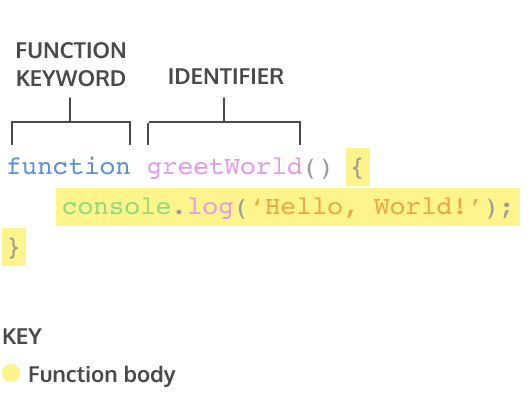
\includegraphics[scale = 0.8]{4_1}
\centering
\end{figure}
\vspace{-4mm}
A function declaration consists of: 
\begin{itemize}[leftmargin = *]
\item The \colorbox{lightgray}{function} keyword.
\item The name of the function, or its identifier, followed by parentheses.
\item A function body, or the block of statements required to perform a specific task, enclosed in the function’s curly brackets, \colorbox{lightgray}{\{ \}}.
\end{itemize}
A function declaration is a function that is bound to an identifier, or name. In the next chapter, we will go over how to run the code inside the function body.
We should also be aware of the \textit{hoisting} feature in JavaScript which allows access to function declarations before they’re defined. Take a look at example of hoisting:
\begin{lstlisting}
console.log(greetWorld()); // Output: Hello, World!

function greetWorld() {
  console.log("Hello, World!");
}
\end{lstlisting}
Notice how hoisting allowed \colorbox{lightgray}{greetWorld()} to be called before the \colorbox{lightgray}{greetWorld()} function was defined! Since hoisting is not considered good practice, we simply want you to be aware of this feature.

\newpage
\subsection{Calling a Function}
As we saw in the previous chapter, a function declaration binds a function to an identifier. However, a function declaration does not ask the code inside the function body to run, it just declares the existence of the function. The code inside a function body runs, or \textit{executes}, only when the function is \textit{called}. To call a function in your code, you type the function name followed by parentheses.
\vspace{-2mm}
\begin{figure}[H]
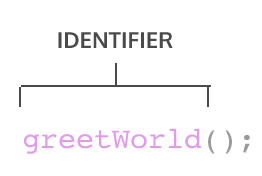
\includegraphics[scale = 0.65]{4_2}
\centering
\end{figure}
\vspace{-3mm}
This \textit{function call} executes the function body, or all of the statements between the curly braces in the function declaration.
\begin{figure}[H]
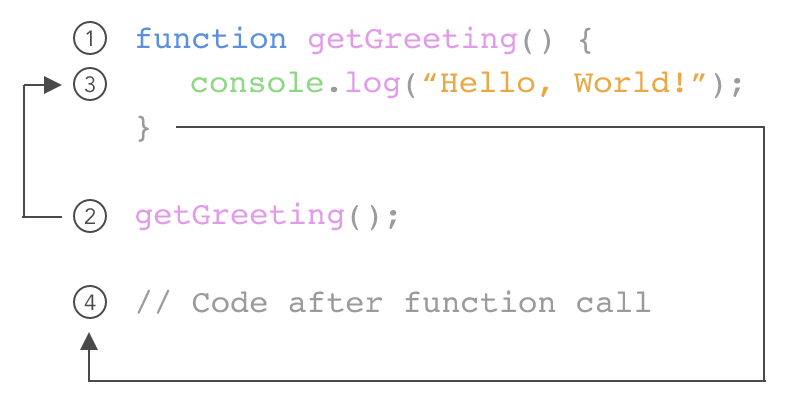
\includegraphics[scale = 0.6]{4_3}
\centering
\end{figure}
We can call the same function as many times as needed.

\subsection{Parameters and Arguments}
So far, the functions we have created execute a task without an input. However, some functions can take inputs and use the inputs to perform a task. When declaring a function, we can specify its \textit{parameters}. Parameters allow functions to accept input(s) and perform a task using the input(s). We use parameters as placeholders for information that will be passed to the function when it is called. \\
\newline
Let’s observe how to specify parameters in our function declaration:
\begin{figure}[H]
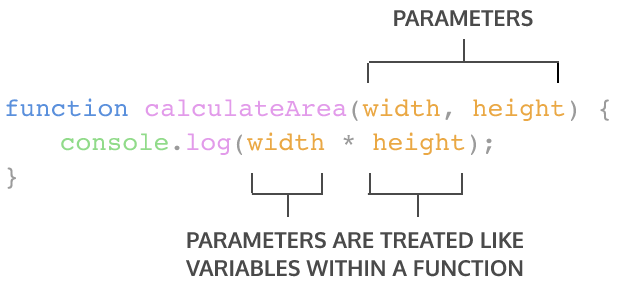
\includegraphics[scale = 0.75]{4_4}
\centering
\end{figure}
In the diagram above, \colorbox{lightgray}{calculateArea()}, computes the area of a rectangle, based on two inputs, \colorbox{lightgray}{width} and \colorbox{lightgray}{height}. The parameters are specified between the parenthesis as \colorbox{lightgray}{width} and \colorbox{lightgray}{height}, and inside the function body, they act just like regular variables. \colorbox{lightgray}{width} and \colorbox{lightgray}{height} act as placeholders for values that will be multiplied together. \\
\newline
When calling a function that has parameters, we specify the values in the parentheses that follow the function name. The values that are passed to the function when it is called are called \textit{arguments}. Arguments can be passed to the function as values or variables.
\begin{figure}[H]
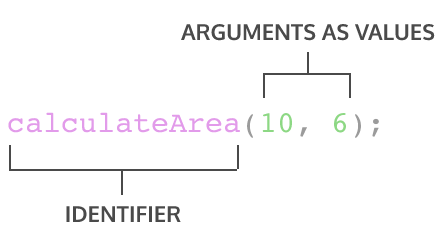
\includegraphics[scale = 0.65]{4_5}
\centering
\end{figure}
In the function call above, the number \colorbox{lightgray}{10} is passed as the \colorbox{lightgray}{width} and \colorbox{lightgray}{6} is passed as \colorbox{lightgray}{height}. Notice that the order in which arguments are passed and assigned follows the order that the parameters are declared.
\begin{figure}[H]
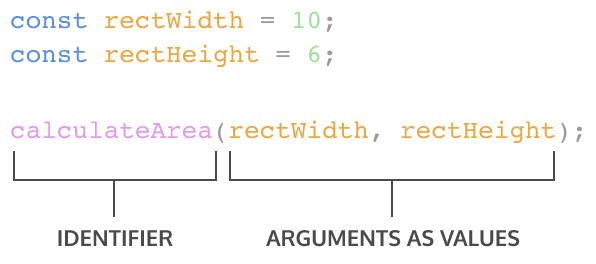
\includegraphics[scale = 0.73]{4_6}
\centering
\end{figure}
The variables \colorbox{lightgray}{rectWidth} and \colorbox{lightgray}{rectHeight} are initialized with the values for the height and width of a rectangle before being used in the function call. \\
\newline
By using parameters, \colorbox{lightgray}{calculateArea()} can be reused to compute the area of any rectangle! Functions are a powerful tool in computer programming so let’s practice creating and calling functions with parameters.

\subsection{Default Parameters}
One of the features added in ES6 is the ability to use \textit{default parameters}. Default parameters allow parameters to have a predetermined value in case there is no argument passed into the function or if the argument is \colorbox{lightgray}{undefined} when called. \\
\newline
Take a look at the code snippet below that uses a default parameter:
\begin{lstlisting}
function greeting (name = "stranger") {
  console.log((*@\texttt{\textasciigrave}@*)Hello, ${name}!(*@\texttt{\textasciigrave}@*))
}

greeting("Nick") // Output: Hello, Nick!
greeting() // Output: Hello, stranger!
\end{lstlisting}
\begin{itemize}[leftmargin = *]
\item In the example above, we used the \colorbox{lightgray}{=} operator to assign the parameter \colorbox{lightgray}{name} a default value of \colorbox{lightgray}{`stranger'}. This is useful to have in case we ever want to include a non-personalized default greeting!
\item When the code calls \colorbox{lightgray}{greeting(`Nick')} the value of the argument is passed in and, \colorbox{lightgray}{`Nick'}, will override the default parameter of \colorbox{lightgray}{`stranger'} to log \colorbox{lightgray}{`Hello, Nick!'} to the console.
\item When there is not an argument passed into \colorbox{lightgray}{greeting()}, the default value of \colorbox{lightgray}{`stranger'} is used, and \colorbox{lightgray}{`Hello, stranger!'} is logged to the console.
\end{itemize}
By using a default parameter, we account for situations when an argument isn’t passed into a function that is expecting an argument.

\subsection{Return}
When a function is called, the computer will run through the function’s code and evaluate the result of calling the function. By default that resulting value is \colorbox{lightgray}{undefined}. 
\begin{lstlisting}
function rectangleArea(width, height) {
  let area = width * height;
}
console.log(rectangleArea(5, 7)) // Prints undefined
\end{lstlisting}
In the code example, we defined our function to calculate the \colorbox{lightgray}{area} of a \colorbox{lightgray}{width} and \colorbox{lightgray}{height} parameter. Then \colorbox{lightgray}{rectangleArea()} is invoked with the arguments \colorbox{lightgray}{5} and \colorbox{lightgray}{7}. But when we went to print the results we got \colorbox{lightgray}{undefined}. The computer did calculate the area as \colorbox{lightgray}{35}, but we did not capture it. But we can capture with the keyword \colorbox{lightgray}{return}. 
\begin{figure}[H]
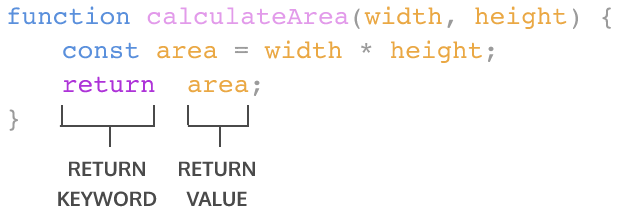
\includegraphics[scale = 0.73]{4_7}
\centering
\end{figure}
To pass back information from the function call, we use a return statement. To create a return statement, we use the \colorbox{lightgray}{return} keyword followed by the value that we wish to return. Like we saw above, if the value is omitted, \colorbox{lightgray}{undefined} is returned instead. \\
\newline
When a \colorbox{lightgray}{return} statement is used in a function body, the execution of the function is stopped and the code that follows it will not be executed. Look at the example below:
\begin{lstlisting}
function rectangleArea(width, height) {
  if (width < 0 || height < 0) {
    return "You need positive integers to calculate area!";
  }
  return width * height;
}
\end{lstlisting}
If an argument for \colorbox{lightgray}{width} or \colorbox{lightgray}{height} is less than \colorbox{lightgray}{0}, then \colorbox{lightgray}{rectangleArea()} will return the string \\ 
\colorbox{lightgray}{`You need positive integers to calculate area!'}. The second return statement \colorbox{lightgray}{width * height} will not run.

The \colorbox{lightgray}{return} keyword is powerful because it allows functions to produce an output. We can then save the output to a variable for later use.

\subsection{Helper Functions}
We can also use the return value of a function inside another function. These functions being called within another function are often referred to as \textit{helper functions}. Since each function is carrying out a specific task, it makes our code easier to read and debug if necessary. \\
\newline
If we wanted to define a function that converts the temperature from Celsius to Fahrenheit, we could write two functions like:
\begin{lstlisting}
function multiplyByNineFifths(number) {
  return number * (9/5);
};

function getFahrenheit(celsius) {
  return multiplyByNineFifths(celsius) + 32;
};

getFahrenheit(15); // Returns 59
\end{lstlisting}

In the example above: 
\begin{itemize}[leftmargin = *]
\item \colorbox{lightgray}{getFahrenheit()} is called and \colorbox{lightgray}{15} is passed as an argument.
\item The code block inside of \colorbox{lightgray}{getFahrenheit()} calls \colorbox{lightgray}{multiplyByNineFifths()} and passes \colorbox{lightgray}{15} as an argument.
\item \colorbox{lightgray}{multiplyByNineFifths()} takes the argument of \colorbox{lightgray}{15} for the \colorbox{lightgray}{number} parameter.
\item The code block inside of \colorbox{lightgray}{multiplyByNineFifths()} function multiplies \colorbox{lightgray}{15} by \colorbox{lightgray}{(9/5)}, which evaluates to \colorbox{lightgray}{27}.
\item \colorbox{lightgray}{27} is returned back to the function call in \colorbox{lightgray}{getFahrenheit()}.
\item \colorbox{lightgray}{getFahrenheit()} continues to execute. It adds \colorbox{lightgray}{32} to \colorbox{lightgray}{27}, which evaluates to \colorbox{lightgray}{59}.
\item Finally, \colorbox{lightgray}{59} is returned back to the function call \colorbox{lightgray}{getFahrenheit(15)}.
\end{itemize}
We can use functions to section off small bits of logic or tasks, then use them when we need to. Writing helper functions can help take large and difficult tasks and break them into smaller and more manageable tasks.
\newpage
\subsection{Function Expressions}
Another way to define a function is to use a \textit{function expression}. To define a function inside an expression, we can use the \colorbox{lightgray}{function} keyword. In a function expression, the function name is usually omitted. A function with no name is called an \textit{anonymous function}. A function expression is often stored in a variable in order to refer to it. Consider the following function expression:
\begin{figure}[H]
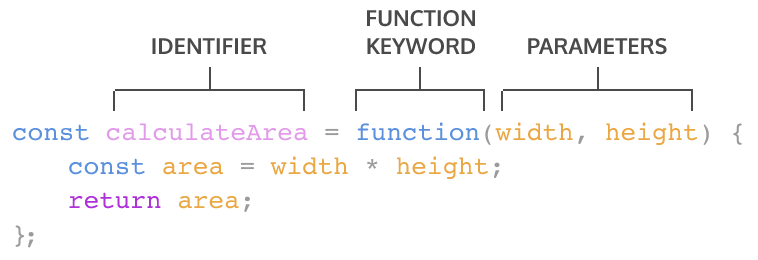
\includegraphics[scale = 0.73]{4_8}
\centering
\end{figure}
To declare a function expression:
\begin{enumerate}[leftmargin = *]
\item Declare a variable to make the variable’s name be the name, or identifier, of your function. Since the release of ES6, it is common practice to use \colorbox{lightgray}{const} as the keyword to declare the variable.
\item Assign as that variable’s value an anonymous function created by using the \colorbox{lightgray}{function} keyword followed by a set of parentheses with possible parameters. Then a set of curly braces that contain the function body.
\end{enumerate}
To invoke a function expression, write the name of the variable in which the function is stored followed by parentheses enclosing any arguments being passed into the function.
\begin{lstlisting}
variableName(argument1, argument2)
\end{lstlisting}
Unlike function declarations, function expressions are not hoisted so they cannot be called before they are defined.

\subsection{Arrow Functions}
ES6 introduced \textit{arrow function syntax}, a shorter way to write functions by using the special “fat arrow” \colorbox{lightgray}{$($$)$ $=$$>$} notation. \\
\newline
Arrow functions remove the need to type out the keyword \colorbox{lightgray}{function} every time you need to create a function. Instead, you first include the parameters inside the \colorbox{lightgray}{( )} and then add an arrow \colorbox{lightgray}{$=$$>$} that points to the function body surrounded in \colorbox{lightgray}{\{ \}} like this:
\begin{lstlisting}
const rectangleArea = (width, height) => {
  let area = width * height;
  return area;
};
\end{lstlisting}
It is important to be familiar with the multiple ways of writing functions because you will come across each of these when reading other JavaScript code.

\subsection{Concise Body Arrow Functions}
JavaScript also provides several ways to refactor arrow function syntax. The most condensed form of the function is known as \textit{concise body}. We will explore a few of these techniques below:
\begin{enumerate}[leftmargin = *]
\item Functions that take only a single parameter do not need that parameter to be enclosed in parentheses. However, if a function takes zero or multiple parameters, parentheses are required.
\begin{figure}[H]
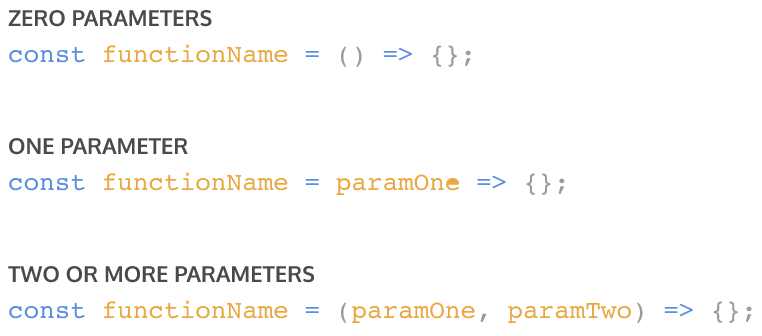
\includegraphics[scale = 0.73]{4_9}
\centering
\end{figure}
\item A function body composed of a single-line block does not need curly braces. Without the curly braces, whatever that line evaluates will be automatically returned. The contents of the block should immediately follow the arrow \colorbox{lightgray}{$=$$>$} and the \colorbox{lightgray}{return} keyword can be removed. This is referred to as \textit{implicit return}.
\end{enumerate}
\begin{figure}[H]
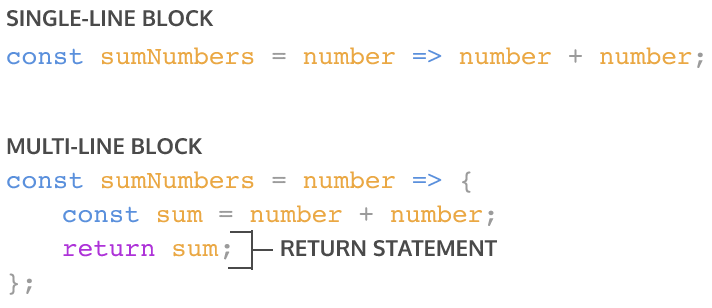
\includegraphics[scale = 0.73]{4_10}
\centering
\end{figure}
So if we have a function: 
\begin{lstlisting}
const squareNum = (num) => {
  return num * num;
};
\end{lstlisting}
We can refactor the function to:
\begin{lstlisting}
const squareNum = num => num * num;
\end{lstlisting}
Notice the following changes:
\begin{itemize}[leftmargin = *]
\item The parentheses around \colorbox{lightgray}{num} have been removed, since it has a single parameter.
\item The curly braces \colorbox{lightgray}{\{ \}} have been removed since the function consists of a single-line block.
\item The \colorbox{lightgray}{return} keyword has been removed since the function consists of a single-line block.
\end{itemize}

\subsection{Review Functions}
In this we covered some important concepts about functions:
\begin{itemize}[leftmargin = *]
\item A \textit{function} is a reusable block of code that groups together a sequence of statements to perform a specific task.
\item A \textit{function declaration}:
\vspace{-4mm}
\begin{figure}[H]
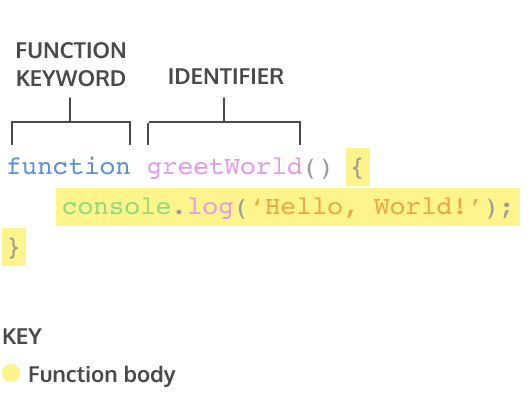
\includegraphics[scale = 0.73]{4_1}
\centering
\end{figure}
\item A parameter is a named variable inside a function’s block which will be assigned the value of the argument passed in when the function is invoked: 
\begin{figure}[H]
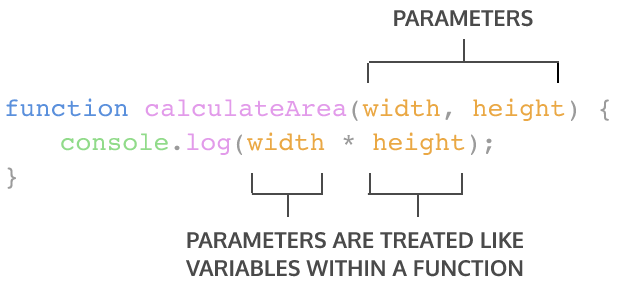
\includegraphics[scale = 0.75]{4_4}
\centering
\end{figure}
\item To \textit{call} a function in your code:
\vspace{-2mm}
\begin{figure}[H]
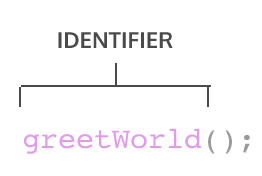
\includegraphics[scale = 0.65]{4_2}
\centering
\end{figure}
\item ES6 introduces new ways of handling arbitrary parameters through \textit{default parameters} which allow us to assign a default value to a parameter in case no argument is passed into the function.
\item To return a value from a function, we use a \textit{return statement}.
\item To define a function using \textit{function} expressions:
\begin{figure}[H]
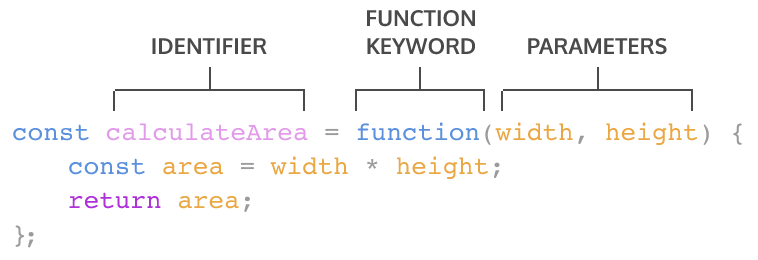
\includegraphics[scale = 0.73]{4_8}
\centering
\end{figure}
\item To define a function using \textit{arrow function notation}:
\begin{figure}[H]
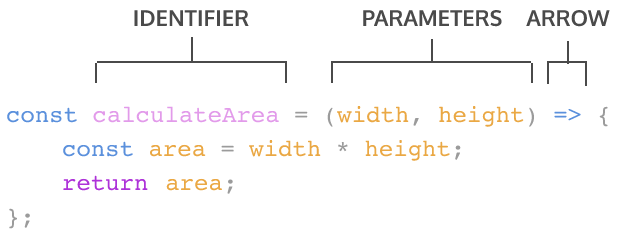
\includegraphics[scale = 0.8]{4_11}
\centering
\end{figure}
\item Function definition can be made concise using concise arrow notation:
\begin{figure}[H]
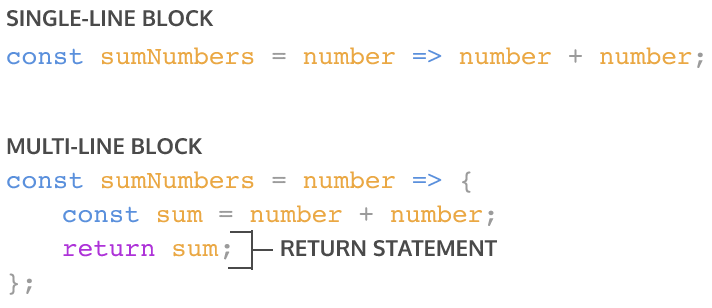
\includegraphics[scale = 0.73]{4_10}
\centering
\end{figure}
\end{itemize}
It is good to be aware of the differences between function expressions, arrow functions, and function declarations. As you program more in JavaScript, you will see a wide variety of how these function types are used. 

\newpage
\section{Scope}
\subsection{Scope}
An important idea in programming is \textit{scope}. Scope defines where variables can be accessed or referenced. While some variables can be accessed from anywhere within a program, other variables may only be available in a specific context. \\
\newline
You can think of scope like the view of the night sky from your window. Everyone who lives on the planet Earth is in the global scope of the stars. The stars are accessible \textit{globally}. Meanwhile, if you live in a city, you may see the city skyline or the river. The skyline and river are only accessible \textit{locally} in your city, but you can still see the stars that are available globally. \\
\newline
Over the next few chapters, we will explore how scope relates to variables and learn best practices for variable declaration.

\subsection{Blocks and Scope}
Before we talk more about scope, we first need to talk about \textit{blocks}. We have seen blocks used before in functions and \colorbox{lightgray}{if} statements. A block is the code found inside a set of curly braces \colorbox{lightgray}{\{\}}. Blocks help us group one or more statements together and serve as an important structural marker for our code. \\
\newline
A block of code could be a function, like this: 
\begin{lstlisting}
const logSkyColor = () => {
  let color = "blue"; 
  console.log(color); // blue 
};
\end{lstlisting}
Notice that the function body is actually a block of code. Observe the block in an \colorbox{lightgray}{if} statement:
\begin{lstlisting}
if (dusk) {
  let color = "pink";
  console.log(color); // pink
};
\end{lstlisting}
In the next few chapters, we will see how blocks define the scope of variables.

\subsection{Global Scope}
Scope is the context in which our variables are declared. We think about scope in relation to blocks because variables can exist either outside of or within these blocks. \\
\newline
In \textit{global scope}, variables are declared outside of blocks. These variables are called \textit{global variables}. Because global variables are not bound inside a block, they can be accessed by any code in the program, including code in blocks. \\
\newpage
Let us take a look at an example of global scope:
\begin{lstlisting}
const color = "blue"

const returnSkyColor = () => {
  return color; // blue 
};

console.log(returnSkyColor()); // blue
\end{lstlisting}
\begin{itemize}[leftmargin = *]
\item Even though the \colorbox{lightgray}{color} variable is defined outside of the block, it can be accessed in the function block, giving it global scope.
\item In turn, \colorbox{lightgray}{color} can be accessed within the \colorbox{lightgray}{returnSkyColor} function block.
\end{itemize}

\subsection{Block Scope}
The next context we will cover is \textit{block scope}. When a variable is defined inside a block, it is only accessible to the code within the curly braces \colorbox{lightgray}{\{\}}. We say that variable has \textit{block scope} because it is \textit{only} accessible to the lines of code within that block. \\
\newline
Variables that are declared with block scope are known as \textit{local variables} because they are only available to the code that is part of the same block. \\
\newline
Block scope works like this:
\begin{lstlisting}
const logSkyColor = () => {
  let color = "blue"; 
  console.log(color); // blue 
};

logSkyColor(); // blue 
console.log(color); // ReferenceError
\end{lstlisting}
We will notice:
\begin{itemize}[leftmargin = *]
\item We define a function  \colorbox{lightgray}{logSkyColor()}.
\item Within the function, the  \colorbox{lightgray}{color} variable is only available within the curly braces of the function.
\item If we try to log the same variable outside the function, throws a  \colorbox{lightgray}{ReferenceError}.
\end{itemize}

\subsection{Scope Pollution}
It may seem like a great idea to always make your variables accessible, but having too many global variables can cause problems in a program. \\
\newline
When you declare global variables, they go to the \textit{global namespace}. The global namespace allows the variables to be accessible from anywhere in the program. These variables remain there until the program finishes which means our global namespace can fill up really quickly. \\
\newline
\textit{Scope pollution} is when we have too many global variables that exist in the global namespace, or when we reuse variables across different scopes. Scope pollution makes it difficult to keep track of our different variables and sets us up for potential accidents. For example, globally scoped variables can collide with other variables that are more locally scoped, causing unexpected behavior in our code. \\
\newline
Let us look at an example of scope pollution in practice so we know how to avoid it:
\begin{lstlisting}
let num = 50;

const logNum = () => {
  num = 100; // Take note of this line of code
  console.log(num);
};

logNum(); // Prints 100
console.log(num); // Prints 100
\end{lstlisting}
We will notice:
\begin{itemize}[leftmargin = *]
\item We have a variable \colorbox{lightgray}{num}.
\item Inside the function body of \colorbox{lightgray}{logNum()}, we want to declare a new variable but forgot to use the \colorbox{lightgray}{let} keyword.
\item When we call \colorbox{lightgray}{logNum()}, \colorbox{lightgray}{num} gets reassigned to \colorbox{lightgray}{100}.
\item The reassignment inside \colorbox{lightgray}{logNum()} affects the global variable \colorbox{lightgray}{num}.
\item Even though the reassignment is allowed and we will not get an error, if we decided to use \colorbox{lightgray}{num} later, we’ll unknowingly use the new value of \colorbox{lightgray}{num}.
\end{itemize}
While it is important to know what global scope is, it is best practice to not define variables in the global scope.

\subsection{Practice Good Scoping}
Given the challenges with global variables and scope pollution, we should follow best practices for scoping our variables as tightly as possible using block scope. \\
\newline
Tightly scoping your variables will greatly improve your code in several ways:
\begin{itemize}[leftmargin = *]
\item It will make your code more legible since the blocks will organize your code into discrete sections. 
\item It makes your code more understandable since it clarifies which variables are associated with different parts of the program rather than having to keep track of them line after line! 
\item It is easier to maintain your code, since your code will be modular.
\item It will save memory in your code because it will cease to exist after the block finishes running.
\end{itemize}
Here is another example of how to use block scope, as defined within an \colorbox{lightgray}{if} block:
\begin{lstlisting}
const logSkyColor = () => {
  const dusk = true;
  let color = "blue"; 
  if (dusk) {
    let color = "pink";
    console.log(color); // pink
  }
  console.log(color); // blue 
};

console.log(color); // ReferenceError
\end{lstlisting}
Here, we will notice:
\begin{itemize}[leftmargin = *]
\item We create a variable \colorbox{lightgray}{dusk} inside the \colorbox{lightgray}{logSkyColor()} function.
\item After the \colorbox{lightgray}{if} statement, we define a new code block with the \colorbox{lightgray}{\{\}} braces. Here we assign a new value to the variable \colorbox{lightgray}{color} if the \colorbox{lightgray}{if} statement is truthy.
\item Within the \colorbox{lightgray}{if} block, the \colorbox{lightgray}{color} variable holds the value \colorbox{lightgray}{`pink'}, though outside the \colorbox{lightgray}{if} block, in the function body, the \colorbox{lightgray}{color} variable holds the value \colorbox{lightgray}{`blue'}.
\item While we use block scope, we still pollute our namespace by reusing the same variable name twice. A better practice would be to rename the variable inside the block.
\end{itemize}
Block scope is a powerful tool in JavaScript, since it allows us to define variables with precision, and not pollute the global namespace. If a variable does not need to exist outside a block, then it should not!

\subsection{Review: Scope}
In this chapter, you learned about scope and how it impacts the accessibility of different variables. \\
Let us review the following terms:
\begin{itemize}[leftmargin = *]
\item \textbf{Scope} is the idea in programming that some variables are accessible/inaccessible from other parts of the program.
\item \textbf{Blocks} are statements that exist within curly braces \colorbox{lightgray}{\{\}}.
\item \textbf{Global scope} refers to the context within which variables are accessible to every part of the program.
\item \textbf{Global variables} are variables that exist within global scope.
\item \textbf{Block scope} refers to the context within which variables that are accessible only within the block they are defined.
\item \textbf{Local variables} are variables that exist within block scope.
\item \textbf{Global namespace} is the space in our code that contains globally scoped information.
\item \textbf{Scope pollution} is when too many variables exist in a namespace or variable names are reused.
\end{itemize}

\newpage
\section{Arrays}
\subsection{Arrays}
Organizing and storing data is a foundational concept of programming. One way we organize data in real life is by making lists. Let us make one here:
\begin{lstlisting}
(*@New Year's Resolutions:@*)
(*@1. Keep a journal @*)
(*@2. Take a falconry class@*)
(*@3. Learn to juggle@*)
\end{lstlisting}
Let us now write this list in JavaScript, as an array:
\begin{lstlisting}
let newYearsResolutions = ["Keep a journal", "Take a falconry class", "Learn to juggle"];
\end{lstlisting}
Arrays are JavaScript’s way of making lists. Arrays can store any data types (including strings, numbers, and booleans). Like lists, arrays are ordered, meaning each item has a numbered position.
Here is an array of the concepts we’ll cover:
\begin{lstlisting}
let concepts = ["creating arrays", "array structures", "array manipulation"];
\end{lstlisting}

\subsection{Create an Array}
One way we can create an array is to use an \textit{array literal}. An array literal creates an array by wrapping items in square brackets \colorbox{lightgray}{$[$ $]$}. Remember from the previous exercise, arrays can store any data type — we can have an array that holds all the same data types or an array that holds different data types.
\begin{figure}[H]
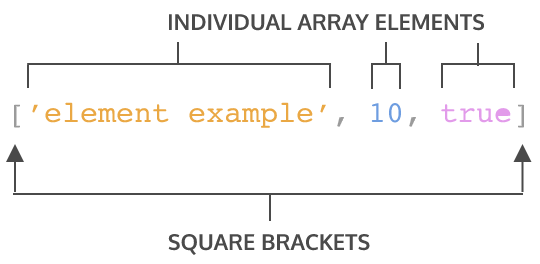
\includegraphics[scale = 0.65]{6_1}
\centering
\end{figure}
Let us take a closer look at the syntax in the array example:
\begin{itemize}[leftmargin = *]
\item The array is represented by the square brackets \colorbox{lightgray}{$[$ $]$} and the content inside.
\item Each content item inside an array is called an \textit{element}.
\item There are three different elements inside the array.
Each element inside the array is a different data type.
\end{itemize}
We can also save an array to a variable. You may have noticed we did this in the previous chapter:
\begin{lstlisting}
let newYearsResolutions = ['Keep a journal', 'Take a falconry class', 'Learn to juggle'];
\end{lstlisting}
\subsection{Accessing Elements}
Each element in an array has a numbered position known as its \textit{index}. We can access individual items using their index, which is similar to referencing an item in a list based on the item’s position. \\
\newline
Arrays in JavaScript are \textit{zero-indexed}, meaning the positions start counting from \colorbox{lightgray}{0} rather than \colorbox{lightgray}{1}. Therefore, the first item in an array will be at position \colorbox{lightgray}{0}. Let us see how we could access an element in an array:
\begin{figure}[H]
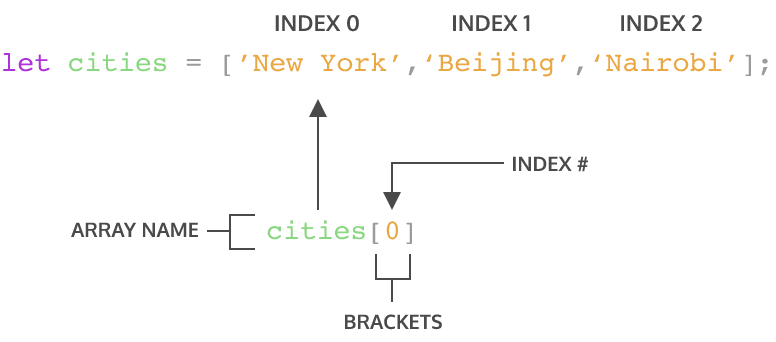
\includegraphics[scale = 0.65]{6_2}
\centering
\end{figure}
In the code snippet above:
\begin{itemize}[leftmargin = *]
\item \colorbox{lightgray}{cities} is an array that has three elements.
\item We are using bracket notation, \colorbox{lightgray}{$[$ $]$} with the index after the name of the array to access the element.
\item \colorbox{lightgray}{cities[0]} will access the element at index \colorbox{lightgray}{0} in the array \colorbox{lightgray}{cities}. You can think of \colorbox{lightgray}{cities[0]} as accessing the space in memory that holds the string \colorbox{lightgray}{`New York'}.
\end{itemize}
You can also access individual characters in a string using bracket notation and the index. For instance, you can write:
\begin{lstlisting}
const hello = "Hello World";
console.log(hello[6]); // Output: W
\end{lstlisting}
The console will display \colorbox{lightgray}{W} since it is the character that is at index \colorbox{lightgray}{6}.\\
\newline
If you try to access an index that is beyond the last element, console will return \colorbox{lightgray}{undefined}. 

\subsection{Update Elements} 
In the previous exercise, you learned how to access elements inside an array or a string by using an index. Once you have access to an element in an array, you can update its value. 
\begin{lstlisting}
let seasons = ["Winter", "Spring", "Summer", "Fall"];

seasons[3] = "Autumn";
console.log(seasons); 
//Output: ["Winter", "Spring", "Summer", "Autumn"]
\end{lstlisting}
In the example above, the \colorbox{lightgray}{seasons} array contained the names of the four seasons. However, we decided that we preferred to say \colorbox{lightgray}{`Autumn'} instead of \colorbox{lightgray}{`Fall'}. The line, \colorbox{lightgray}{seasons[3] = `Autumn';} tells our program to change the item at index 3 of the seasons array to be \colorbox{lightgray}{`Autumn'} instead of what is already there.

\subsection{Arrays with let and const}
You may recall that you can declare variables with both the \colorbox{lightgray}{let} and \colorbox{lightgray}{const} keywords. Variables declared with \colorbox{lightgray}{let} can be reassigned. \\
\newline
Variables declared with the \colorbox{lightgray}{const} keyword cannot be reassigned. However, elements in an array declared with \colorbox{lightgray}{const} remain mutable. Meaning that we can change the contents of a \colorbox{lightgray}{const} array, but cannot reassign a new array or a different value. \\
\newline
The instructions below will illustrate this concept more clearly. Pay close attention to the similarities and differences between the \colorbox{lightgray}{condiments} array and the \colorbox{lightgray}{utensils} array as you complete the steps.
\begin{lstlisting}
let condiments = ["Ketchup", "Mustard", "Soy Sauce", "Sriracha"];
const utensils = ["Fork", "Knife", "Chopsticks", "Spork"];

condiments[0] = "Mayo";
console.log(condiments); 
// Output: [ "Mayo", "Mustard", "Soy Sauce", "Sriracha" ]

condiments = ["Mayo"]; 
console.log(condiments); 
// Output: [ "Mayo" ]

utensils[3] = "Spoon";
console.log(utensils); 
// Output: [ "Fork", "Knife", "Chopsticks", "Spoon" ]

utensils = ["Spoon"]; 
// TypeError: Assignment to constant variable.
\end{lstlisting}

\subsection{The .length property}
One of an array’s built-in properties is \colorbox{lightgray}{length} and it returns the number of items in the array. We access the \colorbox{lightgray}{.length} property just like we do with strings. Check the example below: 
\begin{lstlisting}
const newYearsResolutions = ["Keep a journal", "Take a falconry class"];

console.log(newYearsResolutions.length); // Output: 2
\end{lstlisting}
In the example above, we log \colorbox{lightgray}{newYearsResolutions.length} to the console using the following steps:
\begin{itemize}[leftmargin = *]
\item We use \textit{dot notation}, chaining a period with the property name to the array, to access the \colorbox{lightgray}{length} property of the \colorbox{lightgray}{newYearsResolutions} array.
\item Then we log the \colorbox{lightgray}{length} of \colorbox{lightgray}{newYearsResolution} to the console.
\item Since \colorbox{lightgray}{newYearsResolution} has two elements, so \colorbox{lightgray}{2} would be logged to the console.
\end{itemize}
When we want to know how many elements are in an array, we can access the \colorbox{lightgray}{.length} property.

\subsection{The .push() Method}
Let us learn about some built-in JavaScript methods that make working with arrays easier. These methods are specifically called on arrays to make common tasks, like adding and removing elements, more straightforward. \\
\newline
One method, \colorbox{lightgray}{.push()} allows us to add items to the end of an array. Here is an example of how this is used:
\begin{lstlisting}
const itemTracker = ["item 0", "item 1", "item 2"];

itemTracker.push("item 3", "item 4");

console.log(itemTracker); 
// Output: ["item 0", "item 1", "item 2", "item 3", "item 4"];
\end{lstlisting}
So, how does \colorbox{lightgray}{.push()} work?
\begin{itemize}[leftmargin = *]
\item We access the \colorbox{lightgray}{push} method by using dot notation, connecting \colorbox{lightgray}{push} to \colorbox{lightgray}{itemTracker} with a period.
\item Then we call it like a function. That is because \colorbox{lightgray}{.push()} is a function and one that JavaScript allows us to use right on an array.
\item \colorbox{lightgray}{.push()} can take a single argument or multiple arguments separated by commas. In this case, we’re adding two elements: \colorbox{lightgray}{`item 3'} and \colorbox{lightgray}{`item 4'} to \colorbox{lightgray}{itemTracker}.
\item Notice that \colorbox{lightgray}{.push()} changes, or \textit{mutates}, itemTracker. You might also see \colorbox{lightgray}{.push()} referred to as a \textit{destructive} array method since it changes the initial array.
\end{itemize}
If you are looking for a method that will mutate an array by adding elements to it, then \colorbox{lightgray}{.push()} is the method for you. 

\subsection{The .pop() Method}
Another array method, \colorbox{lightgray}{.pop()}, removes the last item of an array.
\begin{lstlisting}
const newItemTracker = ["item 0", "item 1", "item 2"];

const removed = newItemTracker.pop();

console.log(newItemTracker); // Output: [ "item 0", "item 1" ]
console.log(removed); // Output: item 2
\end{lstlisting}
\begin{itemize}[leftmargin = *]
\item In the example above, calling \colorbox{lightgray}{.pop()} on the \colorbox{lightgray}{newItemTracker} array removed \colorbox{lightgray}{item 2} from the end.
\item \colorbox{lightgray}{.pop()} does not take any arguments, it simply removes the last element of \colorbox{lightgray}{newItemTracker}.
\item \colorbox{lightgray}{.pop()} returns the value of the last element. In the example, we store the returned value in a variable \colorbox{lightgray}{removed} to be used for later.
\item \colorbox{lightgray}{.pop()} is a method that mutates the initial array.

\end{itemize}
When you need to mutate an array by removing the last element, use \colorbox{lightgray}{.pop()}.

\subsection{More Array Methods}
There are many more array methods than just \colorbox{lightgray}{.push()} and \colorbox{lightgray}{.pop()}. You can read about all of the array methods that exist on the \href{https://developer.mozilla.org/en-US/docs/Web/JavaScript/Reference/Global_Objects/Array}{Mozilla Developer Network (MDN) array documentation}. \\
\newline
\colorbox{lightgray}{.pop()} and \colorbox{lightgray}{.push()} mutate the array on which they are called. However, there are times that we do not want to mutate the original array and we can use non-mutating array methods. \\
\newline
Some arrays methods that are available to JavaScript developers include: \colorbox{lightgray}{.join()}, \colorbox{lightgray}{.slice()}, \colorbox{lightgray}{.splice()}, \colorbox{lightgray}{.shift()}, \colorbox{lightgray}{.unshift()}, and \colorbox{lightgray}{.concat()} amongst many others. Using these built-in methods make it easier to do some common tasks when working with arrays. \\
\newline
Below, we will explore \colorbox{lightgray}{.shift()}, \colorbox{lightgray}{.unshift()}, and \colorbox{lightgray}{.slice()}. 

\subsubsection{The .shift() Method}
The \colorbox{lightgray}{.shift()} method removes the first element from an array and returns that removed element. This method changes the length of the array. The original array is modified. 
\begin{lstlisting}
const array1 = [1, 2, 3];
const firstElement = array1.shift();
console.log(array1); // Output: Array [2, 3]

console.log(firstElement); // Output: 1
\end{lstlisting}

\subsubsection{The .unshift() Method}
The \colorbox{lightgray}{.unshift()} method adds one or more elements to the beginning of an array and returns the new length of the array. The original array is modified. 
\begin{lstlisting}
const array1 = [1, 2, 3];
console.log(array1.unshift(4, 5)); // Output: 5

console.log(array1); // Output: Array [4, 5, 1, 2, 3]
\end{lstlisting}

\subsubsection{The .slice() Method}
The \colorbox{lightgray}{.slice()} method returns a shallow copy of a portion of an array into a new array object selected from start to end (end not included) where start and end represent the index of items in that array. The original array will not be modified.
\begin{lstlisting}
const animals = ["ant", "bison", "camel", "duck", "elephant"];
console.log(animals.slice(2)); // Output: Array ["camel", "duck", "elephant"]

console.log(animals.slice(2, 4)); // Output: Array ["camel", "duck"]

console.log(animals.slice(1, 5)); 
// Output: Array ["bison", "camel", "duck", "elephant"]
\end{lstlisting}

\subsection{Arrays and Functions}
Throughout the lesson we went over arrays being mutable, or changeable. What happens if we try to change an array inside a function? Does the array keep the change after the function call or is it scoped to inside the function? \\
\newline
Take a look at the following example where we call \colorbox{lightgray}{.push()} on an array inside a function. Recall, the \colorbox{lightgray}{.push()} method mutates, or changes, an array:
\begin{lstlisting}
const flowers = ["peony", "daffodil", "marigold"];

function addFlower(arr) {
  arr.push("lily");
}

addFlower(flowers);
console.log(flowers); // Output: ["peony", "daffodil", "marigold", "lily"]
\end{lstlisting}
Let’s go over what happened in the example:
\begin{itemize}[leftmargin = *]
\item The \colorbox{lightgray}{flowers} array that has 3 elements.
\item The function \colorbox{lightgray}{addFlower()} has a parameter of \colorbox{lightgray}{arr} uses \colorbox{lightgray}{.push()} to add a \colorbox{lightgray}{`lily'} element into \colorbox{lightgray}{arr}.
\item We call \colorbox{lightgray}{addFlower()} with an argument of \colorbox{lightgray}{flowers} which will execute the code inside \colorbox{lightgray}{addFlower}.
\item We check the value of \colorbox{lightgray}{flowers} and it now includes the \colorbox{lightgray}{`lily'} element! The array was mutated!
\end{itemize}
So when you pass an array into a function, if the array is mutated inside the function, that change will be maintained outside the function as well. You might also see this concept explained as \textit{pass-by-reference} since what we are actually passing the function is a reference to where the variable memory is stored and changing the memory.

\subsection{Nested Arrays}
Earlier we mentioned that arrays can store other arrays. When an array contains another array it is known as a \textit{nested array}. Examine the example below:
\begin{lstlisting}
const nestedArr = [[1], [2, 3]];
\end{lstlisting}
To access the nested arrays we can use bracket notation with the index value, just like we did to access any other element:
\begin{lstlisting}
const nestedArr = [[1], [2, 3]];

console.log(nestedArr[1]); // Output: [2, 3]
\end{lstlisting}
Notice that \colorbox{lightgray}{nestedArr[1]} will grab the element in index 1 which is the array \colorbox{lightgray}{[2, 3]}. Then, if we wanted to access the elements within the nested array we can \textit{chain}, or add on, more bracket notation with index values. 
\begin{lstlisting}
const nestedArr = [[1], [2, 3]];

console.log(nestedArr[1]); // Output: [2, 3]
console.log(nestedArr[1][0]); // Output: 2
\end{lstlisting}
In the second \colorbox{lightgray}{console.log()} statement, we have two bracket notations chained to \colorbox{lightgray}{nestedArr}. We know that \colorbox{lightgray}{nestedArr[1]} is the array \colorbox{lightgray}{[2, 3]}. Then to grab the first element from that array, we use \colorbox{lightgray}{nestedArr[1][0]} and we get the value of \colorbox{lightgray}{2}.

\subsection{Review Arrays}
In this chapter, we learned these concepts regarding arrays:
\begin{itemize}[leftmargin = *]
\item Arrays are lists that store data in JavaScript.
\item Arrays are created with brackets \colorbox{lightgray}{$[$ $]$}.
\item Each item inside of an array is at a numbered position, or index, starting at \colorbox{lightgray}{0}.
\item We can access one item in an array using its index, with syntax like: \colorbox{lightgray}{myArray[0]}.
\item We can also change an item in an array using its index, with syntax like \colorbox{lightgray}{myArray[0] = `new string'};
\item Arrays have a \colorbox{lightgray}{length} property, which allows you to see how many items are in an array.
\item Arrays have their own methods, including \colorbox{lightgray}{.push()} and \colorbox{lightgray}{.pop()}, which add and remove items from an array, respectively.
\item Arrays have many methods that perform different tasks, such as \colorbox{lightgray}{.slice()} and \colorbox{lightgray}{.shift()}, you can find documentation at the Mozilla Developer Network website.
\item Some built-in methods are mutating, meaning the method will change the array, while others are not mutating. You can always check the documentation.
\item Variables that contain arrays can be declared with \colorbox{lightgray}{let} or \colorbox{lightgray}{const}. Even when declared with \colorbox{lightgray}{const}, arrays are still mutable. However, a variable declared with \colorbox{lightgray}{const} cannot be reassigned.
\item Arrays mutated inside of a function will keep that change even outside the function.
\item Arrays can be nested inside other arrays.
\item To access elements in nested arrays chain indices using bracket notation.
\end{itemize}
Learning how to work with and manipulate arrays will help you work with chunks of data. 

\newpage
\section{Loops}
\subsection{Loops}
A \textit{loop} is a programming tool that repeats a set of instructions until a specified condition, called a \textit{stopping condition} is reached. As a programmer, you will find that you rely on loops all the time! You’ll hear the generic term iterate when referring to loops; \textit{iterate} simply means “to repeat”. \\
\newline
When we need to reuse a task in our code, we often bundle that action in a function. Similarly, when we see that a process has to repeat multiple times in a row, we write a loop. Loops allow us to create efficient code that automates processes to make scalable, manageable programs. \\
\newline
Loops iterate or repeat an action until a specific condition is met. When the condition is met, the loop stops and the computer moves on to the next part of the program.

\subsection{The For Loop}
Instead of writing out the same code over and over, loops allow us to tell computers to repeat a given block of code on its own. One way to give computers these instructions is with a \colorbox{lightgray}{for} loop. \\
\newline
The typical \colorbox{lightgray}{for} loop includes an \textit{iterator variable} that usually appears in all three expressions. The iterator variable is initialized, checked against the stopping condition, and assigned a new value on each loop iteration. Iterator variables can have any name, but it is best practice to use a descriptive variable name. \\
\newline
A \colorbox{lightgray}{for} loop contains three expressions separated by \colorbox{lightgray}{;} inside the parentheses:
\begin{enumerate}[leftmargin = *]
\item an \textit{initialization} starts the loop and can also be used to declare the iterator variable.
\item a \textit{stopping condition} is the condition that the iterator variable is evaluated against— if the condition evaluates to \colorbox{lightgray}{true} the code block will run, and if it evaluates to \colorbox{lightgray}{false} the code will stop.
\item an \textit{iteration statement} is used to update the iterator variable on each loop.
\end{enumerate}
The \colorbox{lightgray}{for} loop syntax looks like this:
\begin{lstlisting}
for (let counter = 0; counter < 4; counter++) {
  console.log(counter);
}
\end{lstlisting}
In this example, the output would be the following:
\begin{lstlisting}
0
1
2
3
\end{lstlisting}
Let us break down the example:
\begin{itemize}[leftmargin = *]
\item The initialization is \colorbox{lightgray}{let counter = 0}, so the loop will start counting at \colorbox{lightgray}{0}.
\item The stopping condition is \colorbox{lightgray}{counter < 4}, meaning the loop will run as long as the iterator variable, \colorbox{lightgray}{counter}, is less than 4.
\item The iteration statement is \colorbox{lightgray}{counter++}. This means after each loop, the value of \colorbox{lightgray}{counter} will increase by 1. For the first iteration \colorbox{lightgray}{counter} will equal \colorbox{lightgray}{0}, for the second iteration \colorbox{lightgray}{counter} will equal 1, and so on.
\item The code block is inside of the curly braces, \colorbox{lightgray}{console.log(counter)}, will execute until the condition evaluates to \colorbox{lightgray}{false}. The condition will be \colorbox{lightgray}{false} when counter is greater than or equal to 4 — the point that the condition becomes false is sometimes called the \textit{stop condition}.
\end{itemize}
This \colorbox{lightgray}{for} loop makes it possible to write 0, 1, 2, and 3 programmatically.

\subsection{Looping in Reverse}

What if we want the \colorbox{lightgray}{for} loop to log \colorbox{lightgray}{3}, \colorbox{lightgray}{2}, \colorbox{lightgray}{1}, and then \colorbox{lightgray}{0}? With simple modifications to the expressions, we can make our loop run backward. \\
\newline
To run a backward \colorbox{lightgray}{for} loop, we must:
\begin{itemize}[leftmargin = *]
\item Set the iterator variable to the highest desired value in the initialization expression.
\item Set the stopping condition for when the iterator variable is less than the desired amount.
\item The iterator should decrease in intervals after each iteration.
\end{itemize} 
\begin{lstlisting}
// The loop below loops from 3 to 0.
for (let counter = 3; counter >= 0; counter--){
  console.log(counter);
}
\end{lstlisting}

\subsection{Looping through Arrays}
 \colorbox{lightgray}{for} loops are very handy for iterating over data structures. For example, we can use a  \colorbox{lightgray}{for} loop to perform the same operation on each element on an array. Arrays hold lists of data, like customer names or product information. Imagine we owned a store and wanted to increase the price of every product in our catalog. That could be a lot of repeating code, but by using a \colorbox{lightgray}{for} loop to iterate through the array we could accomplish this task easily. \\
\newline
To loop through each element in an array, a for loop should use the array’s  \colorbox{lightgray}{.length} property in its condition. Check out the example below to see how  \colorbox{lightgray}{for} loops iterate on arrays: 
\begin{lstlisting}
const animals = ["Grizzly Bear", "Sloth", "Sea Lion"];
for (let i = 0; i < animals.length; i++){
  console.log(animals[i]);
}
\end{lstlisting}
This example would give you the following output:
\begin{lstlisting}
Grizzly Bear
Sloth
Sea Lion
\end{lstlisting}
In the loop above, we have named our iterator variable \colorbox{lightgray}{i}. This is a variable naming convention you will see in a lot of loops. When we use \colorbox{lightgray}{i} to iterate through arrays we can think of it as being short-hand for the word \textbf{i}ndex. Notice how our stopping condition checks that \colorbox{lightgray}{i} is less than \colorbox{lightgray}{animals.length}. Remember that arrays are zero-indexed, the index of the last element of an array is equivalent to the length of that array minus 1. If we tried to access an element at the index of \colorbox{lightgray}{animals.length} we will have gone too far. With \colorbox{lightgray}{for} loops, it’s easier for us to work with elements in arrays.

\subsection{Nested Loops}
When we have a loop running inside another loop, we call that a \textit{nested loop}. One use for a nested \colorbox{lightgray}{for} loop is to compare the elements in two arrays. For each round of the outer \colorbox{lightgray}{for} loop, the inner \colorbox{lightgray}{for} loop will run completely. \\
\newline
Let us look at an example of a nested \colorbox{lightgray}{for} loop:
\begin{lstlisting}
const myArray = [6, 19, 20];
const yourArray = [19, 81, 2];
for (let i = 0; i < myArray.length; i++) {
  for (let j = 0; j < yourArray.length; j++) {
    if (myArray[i] === yourArray[j]) {
      console.log("Both loops have the number: " + yourArray[j])
    }
  }
};
\end{lstlisting}
Let us think about what is happening in the nested loop in the example above. For each element in the outer loop array, \colorbox{lightgray}{myArray}, the inner loop will run in its entirety comparing the current element from the outer array, \colorbox{lightgray}{myArray[i]}, to each element in the inner array, \colorbox{lightgray}{yourArray[j]}. When it finds a match, it prints a string to the console.

\subsection{The While Loop}
To start, let us convert a for loop into a while loop:
\begin{lstlisting}
// A for loop that prints 1, 2, and 3
for (let counterOne = 1; counterOne < 4; counterOne++){
  console.log(counterOne);
}

// A while loop that prints 1, 2, and 3
let counterTwo = 1;
while (counterTwo < 4) {
  console.log(counterTwo);
  counterTwo++;
}
\end{lstlisting}
Let us break down what was happening with the while loop syntax:
\begin{itemize}[leftmargin = *]
\item The \colorbox{lightgray}{counterTwo} variable is declared before the loop. We can access it inside our \colorbox{lightgray}{while} loop since it is in the global scope.
\item We start our loop with the keyword \colorbox{lightgray}{while} followed by our stopping condition, or \textit{test condition}. This will be evaluated before each round of the loop. While the condition evaluates to \colorbox{lightgray}{true}, the block will continue to run. Once it evaluates to \colorbox{lightgray}{false} the loop will stop.
\item Next, we have our loop’s code block which prints \colorbox{lightgray}{counterTwo} to the console and increments \colorbox{lightgray}{counterTwo}.
\end{itemize}
What would happen if we did not increment \colorbox{lightgray}{counterTwo} inside our block? If we did not include this, \colorbox{lightgray}{counterTwo} would always have its initial value, \colorbox{lightgray}{1}. That would mean the testing condition \colorbox{lightgray}{counterTwo < 4} would always evaluate to \colorbox{lightgray}{true} and our loop would never stop running. This is called an \textit{infinite loop} and it is something we always want to \textbf{avoid}. Infinite loops can take up all of your computer’s processing power potentially freezing your computer. \\
\newline
So you may be wondering when to use a \colorbox{lightgray}{while} loop. The syntax of a \colorbox{lightgray}{for} loop is ideal when we know how many times the loop should run, but we do not always know this in advance. Think of eating like a \colorbox{lightgray}{while} loop: when you start taking bites, you do not know the exact number you will need to become full. Rather you will eat while you are hungry. In situations when we want a loop to execute an undetermined number of times, \colorbox{lightgray}{while} loops are the best choice.

\subsection{Do...While Statements}
In some cases, you want a piece of code to run at least once and then loop based on a specific condition after its initial run. This is where the \colorbox{lightgray}{do...while} statement comes in. A \colorbox{lightgray}{do...while} statement says to do a task once and then keep doing it until a specified condition is no longer met. The syntax for a \colorbox{lightgray}{do...while} statement looks like this:
\begin{lstlisting}
let countString = "";
let i = 0;

do {
  countString = countString + i;
  i++;
} while (i < 5);

console.log(countString);
\end{lstlisting}
In this example, the code block makes changes to the \colorbox{lightgray}{countString} variable by appending the string form of the \colorbox{lightgray}{i} variable to it. First, the code block after the \colorbox{lightgray}{do} keyword is executed once. Then the condition is evaluated. If the condition evaluates to \colorbox{lightgray}{true}, the block will execute again. The looping stops when the condition evaluates to \colorbox{lightgray}{false}. \\
\newline
Note that the \colorbox{lightgray}{while} and \colorbox{lightgray}{do...while} loop are different. Unlike the \colorbox{lightgray}{while} loop, \colorbox{lightgray}{do...while} will run at least once whether or not the condition evaluates to \colorbox{lightgray}{true}.
\begin{lstlisting}
const firstMessage = "I will print!";
const secondMessage = "I will not print!"; 

// A do while with a stopping condition that evaluates to false
do {
 console.log(firstMessage)
} while (true === false);
// Output: I will print! 

// A while loop with a stopping condition that evaluates to false
while (true === false){
  console.log(secondMessage)
};
// No Output 
\end{lstlisting}

\subsection{The break Keyword}
Imagine we are looking to adopt a dog. We plan to go to the shelter every day for a year and then give up. But what if we meet our dream dog on day 65? We do not want to keep going to the shelter for the next 300 days just because our original plan was to go for a whole year. In our code, when we want to stop a loop from continuing to execute even though the original stopping condition we wrote for our loop has not been met, we can use the keyword \colorbox{lightgray}{break}. \\
\newline
The \colorbox{lightgray}{break} keyword allows programs to “break” out of the loop from within the loop’s block. Let us check out the syntax of a break keyword:
\begin{lstlisting}
for (let i = 0; i < 99; i++) {
  if (i > 2 ) {
     break;
  }
  console.log("Banana.");
}

console.log("Orange you glad I broke out the loop!");
\end{lstlisting}
This is the output for the above code:
\begin{lstlisting}
Banana.
Banana.
Banana.
Orange you glad I broke out the loop!
\end{lstlisting}
\colorbox{lightgray}{break} statements can be especially helpful when we are looping through large data structures! With breaks, we can add test conditions besides the stopping condition, and exit the loop when they are met.

\subsection{Review}
In this chapter, we learned how to write cleaner code with loops.
\begin{itemize}[leftmargin = *]
\item Loops perform repetitive actions so we do not have to code that process manually every time.
\item How to write \colorbox{lightgray}{for} loops with an iterator variable that increments or decrements.
\item How to use a \colorbox{lightgray}{for} loop to iterate through an array.
\item A nested \colorbox{lightgray}{for} loop is a loop inside another loop.
\item \colorbox{lightgray}{while} loops allow for different types of stopping conditions.
\item Stopping conditions are crucial for avoiding infinite loops.
\item \colorbox{lightgray}{do...while} loops run code at least once— only checking the stopping condition after the first execution.
\item The \colorbox{lightgray}{break} keyword allows programs to leave a loop during the execution of its block.
\end{itemize}

\newpage
\section{Higher-Order Functions}
\subsection{Introduction}
We are often unaware of the number of assumptions we make when we communicate with other people in our native languages. If we told you to “count to three,” we would expect you to say or think the numbers one, two and three. We assumed you would know to start with “one” and end with “three”. With programming, we are faced with needing to be more explicit with our directions to the computer. Here’s how we might tell the computer to “count to three”:
\begin{lstlisting}
for (let i = 1; i<=3; i++) {
  console.log(i)
}
\end{lstlisting}
When we speak to other humans, we share a vocabulary that gives us quick ways to communicate complicated concepts. When we say “bake”, it calls to mind a familiar subroutine— preheating an oven, putting something into an oven for a set amount of time, and finally removing it. This allows us to \textit{abstract} away a lot of the details and communicate key concepts more concisely. Instead of listing all those details, we can say, “We baked a cake,” and still impart all that meaning to you. \\
\newline
In programming, we can accomplish “abstraction” by writing functions. In addition to allowing us to reuse our code, functions help to make clear, readable programs. If you encountered \colorbox{lightgray}{countToThree()} in a program, you might be able to quickly guess what the function did without having to stop and read the function’s body. \\
\newline
We are also going to learn about another way to add a level of abstraction to our programming: \textit{higher-order functions}. \textit{Higher-order functions} are functions that accept other functions as arguments and/or return functions as output. This enables us to build abstractions on other abstractions, just like “We hosted a birthday party” is an abstraction that may build on the abstraction “We made a cake.” \\
\newline
In summary, using more abstraction in our code allows us to write more modular code which is easier to read and debug.

\subsection{Functions as Data}
JavaScript functions behave like any other data type in the language; we can assign functions to variables, and we can reassign them to new variables. \\
\newline
Below, we have an annoyingly long function name that hurts the readability of any code in which it is used. Let us pretend this function does important work and needs to be called repeatedly!
\begin{lstlisting}
const announceThatIAmDoingImportantWork = () => {
    console.log("I am doing very important work!");
};
\end{lstlisting}
What if we wanted to rename this function without sacrificing the source code? We can re-assign the function to a variable with a suitably short name:
\begin{lstlisting}
const busy = announceThatIAmDoingImportantWork;

busy(); // This function call barely takes any space!
\end{lstlisting}
\colorbox{lightgray}{busy} is a variable that holds a reference to our original function. If we could look up the address in memory of \colorbox{lightgray}{busy} and the address in memory of \colorbox{lightgray}{announceThatIAmDoingImportantWork} they would point to the same place. Our new \colorbox{lightgray}{busy()} function can be invoked with parentheses as if that was the name we originally gave our function. \\
\newline
Notice how we assign \colorbox{lightgray}{announceThatIAmDoingImportantWork} without parentheses as the value to the \colorbox{lightgray}{busy} variable. We want to assign the value of the function itself, not the value it returns when invoked. In JavaScript, functions are first class objects. This means that, like other objects you have encountered, JavaScript functions can have properties and methods. Since functions are a type of object, they have properties such as \colorbox{lightgray}{.length} and \colorbox{lightgray}{.name} and methods such as \colorbox{lightgray}{.toString()}. You can see more about the methods and properties of functions in the \href{https://developer.mozilla.org/en-US/docs/Web/JavaScript/Reference/Global_Objects/Function}{documentation}. \\
\newline
Functions are special because we can invoke them, but we can still treat them like any other type of data. 

\subsection{Functions as Parameters}
Since functions can behave like any other type of data in JavaScript, it might not surprise you to learn that we can also pass functions (into other functions) as parameters. A \textit{higher-order function} is a function that either accepts functions as parameters, returns a function, or both! We call the functions that get passed in as parameters and invoked \textit{callback functions} because they get called during the execution of the higher-order function. \\
\newline
When we pass a function in as an argument to another function, we do not invoke it. Invoking the function would evaluate to the return value of that function call. With callbacks, we pass in the function itself by typing the function name \textit{without} the parentheses (that would evaluate to the result of calling the function):
\begin{lstlisting}
const timeFuncRuntime = funcParameter => {
   let t1 = Date.now();
   funcParameter();
   let t2 = Date.now();
   return t2 - t1;
}

const addOneToOne = () => 1 + 1;

timeFuncRuntime(addOneToOne);
\end{lstlisting}
We wrote a higher-order function, \colorbox{lightgray}{timeFuncRuntime()}. It takes in a function as an argument, saves a starting time, invokes the callback function, records the time after the function was called, and returns the time the function took to run by subtracting the starting time from the ending time. \\
\newline
This higher-order function could be used with any callback function which makes it a potentially powerful piece of code. \\
\newline
We then invoked \colorbox{lightgray}{timeFuncRuntime()} first with the \colorbox{lightgray}{addOneToOne()} function - note how we passed in \colorbox{lightgray}{addOneToOne} and did not invoke it. \\
\newpage
Let us look at another example: 
\begin{lstlisting}
timeFuncRuntime(() => {
  for (let i = 10; i>0; i--){
    console.log(i);
  }
});
\end{lstlisting}
In this example, we invoked \colorbox{lightgray}{timeFuncRuntime()} with an anonymous function that counts backwards from 10. Anonymous functions can be arguments too.

\subsection{Review}
By thinking about functions as data and learning about higher-order functions, you have taken important steps in being able to write clean, modular code and take advantage of JavaScript’s flexibility. Let us review what we learned in this chapter:
\begin{itemize}[leftmargin = *]
\item Abstraction allows us to write complicated code in a way that’s easy to reuse, debug, and understand for human readers. 
\item We can work with functions the same way we would any other type of data including reassigning them to new variables. 
\item JavaScript functions are first-class objects, so they have properties and methods like any object. 
\item Functions can be passed into other functions as parameters. 
\item A higher-order function is a function that either accepts functions as parameters, returns a function, or both
\end{itemize}

\newpage
\section{Iterators}
\subsection{Introduction to Iterators}
Imagine you had a grocery list and you wanted to know what each item on the list was. You would have to scan through each row and check for the item. This common task is similar to what we have to do when we want to iterate over, or loop through, an array. One tool at our disposal is the \colorbox{lightgray}{for} loop. However, we also have access to built-in array methods which make looping easier. \\
\newline
The built-in JavaScript array methods that help us iterate are called \textit{iteration methods}, at times referred to as \textit{iterators}. Iterators are methods called on arrays to manipulate elements and return values. \\
\newline
In this chapter, you will learn the syntax for these methods, their return values, how to use the documentation to understand them, and how to choose the right iterator method for a given task.

\subsection{The .forEach() Method}
The first iteration method we learn is \colorbox{lightgray}{.forEach()}. Aptly named, \colorbox{lightgray}{.forEach()} will execute the same code for each element of an array.
\begin{figure}[H]
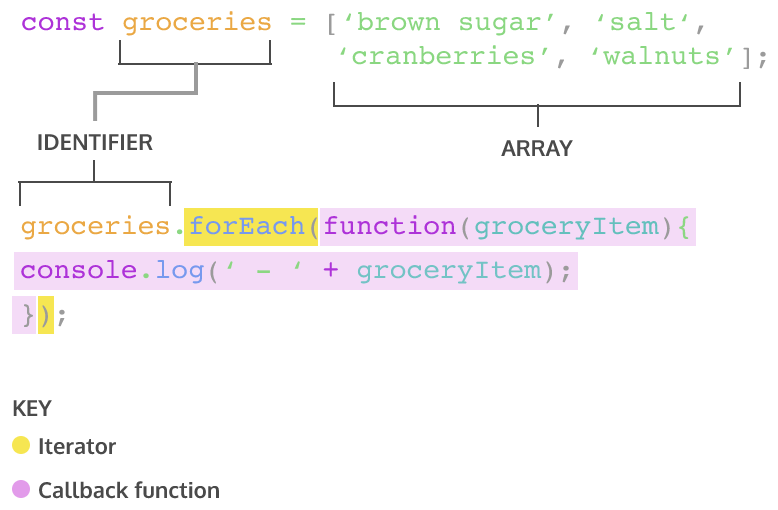
\includegraphics[scale = 0.7]{9_1}
\centering
\end{figure}
The code above will log a nicely formatted list of the groceries to the console. Let us explore the syntax of invoking \colorbox{lightgray}{.forEach()}.
\begin{itemize}[leftmargin = *]
\item \colorbox{lightgray}{groceries.forEach()} calls the \colorbox{lightgray}{forEach} method on the groceries array.
\item \colorbox{lightgray}{.forEach()} takes an argument of callback function. Remember, a callback function is a function passed as an argument into another function.
\item \colorbox{lightgray}{.forEach()} loops through the array and executes the callback function for each element. During each execution, the current element is passed as an argument to the callback function.
\item The return value for \colorbox{lightgray}{.forEach()} will always be \colorbox{lightgray}{undefined}.
\end{itemize}
Another way to pass a callback for \colorbox{lightgray}{.forEach()} is to use arrow function syntax.
\begin{lstlisting}
groceries.forEach(groceryItem => console.log(groceryItem));
\end{lstlisting}
We can also define a function beforehand to be used as the callback function.
\begin{lstlisting}
function printGrocery(element){
  console.log(element);
}

groceries.forEach(printGrocery);
\end{lstlisting}
The above example uses a function declaration but you can also use a function expression or arrow function as well. \\
\newline
All three code snippets do the same thing. In each array iteration method, we can use any of the three examples to supply a callback function as an argument to the iterator. It is good to be aware of the different ways to pass in callback functions as arguments in iterators because developers have different stylistic preferences. Nonetheless, due to the strong adoption of ES6, we will be using arrow function syntax in the later exercises.
\begin{lstlisting}
const fruits = ["mango", "papaya", "pineapple", "apple"];

// Iterate over fruits below
fruits.forEach(item => console.log("I want to eat a " + item));
// Output: 
// I want to eat a mango
// I want to eat a papaya
// I want to eat a pineapple
// I want to eat a apple
\end{lstlisting}



\subsection{The .map() Method} 
The second iterator to cover is \colorbox{lightgray}{.map()}. When \colorbox{lightgray}{.map()} is called on an array, it takes an argument of a callback function and returns a new array! Take a look at an example of calling \colorbox{lightgray}{.map()}:
\begin{lstlisting}
const numbers = [1, 2, 3, 4, 5]; 

const bigNumbers = numbers.map(number => {
  return number * 10;
});
\end{lstlisting}
\colorbox{lightgray}{.map()} works in a similar manner to \colorbox{lightgray}{.forEach()}— the major difference is that \colorbox{lightgray}{.map()} returns a new array.

In the example above:
\begin{itemize}[leftmargin = *]
\item \colorbox{lightgray}{numbers} is an array of numbers.
\item \colorbox{lightgray}{bigNumbers} will store the return value of calling \colorbox{lightgray}{.map()} on \colorbox{lightgray}{numbers}.
\item \colorbox{lightgray}{numbers.map} will iterate through each element in the \colorbox{lightgray}{numbers} array and pass the element into the callback function.
\item \colorbox{lightgray}{return number * 10} is the code we wish to execute upon each element in the array. This will save each value from the \colorbox{lightgray}{numbers} array, multiplied by \colorbox{lightgray}{10}, to a new array.
\end{itemize}
If we take a look at \colorbox{lightgray}{numbers} and \colorbox{lightgray}{bigNumbers}:
\begin{lstlisting}
console.log(numbers); // Output: [1, 2, 3, 4, 5]
console.log(bigNumbers); // Output: [10, 20, 30, 40, 50]
\end{lstlisting}
Notice that the elements in \colorbox{lightgray}{numbers} were not altered and \colorbox{lightgray}{bigNumbers} is a new array.

\subsection{The .filter() Method}
Another useful iterator method is \colorbox{lightgray}{.filter()}. Like \colorbox{lightgray}{.map()}, \colorbox{lightgray}{.filter()} returns a new array. However, \colorbox{lightgray}{.filter()} returns an array of elements after filtering out certain elements from the original array. The callback function for the \colorbox{lightgray}{.filter()} method should return \colorbox{lightgray}{true} or \colorbox{lightgray}{false} depending on the element that is passed to it. The elements that cause the callback function to return \colorbox{lightgray}{true} are added to the new array. Take a look at the following example:
\begin{lstlisting}
const words = ["chair", "music", "pillow", "brick", "pen", "door"]; 

const shortWords = words.filter(word => {
  return word.length < 6;
});
\end{lstlisting}
\begin{itemize}[leftmargin = *]
\item \colorbox{lightgray}{words} is an array that contains string elements.
\item \colorbox{lightgray}{const shortWords =} declares a new variable that will store the returned array from invoking \colorbox{lightgray}{.filter()}.
\item The callback function is an arrow function has a single parameter, \colorbox{lightgray}{word}. Each element in the \colorbox{lightgray}{words} array will be passed to this function as an argument.
\item \colorbox{lightgray}{word.length < 6;} is the condition in the callback function. Any \colorbox{lightgray}{word} from the \colorbox{lightgray}{words} array that has fewer than 6 characters will be added to the \colorbox{lightgray}{shortWords} array.
\end{itemize}
Let’s also check the values of \colorbox{lightgray}{words} and \colorbox{lightgray}{shortWords}:
\begin{lstlisting}
console.log(words); 
// Output: ["chair", "music", "pillow", "brick", "pen", "door"]

console.log(shortWords); 
// Output: ["chair", "music", "brick", "pen", "door"]
\end{lstlisting}
Observe how \colorbox{lightgray}{words} was not mutated, i.e. changed, and \colorbox{lightgray}{shortWords} is a new array.

\subsection{The .findIndex() Method}
We sometimes want to find the location of an element in an array. That is where the \colorbox{lightgray}{.findIndex()} method comes in. Calling \colorbox{lightgray}{.findIndex()} on an array will return the index of the first element that evaluates to \colorbox{lightgray}{true} in the callback function.
\begin{lstlisting}
const jumbledNums = [123, 25, 78, 5, 9]; 

const lessThanTen = jumbledNums.findIndex(num => {
  return num < 10;
});
\end{lstlisting}
\begin{itemize}[leftmargin = *]
\item \colorbox{lightgray}{jumbledNums} is an array that contains elements that are numbers.
\item \colorbox{lightgray}{const lessThanTen =} declares a new variable that stores the returned index number from invoking \colorbox{lightgray}{.findIndex()}.
\item The callback function is an arrow function has a single parameter, \colorbox{lightgray}{num}. Each element in the \colorbox{lightgray}{jumbledNums} array will be passed to this function as an argument.
\item \colorbox{lightgray}{num < 10;} is the condition that elements are checked against. \colorbox{lightgray}{.findIndex()} will return the index of the first element which evaluates to \colorbox{lightgray}{true} for that condition.
\end{itemize}
Let us take a look at what \colorbox{lightgray}{lessThanTen} evaluates to:
\begin{lstlisting}
console.log(lessThanTen); // Output: 3 
\end{lstlisting}
If we check what element has index of 3:
\begin{lstlisting}
console.log(jumbledNums[3]); // Output: 5
\end{lstlisting}
Great, the element in index \colorbox{lightgray}{3} is the number \colorbox{lightgray}{5}. This makes sense since \colorbox{lightgray}{5} is the first element that is less than 10. \\
\newline
If there is not a single element in the array that satisfies the condition in the callback, then \colorbox{lightgray}{.findIndex()} will return \colorbox{lightgray}{-1}.
\begin{lstlisting}
const greaterThan1000 = jumbledNums.findIndex(num => {
  return num > 1000;
});

console.log(greaterThan1000); // Output: -1
\end{lstlisting}

\subsection{The .reduce() Method}
Another widely used iteration method is \colorbox{lightgray}{.reduce()}. The \colorbox{lightgray}{.reduce()} method returns a single value after iterating through the elements of an array, thereby reducing the array. Take a look at the example below:
\begin{lstlisting}
const numbers = [1, 2, 4, 10];

const summedNums = numbers.reduce((accumulator, currentValue) => {
  return accumulator + currentValue
})

console.log(summedNums) // Output: 17
\end{lstlisting}
Here are the values of \colorbox{lightgray}{accumulator} and \colorbox{lightgray}{currentValue} as we iterate through the numbers array:
\begin{center}
\rowcolors{2}{white}{yellow}
\begin{tabular}[H]{ |c|c|c|c| } 
 \hline
 Iteration & \colorbox{lightgray}{accumulator} & \colorbox{lightgray}{currentValue} & return value \\ 
 \hline
 First & 1 & 2 & 3 \\ 
 \hline
 Second & 3 & 4 & 7\\ 
 \hline
 Third & 7 & 10 & 17\\
 \hline
\end{tabular}
\end{center}

Now let us go over the use of \colorbox{lightgray}{.reduce()} from the example above:
\begin{itemize}[leftmargin = *]
\item \colorbox{lightgray}{numbers} is an array that contains numbers.
\item \colorbox{lightgray}{summedNums} is a variable that stores the returned value of invoking \colorbox{lightgray}{.reduce()} on numbers.
\item \colorbox{lightgray}{numbers.reduce()} calls the \colorbox{lightgray}{.reduce()} method on the \colorbox{lightgray}{numbers} array and takes in a callback function as argument.
\item The callback function has two parameters, \colorbox{lightgray}{accumulator} and \colorbox{lightgray}{currentValue}. The value of \colorbox{lightgray}{accumulator} starts off as the value of the first element in the array and the \colorbox{lightgray}{currentValue} starts as the second element. To see the value of \colorbox{lightgray}{accumulator} and \colorbox{lightgray}{currentValue} change, review the chart above.
\item As \colorbox{lightgray}{.reduce()} iterates through the array, the return value of the callback function becomes the \colorbox{lightgray}{accumulator} value for the next iteration, \colorbox{lightgray}{currentValue} takes on the value of the current element in the looping process.
\end{itemize}
The \colorbox{lightgray}{.reduce()} method can also take an optional second parameter to set an initial value for \colorbox{lightgray}{accumulator} (remember, the first argument is the callback function). For instance:
\begin{lstlisting}
const numbers = [1, 2, 4, 10];

const summedNums = numbers.reduce((accumulator, currentValue) => {
  return accumulator + currentValue
}, 100)  // <- Second argument for .reduce()

console.log(summedNums); // Output: 117
\end{lstlisting}
Here is an updated chart that accounts for the second argument of \colorbox{lightgray}{100}:

\begin{center}
\rowcolors{2}{white}{yellow}
\begin{tabular}[H]{ |c|c|c|c| } 
 \hline
 Iteration & \colorbox{lightgray}{accumulator} & \colorbox{lightgray}{currentValue} & return value \\ 
 \hline
 First & 100 & 1 & 101 \\ 
 \hline
 Second & 101 & 2 & 103\\ 
 \hline
 Third & 103 & 4 & 107\\
 \hline
 Fourth & 107 & 10 & 17 \\
 \hline
\end{tabular}
\end{center}

\subsection{Iterator Documentation}
There are many additional built-in array methods, a complete list of which is on the 
\href{https://developer.mozilla.org/en-US/docs/Web/JavaScript/Reference/Global_Objects/Array}{MDN’s Array iteration methods page}.
The documentation for each method contains several sections:
\begin{enumerate}[leftmargin = *]
\item A short definition.
\item A block with the correct syntax for using the method.
\item A list of parameters the method accepts or requires.
\item The return value of the function.
\item An extended description.
\item Examples of the method’s use.
\item Other additional information.
\end{enumerate}

\subsection{More Iterators}
Let us briefly learn two other popular iterators. Below we will explore \colorbox{lightgray}{some()} and \colorbox{lightgray}{every()}.
\subsubsection{The .some() Method}
The \colorbox{lightgray}{some()} method tests whether at least one element in the array passes the test implemented by the provided function. It returns a Boolean value.
\begin{lstlisting}
const array = [1, 2, 3, 4, 5];

// checks whether an element is even
const even = (element) => element % 2 === 0;

console.log(array.some(even)); // Output: true
\end{lstlisting}

\subsubsection{The .every() Method}
The \colorbox{lightgray}{every()} method tests whether all elements in the array pass the test implemented by the provided function. It returns a Boolean value.
\begin{lstlisting}
const isBelowThreshold = (currentValue) => currentValue < 40;

const array1 = [1, 30, 39, 29, 10, 13];

console.log(array1.every(isBelowThreshold)); // Output: true
\end{lstlisting}

\subsection{Review}
We have learned a number of useful methods in this chapter as well as how to use the JavaScript documentation from the Mozilla Developer Network to discover and understand additional methods. 
\begin{itemize}[leftmargin = *]
\item \colorbox{lightgray}{.forEach()} is used to execute the same code on every element in an array but does not change the array and returns undefined.
\item \colorbox{lightgray}{.map()} executes the same code on every element in an array and returns a new array with the updated elements.
\item \colorbox{lightgray}{.filter()} checks every element in an array to see if it meets certain criteria and returns a new array with the elements that return truthy for the criteria.
\item \colorbox{lightgray}{.findIndex()} returns the index of the first element of an array which satisfies a condition in the callback function. It returns -1 if none of the elements in the array satisfies the condition.
\item \colorbox{lightgray}{.reduce()} iterates through an array and takes the values of the elements and returns a single value.
\item All iterator methods takes a callback function that can be pre-defined, or a function expression, or an arrow function.
\item You can visit the \href{https://developer.mozilla.org/en-US/docs/Web/JavaScript/Reference/Global_Objects/Array}{Mozilla Developer Network} to learn more about iterator methods (and all other parts of JavaScript!).
\end{itemize}

\newpage
\section{Objects}
\subsection{Introduction to Objects}
It is time to learn more about the basic structure that permeates nearly every aspect of JavaScript programming: objects. \\
\newline
You are probably already more comfortable with objects than you think, because JavaScript loves objects. Many components of the language are actually objects under the hood, and even the parts that are not— like strings or numbers— can still act like objects in some instances. \\
\newline
There are only seven fundamental data types in JavaScript, and six of those are the primitive data types: string, number, boolean, null, undefined, and symbol. With the seventh type, objects, we open our code to more complex possibilities. We can use JavaScript objects to model real-world things, like a basketball, or we can use objects to build the data structures that make the web possible. \\
\newline
At their core, JavaScript objects are containers storing related data and functionality, but that deceptively simple task is extremely powerful in practice. You have been using the power of objects all along, but now it is time to understand the mechanics of objects and start making your own.

\subsection{Creating Object Literals} 
Objects can be assigned to variables just like any JavaScript type. We use curly braces, \colorbox{lightgray}{\{\}}, to designate an \textit{object literal}:
\begin{lstlisting}
let spaceship = {}; // spaceship is an empty object
\end{lstlisting}
We fill an object with unordered data. This data is organized into \textit{key-value pairs}. A key is like a variable name that points to a location in memory that holds a value. A key’s value can be of any data type in the language including functions or other objects. \\
\newline
We make a key-value pair by writing the key’s name, or \textit{identifier}, followed by a colon and then the value. We separate each key-value pair in an object literal with a comma (\colorbox{lightgray}{,}). Keys are strings, but when we have a key that does not have any special characters in it, JavaScript allows us to omit the quotation marks:
\begin{figure}[H]
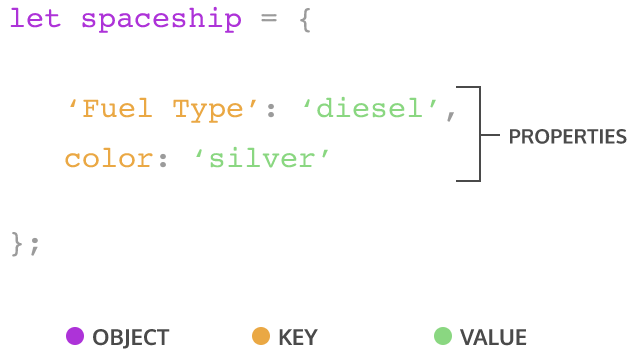
\includegraphics[scale = 0.65]{10_1}
\centering 
\end{figure}
\newpage
\begin{lstlisting}
// An object literal with two key-value pairs
let spaceship = {
  "Fuel Type": "diesel",
  color: "silver"
};
\end{lstlisting}
The \colorbox{lightgray}{spaceship} object has two properties \colorbox{lightgray}{Fuel Type} and \colorbox{lightgray}{color}. \colorbox{lightgray}{`Fuel Type'} has quotation marks because it contains a space character.

\subsection{Accessing Properties}
There are two ways we can access an object’s property. Let us explore the first way— dot notation, \colorbox{lightgray}{.}. \\
\newline
You have used dot notation to access the properties and methods of built-in objects and data instances:
\begin{lstlisting}
"hello".length; // Returns 5
\end{lstlisting}
With property dot notation, we write the object’s name, followed by the dot operator and then the property name (key): 
\begin{lstlisting}
let spaceship = {
  homePlanet: "Earth",
  color: "silver"
};
spaceship.homePlanet; // Returns "Earth",
spaceship.color; // Returns "silver",
\end{lstlisting}
\begin{figure}[H]
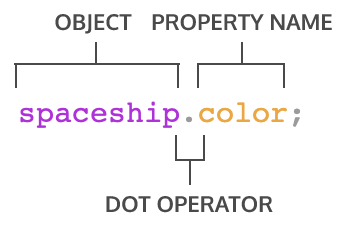
\includegraphics[scale = 0.7]{10_2}
\centering
\end{figure}
If we try to access a property that does not exist on that object, \colorbox{lightgray}{undefined} will be returned.
\begin{lstlisting}
spaceship.favoriteIcecream; // Returns undefined
\end{lstlisting}

\subsection{Bracket Notation}
The second way to access a key’s value is by using bracket notation, \colorbox{lightgray}{$[$ $]$}. You have used bracket notation when indexing an array:
\begin{lstlisting}
["A", "B", "C"][0]; // Returns "A"
\end{lstlisting}
To use bracket notation to access an object’s property, we pass in the property name (key) as a string.
\begin{figure}[H]
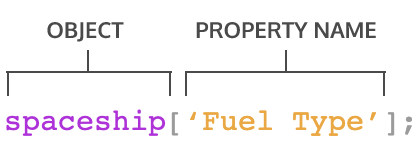
\includegraphics[scale = 0.7]{10_3}
\centering
\end{figure}
We \textbf{must} use bracket notation when accessing keys that have numbers, spaces, or special characters in them. Without bracket notation in these situations, our code would throw an error.
\begin{lstlisting}
let spaceship = {
  "Fuel Type": "Turbo Fuel",
  "Active Duty": true,
  homePlanet: "Earth",
  numCrew: 5
};
spaceship["Active Duty"];   // Returns true
spaceship["Fuel Type"];   // Returns  "Turbo Fuel"
spaceship["numCrew"];   // Returns 5
spaceship["!!!!!!!!!!!!!!!"];   // Returns undefined
\end{lstlisting}
With bracket notation you can also use a variable inside the brackets to select the keys of an object. This can be especially helpful when working with functions:
\begin{lstlisting}
let returnAnyProp = (objectName, propName) => objectName[propName];

returnAnyProp(spaceship, "homePlanet"); // Returns "Earth"
\end{lstlisting}
If we tried to write our \colorbox{lightgray}{returnAnyProp()} function with dot notation (\colorbox{lightgray}{objectName.propName}) the computer would look for a key of \colorbox{lightgray}{`propName'} on our object and not the value of the \colorbox{lightgray}{propName} parameter.

\subsection{Property Assignment}
Once we have defined an object, we are not stuck with all the properties we wrote. Objects are mutable meaning we can update them after we create them. We can use either dot notation, \colorbox{lightgray}{.}, or bracket notation, \colorbox{lightgray}{$[$ $]$}, and the assignment operator, \colorbox{lightgray}{=} to add new key-value pairs to an object or change an existing property.
\begin{figure}[H]
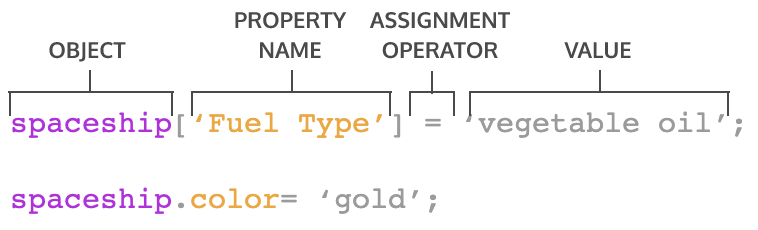
\includegraphics[scale = 0.68]{10_4}
\centering
\end{figure}
One of two things can happen with property assignment:
\begin{itemize}[leftmargin = *]
\item If the property already exists on the object, whatever value it held before will be replaced with the newly assigned value.
\item If there was no property with that name, a new property will be added to the object.
\end{itemize}
It is important to know that although we cannot reassign an object declared with \colorbox{lightgray}{const}, we can still mutate it, meaning we can add new properties and change the properties that are there. 
\begin{lstlisting}
const spaceship = {type: "shuttle"};
spaceship = {type: "alien"}; // TypeError: Assignment to constant variable.
spaceship.type = "alien"; // Changes the value of the type property
spaceship.speed = "Mach 5"; 
// Creates a new key of "speed" with a value of "Mach 5"
\end{lstlisting}
You can delete a property from an object with the \colorbox{lightgray}{delete} operator.
\begin{lstlisting}
const spaceship = {
  "Fuel Type": "Turbo Fuel",
  homePlanet: "Earth",
  mission: "Explore the universe"
};

delete spaceship.mission;  // Removes the mission property
\end{lstlisting}

\subsection{Methods}
When the data stored on an object is a function we call that a \textit{method}. A property is what an object has, while a method is what an object does. Object methods seem familiar because we have been using them all along. For example \colorbox{lightgray}{console} is a global javascript object and \colorbox{lightgray}{.log()} is a method on that object. \colorbox{lightgray}{Math} is also a global javascript object and \colorbox{lightgray}{.floor()} is a method on it. \\
\newline
We can include methods in our object literals by creating ordinary, comma-separated key-value pairs. The key serves as our method’s name, while the value is an anonymous function expression.
\begin{lstlisting}
const alienShip = {
  invade: function () { 
    console.log("Hello! We have come to dominate your planet.")
  }
};
\end{lstlisting}
With the new method syntax introduced in ES6 we can omit the colon and the \colorbox{lightgray}{function} keyword.
\begin{lstlisting}
const alienShip = {
  invade () { 
    console.log("Hello! We have come to dominate your planet.")
  }
};
\end{lstlisting}
Object methods are invoked by appending the object’s name with the dot operator followed by the method name and parentheses:
\begin{lstlisting}
alienShip.invade(); // Prints "Hello! We have come to dominate your planet."
\end{lstlisting}

\subsection{Nested Objects}
In application code, objects are often nested— an object might have another object as a property which in turn could have a property that is an array of even more objects. \\
\newline
In our \colorbox{lightgray}{spaceship} object, we want a \colorbox{lightgray}{crew} object. This will contain all the crew members who do important work on the craft. Each of those \colorbox{lightgray}{crew} members are objects themselves. They have properties like \colorbox{lightgray}{name}, and \colorbox{lightgray}{degree}, and they each have unique methods based on their roles. We can also nest other objects in the \colorbox{lightgray}{spaceship} such as a \colorbox{lightgray}{telescope} or nest details about the spaceship’s computers inside a parent \colorbox{lightgray}{nanoelectronics} object. 
\begin{lstlisting}
const spaceship = {
     telescope: {
        yearBuilt: 2018,
        model: "91031-XLT",
        focalLength: 2032 
     },
    crew: {
        captain: { 
            name: "Sandra", 
            degree: "Computer Engineering", 
            encourageTeam() { console.log("We got this!") } 
         }
    },
    engine: {
        model: "Nimbus2000"
     },
     nanoelectronics: {
         computer: {
            terabytes: 100,
            monitors: "HD"
         },
        "back-up": {
           battery: "Lithium",
           terabytes: 50
         }
    }
}; 
\end{lstlisting}
We can chain operators to access nested properties. We will have to pay attention to which operator makes sense to use in each layer. It can be helpful to pretend you are the computer and evaluate each expression from left to right so that each operation starts to feel a little more manageable.
\begin{lstlisting}
spaceship.nanoelectronics["back-up"].battery; // Returns "Lithium"
\end{lstlisting}
In the preceding code:
\begin{itemize}[leftmargin = *]
\item First the computer evaluates \colorbox{lightgray}{spaceship.nanoelectronics}, which results in an object containing the \colorbox{lightgray}{back-up} and \colorbox{lightgray}{computer} objects.
\item We accessed the \colorbox{lightgray}{back-up} object by appending \colorbox{lightgray}{["back-up"]}.
\item The \colorbox{lightgray}{back-up} object has a battery property, accessed with \colorbox{lightgray}{.battery} which returned the value stored there: \colorbox{lightgray}{"Lithium"}. 
\end{itemize}

\subsection{Pass By Reference}
Objects are \textit{passed by reference}. This means when we pass a variable assigned to an object into a function as an argument, the computer interprets the parameter name as pointing to the space in memory holding that object. As a result, functions which change object properties actually mutate the object permanently (even when the object is assigned to a \colorbox{lightgray}{const} variable).
\begin{lstlisting}
const spaceship = {
  homePlanet : "Earth",
  color : "silver"
};

let paintIt = obj => {
  obj.color = "glorious gold"
};

paintIt(spaceship);

spaceship.color // Returns "glorious gold"
\end{lstlisting}
Our function \colorbox{lightgray}{paintIt()} permanently changed the color of our \colorbox{lightgray}{spaceship} object. However, reassignment of the \colorbox{lightgray}{spaceship} variable would not work in the same way:
\begin{lstlisting}
let spaceship = {
  homePlanet : "Earth",
  color : "red"
};
let tryReassignment = obj => {
  obj = {
    identified : false, 
    "transport type": "flying"
  }
  console.log(obj) // Prints {"identified": false, "transport type": "flying"}
};
tryReassignment(spaceship) // The attempt at reassignment does not work.
spaceship // Still returns {homePlanet : "Earth", color : "red"};

spaceship = {
  identified : false, 
  "transport type": "flying"
}; // Regular reassignment still works.
\end{lstlisting}
Let us look at what happened in the code example:
\begin{itemize}[leftmargin = *]
\item We declared this \colorbox{lightgray}{spaceship} object with \colorbox{lightgray}{let}. This allowed us to reassign it to a new object with \colorbox{lightgray}{identified} and \colorbox{lightgray}{'transport type'} properties with no problems.
\item When we tried the same thing using a function designed to reassign the object passed into it, the reassignment didn’t stick (even though calling \colorbox{lightgray}{console.log()} on the object produced the expected result).
\item When we passed \colorbox{lightgray}{spaceship} into that function, \colorbox{lightgray}{obj} became a reference to the memory location of the spaceship object, but \textit{not} to the \colorbox{lightgray}{spaceship} variable. This is because the \colorbox{lightgray}{obj} parameter of the \colorbox{lightgray}{tryReassignment()} function is a variable in its own right. The body of \colorbox{lightgray}{tryReassignment()} has no knowledge of the spaceship variable at all!
\item When we did the reassignment in the body of \colorbox{lightgray}{tryReassignment()}, the \colorbox{lightgray}{obj} variable came to refer to the memory location of the object \colorbox{lightgray}{\{`identified' : false, `transport type' : `flying'\}}, while the \colorbox{lightgray}{spaceship} variable was completely unchanged from its earlier value.
\end{itemize}

\subsection{Looping Through Objects}
Loops are programming tools that repeat a block of code until a condition is met. We learned how to iterate through arrays using their numerical indexing, but the key-value pairs in objects are not ordered. \href{https://developer.mozilla.org/en-US/docs/Web/JavaScript/Reference/Statements/for...in}{JavaScript has given us alternative solution for iterating through objects with the \colorbox{lightgray}{for...in} syntax}. \\
\newline
\colorbox{lightgray}{for...in} will execute a given block of code for each property in an object. 
\begin{lstlisting}
let spaceship = {
    crew: {
    captain: { 
        name: "Lily", 
        degree: "Computer Engineering", 
        cheerTeam() { console.log("You got this!") } 
        },
    "chief officer": { 
        name: "Dan", 
        degree: "Aerospace Engineering", 
        agree() { console.log("I agree, captain!") } 
        },
    medic: { 
        name: "Clementine", 
        degree: "Physics", 
        announce() { console.log("Jets on!") } },
    translator: {
        name: "Shauna", 
        degree: 'Conservation Science', 
        powerFuel() { console.log("The tank is full!") } 
        }
    }
}; 
// for...in
for (let crewMember in spaceship.crew) {
  console.log{(*@\texttt{\textasciigrave}@*)${crewMember}: ${spaceship.crew[crewMember].name}(*@\texttt{\textasciigrave}@*))
};
\end{lstlisting}
Our \colorbox{lightgray}{for...in} will iterate through each element of the \colorbox{lightgray}{spaceship.crew} object. In each iteration, the variable \colorbox{lightgray}{crewMember} is set to one of \colorbox{lightgray}{spaceship.crew}'s keys, enabling us to log a list of crew members’ role and \colorbox{lightgray}{name}.

\subsection{Review}
Let us review what we learned in this chapter:
\begin{itemize}[leftmargin = *]
\item Objects store collections of \textit{key-value} pairs.
\item Each key-value pair is a property—when a property is a function it is known as a method.
\item An object literal is composed of comma-separated key-value pairs surrounded by curly braces.
\item You can access, add or edit a property within an object by using dot notation or bracket notation.
\item We can add methods to our object literals using key-value syntax with anonymous function expressions as values or by using the new ES6 method syntax.
\item We can navigate complex, nested objects by chaining operators.
\item Objects are mutable—we can change their properties even when they are declared with \colorbox{lightgray}{const}.
\item Objects are passed by reference— when we make changes to an object passed into a function, those changes are permanent.
\item We can iterate through objects using the \colorbox{lightgray}{For...in} syntax.
\end{itemize}

\newpage
\section{Advanced Objects}
\subsection{Advanced Objects Introduction}
Remember, objects in JavaScript are containers that store data and functionality. In this lesson, we will build upon the fundamentals of creating objects and explore some advanced concepts.
In this chapter we will learn to:
\begin{itemize}[leftmargin = *]
\item use the \colorbox{lightgray}{this} keyword.
\item convey privacy in JavaScript methods.
\item define getters and setters in objects.
\item create factory functions.
\item use destructuring techniques.
\end{itemize}

\subsection{The this Keyword}
Objects are collections of related data and functionality. We store that functionality in methods on our objects:
\begin{lstlisting}
const goat = {
  dietType: "herbivore",
  makeSound() {
    console.log("baaa");
  }
};
\end{lstlisting}
In our \colorbox{lightgray}{goat} object we have a \colorbox{lightgray}{.makeSound()} method. We can invoke the \colorbox{lightgray}{.makeSound()} method on \colorbox{lightgray}{goat}.
\begin{lstlisting}
goat.makeSound(); // Prints baaa
\end{lstlisting}
We have a \colorbox{lightgray}{goat} object that can print \colorbox{lightgray}{baaa} to the console. What if we wanted to add a new method to our \colorbox{lightgray}{goat} object called \colorbox{lightgray}{.diet()} that prints the goat's \colorbox{lightgray}{dietType}?
\begin{lstlisting}
const goat = {
  dietType: "herbivore",
  makeSound() {
    console.log("baaa");
  },
  diet() {
    console.log(dietType);
  }
};
goat.diet(); 
// Output will be "ReferenceError: dietType is not defined"
\end{lstlisting}
That is strange, why is \colorbox{lightgray}{dietType} not defined even though it is a property of \colorbox{lightgray}{goat}? That is because inside the scope of the \colorbox{lightgray}{.diet()} method, we do not automatically have access to other properties of the \colorbox{lightgray}{goat} object. Here is where the \colorbox{lightgray}{this} keyword comes to the rescue. If we change the \colorbox{lightgray}{.diet()} method to use the \colorbox{lightgray}{this}, the \colorbox{lightgray}{.diet()} works. 
\begin{lstlisting}
const goat = {
  dietType: "herbivore",
  makeSound() {
    console.log("baaa");
  },
  diet() {
    console.log(this.dietType);
  }
};

goat.diet(); // Output: herbivore
\end{lstlisting}
The \colorbox{lightgray}{this} keyword references the \textit{calling object} which provides access to the calling object’s properties. In the example above, the calling object is \colorbox{lightgray}{goat} and by using \colorbox{lightgray}{this} we are accessing the \colorbox{lightgray}{goat} object itself, and then the \colorbox{lightgray}{dietType} property of \colorbox{lightgray}{goat} by using property dot notation.

\subsection{Arrow Functions and this}
We saw in the previous exercise that for a method, the calling object is the object the method belongs to. If we use the \colorbox{lightgray}{this} keyword in a method then the value of \colorbox{lightgray}{this} is the calling object. However, it becomes more complicated when we start using arrow functions for methods. Take a look at the example below:
\begin{lstlisting}
const goat = {
  dietType: "herbivore",
  makeSound() {
    console.log("baaa");
  },
  diet: () => {
    console.log(this.dietType);
  }
};

goat.diet(); // Prints undefined
\end{lstlisting}
In the comment, you can see that \colorbox{lightgray}{goat.diet()} would log \colorbox{lightgray}{undefined}. What happened? Notice that in the \colorbox{lightgray}{.diet()} is defined using an arrow function. \\
\newline
Arrow functions inherently \textit{bind}, or tie, an already defined \colorbox{lightgray}{this} value to the function itself that is NOT the calling object. In the code snippet above, the value of \colorbox{lightgray}{this} is the global object, or an object that exists in the \textit{global scope}, which does not have a \colorbox{lightgray}{dietType} property and therefore returns \colorbox{lightgray}{undefined}. \\
\newline
To read more about either arrow functions or the global object check out the MDN documentation of \href{https://developer.mozilla.org/en-US/docs/Glossary/Global_object}{the global object} and \href{https://developer.mozilla.org/en-US/docs/Web/JavaScript/Reference/Functions/Arrow_functions}{arrow functions}. \\
\newline
The key takeaway from the example above is to \textit{avoid} using arrow functions when using \colorbox{lightgray}{this} in a method!

\subsection{Privacy}
Accessing and updating properties is fundamental in working with objects. However, there are cases in which we don’t want other code simply accessing and updating an object’s properties. When discussing \textit{privacy} in objects, we define it as the idea that only certain properties should be mutable or able to change in value. \\
\newline
Certain languages have privacy built-in for objects, but JavaScript does not have this feature. Rather, JavaScript developers follow naming conventions that signal to other developers how to interact with a property. One common convention is to place an underscore \colorbox{lightgray}{\_} before the name of a property to mean that the property should not be altered. Here’s an example of using \colorbox{lightgray}{\_} to prepend a property.
\begin{lstlisting}
const bankAccount = {
  _amount: 1000
}
\end{lstlisting}
In the example above, the \colorbox{lightgray}{\_amount} is not intended to be directly manipulated. Even so, it is still possible to reassign \colorbox{lightgray}{\_amount}:
\begin{lstlisting}
bankAccount._amount = 1000000;
\end{lstlisting}
%\colorbox{black!85}{\makebox[0.5em]{\strut\textcolor{white}{\_}}}
Later, we will cover the use of methods called \textit{getters} and \textit{setters}. Both methods are used to respect the intention of properties prepended, or began, with \colorbox{lightgray}{\_}. Getters can return the value of internal properties and setters can safely reassign property values. 

\subsection{Getters}
\textit{Getters} are methods that get and return the internal properties of an object. But they can do more than just retrieve the value of a property. Let us take a look at a getter method:
\begin{lstlisting}
const person = {
  _firstName: "John",
  _lastName: "Doe",
  get fullName() {
    if (this._firstName && this._lastName){
      return (*@\texttt{\textasciigrave}@*)${this._firstName} ${this._lastName}(*@\texttt{\textasciigrave}@*);
    } else {
      return "Missing a first name or a last name.";
    }
  }
}

// To call the getter method: 
person.fullName; // 'John Doe'
\end{lstlisting}
Notice that in the getter method above:
\begin{itemize}[leftmargin = *]
\item We use the \colorbox{lightgray}{get} keyword followed by a function.
\item We use an \colorbox{lightgray}{if...else} conditional to check if both \colorbox{lightgray}{\_firstName} and \colorbox{lightgray}{\_lastName} exist (by making sure they both return truthy values) and then return a different value depending on the result.
\item We can access the calling object’s internal properties using \colorbox{lightgray}{this}. In \colorbox{lightgray}{fullName}, we are accessing both \colorbox{lightgray}{this.\_firstName} and \colorbox{lightgray}{this.\_lastName}.
\item In the last line we call \colorbox{lightgray}{fullName} on \colorbox{lightgray}{person}. In general, getter methods do not need to be called with a set of parentheses. Syntactically, it looks like we are accessing a property.
\end{itemize}
Now that we have gone over syntax, let’s discuss some notable advantages of using getter methods:
\begin{itemize}[leftmargin = *]
\item Getters can perform an action on the data when getting a property.
\item Getters can return different values using conditionals.
\item In a getter, we can access the properties of the calling object using \colorbox{lightgray}{this}.
\item The functionality of our code is easier for other developers to understand.
\end{itemize}
Another thing to keep in mind when using getter (and setter) methods is that properties cannot share the same name as the getter/setter function. If we do so, then calling the method will result in an infinite call stack error. One workaround is to add an underscore before the property name like we did in the example above.

\subsection{Setters}
Along with getter methods, we can also create \textit{setter} methods which reassign values of existing properties within an object. Let us see an example of a setter method:
\begin{lstlisting}
const person = {
  _age: 37,
  set age(newAge){
    if (typeof newAge === "number"){
      this._age = newAge;
    } else {
      console.log("You must assign a number to age");
    }
  }
};
\end{lstlisting}
Notice that in the example above:
\begin{itemize}[leftmargin = *]
\item We can perform a check for what value is being assigned to \colorbox{lightgray}{this.\_age}.
\item When we use the setter method, only values that are numbers will reassign \colorbox{lightgray}{this.\_age}.
\item There are different outputs depending on what values are used to reassign \colorbox{lightgray}{this.\_age}.
\end{itemize}
Then to use the setter method:
\begin{lstlisting}
person.age = 40;
console.log(person._age); // Logs: 40
person.age = "40"; // Logs: You must assign a number to age
\end{lstlisting}
Setter methods like \colorbox{lightgray}{age} do not need to be called with a set of parentheses. Syntactically, it looks like we are reassigning the value of a property. \\
\newline
Like getter methods, there are similar advantages to using setter methods that include checking input, performing actions on properties, and displaying a clear intention for how the object is supposed to be used. Nonetheless, even with a setter method, it is still possible to directly reassign properties. For example, in the example above, we can still set \colorbox{lightgray}{.\_age} directly: 
\begin{lstlisting}
person._age = "forty-five"
console.log(person._age); // Prints forty-five
\end{lstlisting}

\subsection{Factory Functions}
So far we have been creating objects individually, but there are times where we want to create many instances of an object quickly. Here is where factory functions come in. A real world factory manufactures multiple copies of an item quickly and on a massive scale. A factory function is a function that returns an object and can be reused to make multiple object instances. Factory functions can also have parameters allowing us to customize the object that gets returned. \\
\newline
Let us say we wanted to create an object to represent monsters in JavaScript. There are many different types of monsters and we could go about making each monster individually but we can also use a factory function to make our lives easier. To achieve this diabolical plan of creating multiple monsters objects, we can use a factory function that has parameters: 
\begin{lstlisting}
const monsterFactory = (name, age, energySource, catchPhrase) => {
  return { 
    name: name,
    age: age, 
    energySource: energySource,
    scare() {
      console.log(catchPhrase);
    } 
  }
};
\end{lstlisting}
In the \colorbox{lightgray}{monsterFactory} function above, it has four parameters and returns an object that has the properties: \colorbox{lightgray}{name}, \colorbox{lightgray}{age}, \colorbox{lightgray}{energySource}, and \colorbox{lightgray}{scare()}. To make an object that represents a specific monster like a ghost, we can call \colorbox{lightgray}{monsterFactory} with the necessary arguments and assign the return value to a variable:
\begin{lstlisting}
const ghost = monsterFactory("Ghouly", 251, "ectoplasm", "BOO!");
ghost.scare(); // "BOO!"
\end{lstlisting}
Now we have a \colorbox{lightgray}{ghost} object as a result of calling \colorbox{lightgray}{monsterFactory()} with the needed arguments. With \colorbox{lightgray}{monsterFactory} in place, we do not have to create an object literal every time we need a new monster. Instead, we can invoke the \colorbox{lightgray}{monsterFactory} function with the necessary arguments to make a monster. 

\subsection{Property Value Shorthand}
ES6 introduced some new shortcuts for assigning properties to variables known as \textit{destructuring}. \\
\newline
In the previous chapter, we created a factory function that helped us create objects. We had to assign each property a key and value even though the key name was the same as the parameter name we assigned to it. To remind ourselves, here is a truncated version of the factory function:
\begin{lstlisting}
const monsterFactory = (name, age) => {
  return { 
    name: name,
    age: age
  }
};
\end{lstlisting}
Imagine if we had to include more properties, that process would quickly become tedious. But we can use a destructuring technique, called \textit{property value shorthand}, to save ourselves some keystrokes. The example below works exactly like the example above: 
\begin{lstlisting}
const monsterFactory = (name, age) => {
  return { 
    name,
    age 
  }
};
\end{lstlisting}
Notice that we do not have to repeat ourselves for property assignments. 

\subsection{Destructured Assignment}
We often want to extract key-value pairs from objects and save them as variables. Take for example the following object:
\begin{lstlisting}
const vampire = {
  name: "Dracula",
  residence: "Transylvania",
  preferences: {
    day: "stay inside",
    night: "satisfy appetite"
  }
};
\end{lstlisting}
If we wanted to extract the \colorbox{lightgray}{residence} property as a variable, we could using the following code:
\begin{lstlisting}
const residence = vampire.residence; 
console.log(residence); // Prints "Transylvania"
\end{lstlisting}
However, we can also take advantage of a destructuring technique called \textit{destructured assignment} to save ourselves some keystrokes. In destructured assignment we create a variable with the name of an object’s key that is wrapped in curly braces \colorbox{lightgray}{\{ \}} and assign to it the object. Take a look at the example below:
\begin{lstlisting}
const { residence } = vampire; 
console.log(residence); // Prints "Transylvania"
\end{lstlisting}
Look back at the \colorbox{lightgray}{vampire} object’s properties in the first code example. Then, in the example above, we declare a new variable \colorbox{lightgray}{residence} that extracts the value of the \colorbox{lightgray}{residence} property of \colorbox{lightgray}{vampire}. When we log the value of \colorbox{lightgray}{residence} to the console, \colorbox{lightgray}{`Transylvania'} is printed. \\
\newline
We can even use destructured assignment to grab nested properties of an object: 
\begin{lstlisting}
const { day } = vampire.preferences; 
console.log(day); // Prints "stay inside"
\end{lstlisting}
Variables created by destructured assignment references the object directly. 
\begin{lstlisting}
const robot = {
  functionality: {
    beep() {
      console.log("Beep Boop");
    },
  }
};
const { functionality } = robot; 
functionality.beep(); \\Output: Beep Boop
\end{lstlisting}
Since \colorbox{lightgray}{functionality} is referencing \colorbox{lightgray}{robot.functionality}, we can call the methods available to \colorbox{lightgray}{robot.functionality} simply through \colorbox{lightgray}{functionality}.

\subsection{Built-in Object Methods}
Previously, we have been creating instances of objects that have their own methods. But, we can also take advantage of built-in methods for Objects. For example, we have access to object instance methods like: \colorbox{lightgray}{.hasOwnProperty()}, \colorbox{lightgray}{.valueOf()}, and many others. Check out: \href{https://developer.mozilla.org/en-US/docs/Web/JavaScript/Reference/Global_Objects/Object#Methods}{MDN’s object instance documentation}. \\
\newline
There are also useful Object class methods such as \colorbox{lightgray}{Object.assign()}, \colorbox{lightgray}{Object.entries()}, and \colorbox{lightgray}{Object.keys()} just to name a few. For a comprehensive list, browse: \href{https://developer.mozilla.org/en-US/docs/Web/JavaScript/Reference/Global_Objects/Object#Methods_of_the_Object_constructor}{MDN’s object instance documentation}. \\
\newline
Below we will explore \colorbox{lightgray}{Object.keys()}, \colorbox{lightgray}{Object.entries()}, and \colorbox{lightgray}{Object.assign()}. 
\subsubsection{The Object.keys() Method}
The \colorbox{lightgray}{Object.keys()} method returns an array of a given object's own enumerable property \textbf{names}, iterated in the same order that a normal loop would.
\begin{lstlisting}
const object1 = {
  a: "somestring",
  b: 42,
  c: false
};

console.log(Object.keys(object1)); // Output: Array ["a", "b", "c"]
\end{lstlisting}

\subsubsection{The Object.entries() Method}
The \colorbox{lightgray}{Object.entries()} method returns an array of a given object's own enumerable string-keyed property \colorbox{lightgray}{[key, value]} pairs, in the same order as that provided by a \colorbox{lightgray}{for...in} loop. (The only important difference is that a \colorbox{lightgray}{for...in} loop enumerates properties in the prototype chain as well). \\
\newline 
The order of the array returned by \colorbox{lightgray}{Object.entries()} does not depend on how an object is defined. If there is a need for certain ordering, then the array should be sorted first. \\ Like \colorbox{lightgray}{Object.entries(obj).sort((a, b) => b[0].localeCompare(a[0]));}.
\begin{lstlisting}
const object1 = {
  a: "somestring",
  b: 42
};

for (const [key, value] of Object.entries(object1)) {
  console.log((*@\texttt{\textasciigrave}@*)${key}: ${value}(*@\texttt{\textasciigrave}@*));
}

// Output:
// "a: somestring"
// "b: 42"
// order is not guaranteed
\end{lstlisting}

\subsubsection{The Object.assign() Method}
The \colorbox{lightgray}{Object.assign()} method copies all enumerable own properties from one or more source objects to a target object. It returns the target object.
\begin{lstlisting}
const target = { a: 1, b: 2 };
const source = { b: 4, c: 5 };

const returnedTarget = Object.assign(target, source);

console.log(target); // Output: Object { a: 1, b: 4, c: 5 }

console.log(returnedTarget); // Output: Object { a: 1, b: 4, c: 5 }
\end{lstlisting}

\subsection{Review}
\begin{itemize}[leftmargin = *]
\item The object that a method belongs to is called the \textit{calling object}.
\item The \colorbox{lightgray}{this} keyword refers the calling object and can be used to access properties of the calling object.
\item Methods do not automatically have access to other internal properties of the calling object.
\item The value of \colorbox{lightgray}{this} depends on where the \colorbox{lightgray}{this} is being accessed from.
\item We cannot use arrow functions as methods if we want to access other internal properties.
\item JavaScript objects do not have built-in privacy, rather there are conventions to follow to notify other developers about the intent of the code.
\item The usage of an underscore before a property name means that the original developer did not intend for that property to be directly changed.
\item Setters and getter methods allow for more detailed ways of accessing and assigning properties.
\item Factory functions allow us to create object instances quickly and repeatedly.
\item There are different ways to use object destructuring: one way is the property value shorthand and another is destructured assignment.
As with any concept, it is a good skill to learn how to use the documentation with objects.
\end{itemize}

\newpage
\section{Classes}
\subsection{Introduction to Classes}
JavaScript is an \textit{object-oriented programming} (OOP) language we can use to model real-world items. In this chapter, you will learn how to make \textit{classes}. Classes are a tool that developers use to quickly produce similar objects. \\
\newline
Take, for example, an object representing a dog named \colorbox{lightgray}{halley}. This dog’s \colorbox{lightgray}{name} (a key) is \colorbox{lightgray}{"Halley"} (a value) and has an \colorbox{lightgray}{age} (another key) of \colorbox{lightgray}{3} (another value). We create the \colorbox{lightgray}{halley} object below:
\begin{lstlisting}
let halley = {
  _name: "Halley",
  _behavior: 0,

  get name() {
    return this._name;
  },

  get behavior() {
    return this._behavior;
  },

  incrementBehavior() {
    this._behavior++;
  }
}
\end{lstlisting}
Now, imagine you own a dog daycare and want to create a catalog of all the dogs who belong to the daycare. Instead of using the syntax above for every dog that joins the daycare, we can create a \colorbox{lightgray}{Dog} class that serves as a template for creating new \colorbox{lightgray}{Dog} objects. For each new dog, you can provide a value for their name. Afterwards, we will introduce inheritance and static methods — two features that will make your code more efficient and meaningful. 
\begin{lstlisting}
class Dog {
  constructor(name) {
    this._name = name;
    this._behavior = 0;
  }

  get name() {
    return this._name;
  }
  get behavior() {
    return this._behavior;
  }   

  incrementBehavior() {
    this._behavior ++;
  }
}
const halley = new Dog("Halley");
console.log(halley.name); // Print name value to console
console.log(halley.behavior); // Print behavior value to console
\end{lstlisting}

\subsection{Constructor}
Previously, we saw the creation of a class called \colorbox{lightgray}{Dog}, and used it to produce a \colorbox{lightgray}{Dog} object. \\
\newline
Although you may see similarities between class and object syntax, there is one important method that sets them apart. It is called the \textit{constructor} method. JavaScript calls the \colorbox{lightgray}{constructor()} method every time it creates a \textit{new instance} of a class. 
\begin{lstlisting}
class Dog {
  constructor(name) {
    this.name = name;
    this.behavior = 0;
  }
}
\end{lstlisting}
\begin{itemize}[leftmargin = *]
\item \colorbox{lightgray}{Dog} is the name of our class. By convention, we capitalize and CamelCase class names.
\item JavaScript will invoke the \colorbox{lightgray}{constructor()} method every time we create a new instance of our \colorbox{lightgray}{Dog} class.
\item This \colorbox{lightgray}{constructor()} method accepts one argument, \colorbox{lightgray}{name}.
\item Inside of the \colorbox{lightgray}{constructor()} method, we use the \colorbox{lightgray}{this} keyword. In the context of a class, \colorbox{lightgray}{this} refers to an instance of that class. In the \colorbox{lightgray}{Dog} class, we use \colorbox{lightgray}{this} to set the value of the Dog instance’s \colorbox{lightgray}{name} property to the \colorbox{lightgray}{name} argument.
\item Under \colorbox{lightgray}{this.name}, we create a property called \colorbox{lightgray}{behavior}, which will keep track of the number of times a dog misbehaves. The \colorbox{lightgray}{behavior} property is always initialized to zero.
\end{itemize}

\subsection{Instance}
Now, let us create class instances. An \textit{instance} is an object that contains the property names and methods of a class, but with unique property values. Let us look at our \colorbox{lightgray}{Dog} class example. 
\begin{lstlisting}
class Dog {
  constructor(name) {
    this.name = name;
    this.behavior = 0;
  } 
}

const halley = new Dog("Halley"); // Create new Dog instance
console.log(halley.name); // Log the name value saved to halley
// Output: "Halley"
\end{lstlisting}
Below our \colorbox{lightgray}{Dog} class, we use the \colorbox{lightgray}{new} keyword to create an instance of our \colorbox{lightgray}{Dog} class. Let us consider the line of code step-by-step.
\begin{itemize}[leftmargin = *]
\item We create a new variable named \colorbox{lightgray}{halley} that will store an instance of our \colorbox{lightgray}{Dog} class.
\item We use the \colorbox{lightgray}{new} keyword to generate a new instance of the \colorbox{lightgray}{Dog} class. The \colorbox{lightgray}{new} keyword calls the \colorbox{lightgray}{constructor()}, runs the code inside of it, and then returns the new instance.
\item We pass the \colorbox{lightgray}{`Halley'} string to the \colorbox{lightgray}{Dog} constructor, which sets the \colorbox{lightgray}{name} property to \colorbox{lightgray}{`Halley'}.
\item Finally, we log the value saved to the \colorbox{lightgray}{name} key in our \colorbox{lightgray}{halley} object, which logs \colorbox{lightgray}{`Halley'} to the console.
\end{itemize}

\subsection{Methods}
At this point, we have a \colorbox{lightgray}{Dog} class that spins up objects with \colorbox{lightgray}{name} and \colorbox{lightgray}{behavior} properties. Below, we will add getters and a method to bring our class to life. Class method and getter syntax is the same as it is for objects \textbf{except you can not include commas between methods}. 
\begin{lstlisting}
class Dog {
  constructor(name) {
    this._name = name;
    this._behavior = 0;
  }

  get name() {
    return this._name;
  }

  get behavior() {
    return this._behavior;
  }

  incrementBehavior() {
    this._behavior++;
  }
}
\end{lstlisting}
In the example above, we add getter methods for \colorbox{lightgray}{name} and \colorbox{lightgray}{behavior}. Notice, we also prepended our property names with underscores (\colorbox{lightgray}{\_name} and \colorbox{lightgray}{\_behavior}), which indicate these properties should not be accessed directly. Under the getters, we add a method named \colorbox{lightgray}{.incrementBehavior()}. When you call \colorbox{lightgray}{.incrementBehavior()} on a Dog instance, it adds \colorbox{lightgray}{1} to the \colorbox{lightgray}{\_behavior} property. Between each of our methods, we did not include commas.

\subsection{Method Calls}
Finally, let us use our new methods to access and manipulate data from \colorbox{lightgray}{Dog} instances.
\begin{lstlisting}
class Dog {
  constructor(name) {
    this._name = name;
    this._behavior = 0;
  }

  get name() {
    return this._name;
  }

  get behavior() {
    return this._behavior;
  }   

  incrementBehavior() {
    this._behavior++;
  }
}
const halley = new Dog('Halley');
\end{lstlisting}
In the example above, we create the \colorbox{lightgray}{Dog} class, then create an instance, and save it to a variable named \colorbox{lightgray}{halley}. The syntax for calling methods and getters on an instance is the same as calling them on an object — append the instance with a period, then the property or method name. For methods, you must also include opening and closing parentheses. \\
\newline
Let us take a moment to create two \colorbox{lightgray}{Dog} instances and call our \colorbox{lightgray}{.incrementBehavior()} method on one of them. 
\begin{lstlisting}
let nikko = new Dog("Nikko"); // Create dog named Nikko
nikko.incrementBehavior(); // Add 1 to nikko instance's behavior
let bradford = new Dog("Bradford"); // Create dog name Bradford
console.log(nikko.behavior); // Logs 1 to the console
console.log(bradford.behavior); // Logs 0 to the console
\end{lstlisting}
In the example above, we create two new \colorbox{lightgray}{Dog} instances, \colorbox{lightgray}{nikko} and \colorbox{lightgray}{bradford}. Because we increment the behavior of our \colorbox{lightgray}{nikko} instance, but not \colorbox{lightgray}{bradford}, accessing \colorbox{lightgray}{nikko.behavior} returns \colorbox{lightgray}{1} and accessing \colorbox{lightgray}{bradford.behavior} returns \colorbox{lightgray}{0}.

\subsection{Inheritance}
Imagine our doggy daycare is so successful that we decide to expand the business and open a kitty daycare. Before the daycare opens, we need to create a Cat class so we can quickly generate \colorbox{lightgray}{Cat} instances. We know that the properties in our \colorbox{lightgray}{Cat} class (\colorbox{lightgray}{name}, \colorbox{lightgray}{behavior}) are similar to the properties in our \colorbox{lightgray}{Dog} class, though, there will be some differences. \\
\newline
Let us say that our Cat class looks like this:
\begin{lstlisting}
class Cat {
  constructor(name, usesLitter) {
    this._name = name;
    this._usesLitter = usesLitter;
    this._behavior = 0;
  }

  get name() {
    return this._name;
  }

  get usesLitter() {
    return this._usesLitter;
  }

  get behavior() {
    return this._behavior;
  }  

  incrementBehavior() {
    this._behavior++;
  }
}
\end{lstlisting}
In the example above, we create a \colorbox{lightgray}{Cat} class. It shares a couple of properties (\colorbox{lightgray}{\_name} and \colorbox{lightgray}{\_behavior}) and a method (\colorbox{lightgray}{.incrementBehavior()}) with the \colorbox{lightgray}{Dog} class from earlier chapters. The \colorbox{lightgray}{Cat} class also contains one additional property (\colorbox{lightgray}{\_usesLitter}), that holds a boolean value to indicate whether a cat can use their litter box. \\
\newline
When multiple classes share properties or methods, they become candidates for \textit{inheritance} — a tool developers use to decrease the amount of code they need to write. With inheritance, you can create a \textit{parent} class (also known as a superclass) with properties and methods that multiple \textit{child} classes (also known as subclasses) share. The child classes inherit the properties and methods from their parent class. \\
\newline
Let us abstract the shared properties and methods from our \colorbox{lightgray}{Cat} and \colorbox{lightgray}{Dog} classes into a parent class called \colorbox{lightgray}{Animal}. 
\begin{lstlisting}
class Animal {
  constructor(name) {
    this._name = name;
    this._behavior = 0;
  }

  get name() {
    return this._name;
  }

  get behavior() {
    return this._behavior;
  }   

  incrementBehavior() {
    this._behavior++;
  }
} 
\end{lstlisting}
In the example above, the \colorbox{lightgray}{Animal} class contains the properties and methods that the \colorbox{lightgray}{Cat} and \colorbox{lightgray}{Dog} classes share (\colorbox{lightgray}{name}, \colorbox{lightgray}{behavior}, \colorbox{lightgray}{.incrementBehavior()}). The diagram to the right shows the relationships we want to create between the \colorbox{lightgray}{Animal}, \colorbox{lightgray}{Cat}, and \colorbox{lightgray}{Dog} classes.
\begin{figure}[H]
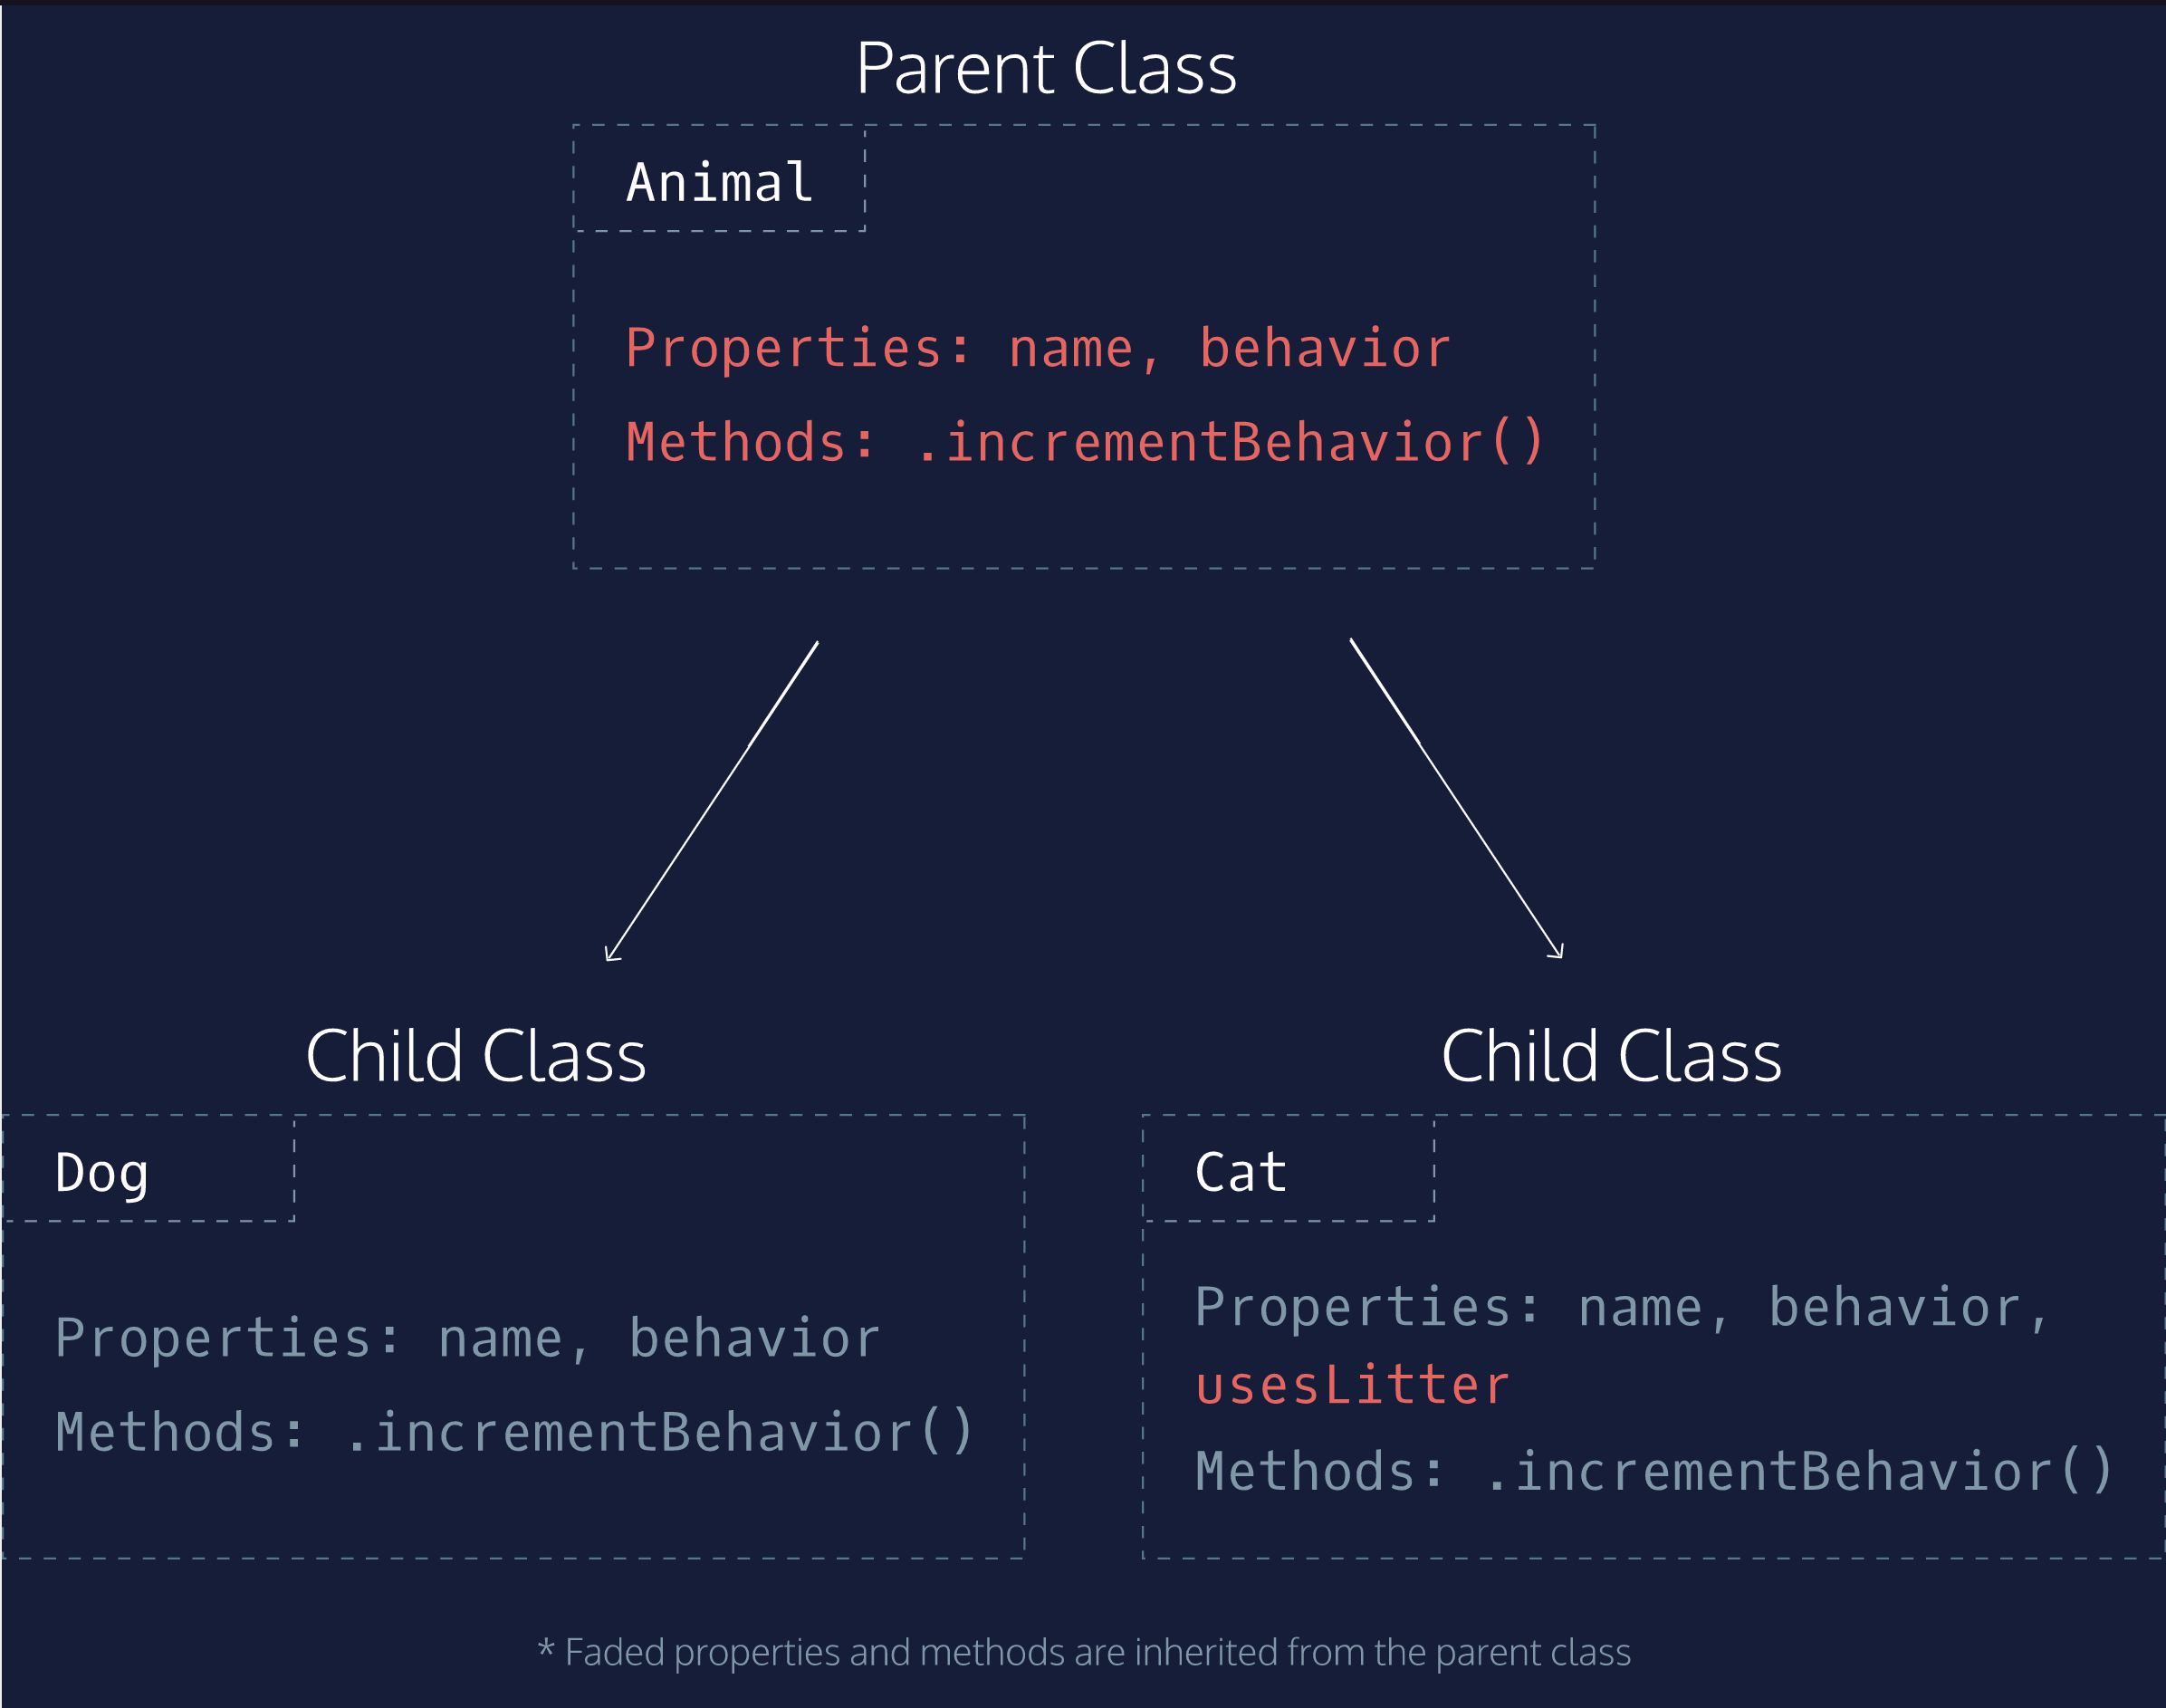
\includegraphics[scale = 0.242]{12_1}
\centering
\end{figure}
Now that we have these shared properties and methods in the parent \colorbox{lightgray}{Animal} class, we can extend them to the subclass, \colorbox{lightgray}{Cat}.
\begin{lstlisting}
class Cat extends Animal {
  constructor(name, usesLitter) {
    super(name);
    this._usesLitter = usesLitter;
  }
}
\end{lstlisting}
In the example above, we create a new class named \colorbox{lightgray}{Cat} that extends the \colorbox{lightgray}{Animal} class. Let us pay special attention to the new keywords: \colorbox{lightgray}{extends} and \colorbox{lightgray}{super}.
\begin{itemize}[leftmargin = *]
\item The \colorbox{lightgray}{extends} keyword makes the methods of the animal class available inside the cat class.
\item The constructor, called when you create a new \colorbox{lightgray}{Cat} object, accepts two arguments, \colorbox{lightgray}{name} and \colorbox{lightgray}{usesLitter}.
\item The \colorbox{lightgray}{super} keyword calls the constructor of the parent class. In this case, \colorbox{lightgray}{super(name)} passes the name argument of the \colorbox{lightgray}{Cat} class to the constructor of the \colorbox{lightgray}{Animal} class. When the \colorbox{lightgray}{Animal} constructor runs, it sets \colorbox{lightgray}{this.\_name = name;} for new \colorbox{lightgray}{Cat} instances.
\item \colorbox{lightgray}{\_usesLitter} is a new property that is unique to the \colorbox{lightgray}{Cat} class, so we set it in the \colorbox{lightgray}{Cat} constructor.
\end{itemize}
Notice, we call \colorbox{lightgray}{super} on the first line of our \colorbox{lightgray}{constructor()}, then set the \colorbox{lightgray}{usesLitter} property on the second line. In a \colorbox{lightgray}{constructor()}, you must always call the \colorbox{lightgray}{super} method before you can use the \colorbox{lightgray}{this} keyword — if you do not, JavaScript will throw a reference error. To avoid reference errors, it is best practice to call \colorbox{lightgray}{super} on the first line of subclass constructors. \\
\newline
Below, we create a new \colorbox{lightgray}{Cat} instance and call its name with the same syntax as we did with the \colorbox{lightgray}{Dog} class:
\begin{lstlisting}
const bryceCat = new Cat("Bryce", false); 
console.log(bryceCat._name); // output: Bryce
\end{lstlisting}
In the example above, we create a new instance the \colorbox{lightgray}{Cat} class, named \colorbox{lightgray}{bryceCat}. We pass it \colorbox{lightgray}{`Bryce'} and \colorbox{lightgray}{false} for our \colorbox{lightgray}{name} and \colorbox{lightgray}{usesLitter} arguments. When we call \colorbox{lightgray}{console.log(bryceCat.\_name)} our program prints, \colorbox{lightgray}{Bryce}. \\
\newline
In the example above, we abandoned best practices by calling our \colorbox{lightgray}{\_name} property directly. In the next exercise, we will address this by calling an inherited getter method for our \colorbox{lightgray}{name} property. \\
\newline
Now that we know how to create an object that inherits properties from a parent class let us turn our attention to methods. When we call extends in a class declaration, all of the parent methods are available to the child class. \\
\newline
Here, we extend our \colorbox{lightgray}{Animal} class to a \colorbox{lightgray}{Cat} subclass.
\newpage
\begin{lstlisting}
class Animal {
  constructor(name) {
    this._name = name;
    this._behavior = 0;
  }

  get name() {
    return this._name;
  }

  get behavior() {
    return this._behavior;
  }

  incrementBehavior() {
    this._behavior++;
  }
} 


class Cat extends Animal {
  constructor(name, usesLitter) {
    super(name);
    this._usesLitter = usesLitter;
  }
}

const bryceCat = new Cat("Bryce", false);
\end{lstlisting}
In the example above, our \colorbox{lightgray}{Cat} class extends \colorbox{lightgray}{Animal}. As a result, the \colorbox{lightgray}{Cat} class has access to the \colorbox{lightgray}{Animal} getters and the \colorbox{lightgray}{.incrementBehavior()} method. \\
\newline
Also in the code above, we create a \colorbox{lightgray}{Cat} instance named \colorbox{lightgray}{bryceCat}. Because \colorbox{lightgray}{bryceCat} has access to the \colorbox{lightgray}{name} getter, the code below logs \colorbox{lightgray}{`Bryce'} to the console. 
\begin{lstlisting}
console.log(bryceCat.name);
\end{lstlisting}
Since the \colorbox{lightgray}{extends} keyword brings all of the parent’s getters and methods into the child class, \colorbox{lightgray}{bryceCat.name} accesses the \colorbox{lightgray}{name} getter and returns the value saved to the \colorbox{lightgray}{name} property. \\
\newline
Now consider a more involved example.
\begin{lstlisting}
bryceCat.incrementBehavior(); // Call .incrementBehavior() on Cat instance 
console.log(bryceCat.behavior); // Log value saved to behavior
\end{lstlisting}
\colorbox{lightgray}{1} is logged to the console. Let us investigate why. 
\begin{itemize}[leftmargin = *]
\item The \colorbox{lightgray}{Cat} class inherits the \colorbox{lightgray}{\_behavior} property, behavior getter, and the \colorbox{lightgray}{.incrementBehavior()} method from the \colorbox{lightgray}{Animal} class.
\item When we created the \colorbox{lightgray}{bryceCat} instance, the  \colorbox{lightgray}{Animal} constructor set the  \colorbox{lightgray}{\_behavior} property to zero.
\item The first line of code calls the inherited  \colorbox{lightgray}{.incrementBehavior()} method, which increases the  \colorbox{lightgray}{bryceCat}  \colorbox{lightgray}{\_behavior} value from zero to one.
\item The second line of code calls the \colorbox{lightgray}{behavior} getter and logs the value saved to  \colorbox{lightgray}{\_behavior} ( \colorbox{lightgray}{1}).
\end{itemize}
In addition to the inherited features, child classes can contain their own properties, getters, setters, and methods. \\
\newline
Below, we will add a \colorbox{lightgray}{usesLitter} getter. The syntax for creating getters, setters, and methods is the same as it is in any other class.
\begin{lstlisting}
class Cat extends Animal {
  constructor(name, usesLitter) {
    super(name);
    this._usesLitter = usesLitter;
  }

  get usesLitter() {
    return this._usesLitter;
  }
}
\end{lstlisting}
In the example above, we create a \colorbox{lightgray}{usesLitter} getter in the \colorbox{lightgray}{Cat} class that returns the value saved to \colorbox{lightgray}{\_usesLitter}.
Compare the \colorbox{lightgray}{Cat} class above to the one we created without inheritance, we decreased the number of lines required to create the \colorbox{lightgray}{Cat} class by about half. It did require an extra class (\colorbox{lightgray}{Animal}). However, the benefits (time saved, readability, efficiency) of inheritance grow as the number and size of your subclasses increase. One benefit is that when you need to change a method or property that multiple classes share, you can change the parent class, instead of each subclass. \\
\newline
Let us see how we would create an additional subclass, called \colorbox{lightgray}{Dog}. 
\begin{lstlisting}
class Dog extends Animal {
  constructor(name) {
    super(name);
  }
}
\end{lstlisting}
This \colorbox{lightgray}{Dog} class has access to the same properties, getters, setters, and methods as the \colorbox{lightgray}{Dog} class we made without inheritance, and is a quarter the size. Now that we have abstracted animal daycare features, it’s easy to see how you can extend Animal to support other classes, like Rabbit, Bird or Snake.

\subsection{Static Methods} 
Sometimes you will want a class to have methods that are not available in individual instances, but that you can call directly from the class.

Take the \colorbox{lightgray}{Date} class, for example — you can both create \colorbox{lightgray}{Date} instances to represent whatever date you want, and call static methods, like \colorbox{lightgray}{Date.now()} which returns the current date, directly from the class. The \colorbox{lightgray}{.now()} method is static, so you can call it directly from the class, but not from an instance of the class.

Let us see how to use the \colorbox{lightgray}{static} keyword to create a static method called \colorbox{lightgray}{generateName} method in our \colorbox{lightgray}{Animal} class:
\begin{lstlisting}
class Animal {
  constructor(name) {
    this._name = name;
    this._behavior = 0;
  }

  static generateName() {
    const names = ["Angel", "Spike", "Buffy", "Willow", "Tara"];
    const randomNumber = Math.floor(Math.random()*5);
    return names[randomNumber];
  }
} 
\end{lstlisting}
In the example above, we create a \colorbox{lightgray}{static} method called \colorbox{lightgray}{.generateName()} that returns a random name when it is called. Because of the \colorbox{lightgray}{static} keyword, we can only access \colorbox{lightgray}{.generateName()} by appending it to the \colorbox{lightgray}{Animal} class. \\
\newline
We call the \colorbox{lightgray}{.generateName()} method with the following syntax:
\begin{lstlisting}
console.log(Animal.generateName()); // returns a name
\end{lstlisting}
You cannot access the \colorbox{lightgray}{.generateName()} method from instances of the \colorbox{lightgray}{Animal} class or instances of its subclasses.
\begin{lstlisting}
const tyson = new Animal("Tyson"); 
tyson.generateName(); // TypeError
\end{lstlisting}
The example above will result in an error, because you cannot call static methods (\colorbox{lightgray}{.generateName()}) on an instance (\colorbox{lightgray}{tyson}).

\subsection{Review: Classes}
\begin{itemize}[leftmargin = *]
\item \textit{Classes} are templates for objects.
\item Javascript calls a \textit{constructor} method when we create a new instance of a class.
\item \textit{Inheritance} is when we create a parent class with properties and methods that we can extend to child classes.
\item We use the \colorbox{lightgray}{extends} keyword to create a subclass.
\item The \colorbox{lightgray}{super} keyword calls the \colorbox{lightgray}{constructor()} of a parent class.
\item Static methods are called on the class, but not on instances of the class.
\end{itemize}

\newpage
\section{Browser Compatibility and Transpilation}
\subsection{Introduction}
Everyone is prompted to update your web browser every few months. A few reasons include addressing security vulnerabilities, adding features, and supporting new HTML, CSS, and JavaScript syntax. The reasons above imply there is a period before a software update is released when there are security vulnerabilities and unsupported language syntax. This chapter focuses on the latter. Specifically, how developers address the gap between the new JavaScript syntax that they use and the JavaScript syntax that web browsers recognize. \\
\newline
This has become a widespread concern for web developers since Ecma International, the organization responsible for standardizing JavaScript, released a new version of it in 2015, called ECMAScript2015, commonly referred to as ES6. Note, the 6 refers to the version of JavaScript and is not related to the year it was released (the previous version was ES5). Upon release, web developers quickly adopted the new ES6 syntax, as it improved readability and efficiency. However, ES6 was not supported by most web browsers, so developers ran into browser compatibility issues. \\
\newline 
This chapter covers two important tools for addressing browser compatibility issues.
\begin{itemize}[leftmargin = *]
\item caniuse.com — A website that provides data on web browser compatibility for HTML, CSS, and JavaScript features. You will learn how to use it to look up ES6 feature support.
\item Babel — A Javascript library that you can use to convert new, unsupported JavaScript (ES6), into an older version (ES5) that is recognized by most modern browsers.
\end{itemize}

\subsection{caniuse.com}
Since Ecma’s release of ECMAScript2015 (ES6), software companies have slowly added support for ES6 features and syntax. While most new browser versions support the majority of the ES6 library, there are still a couple sources of compatibility issues:
\begin{itemize}[leftmargin = *]
\item Some users have not updated to the latest, ES6 supported web browser version.
\item A few ES6 features, like modules, are still not supported by most web browsers.
\end{itemize}
Because companies add support for ES6 features gradually, it is important for you to know how to look up browser support on a feature-by-feature basis. The website \href{https://caniuse.com/}{caniuse.com} is the best resource for finding browser compatibility information.

In caniuse, you can enter an ES6 feature, like \colorbox{lightgray}{let}, and see the percentage of browsers that recognize it. You can also see when each major web browser (Chrome, Safari, Edge, etc.) added support for the keyword.


%The video below shows you how to get started with caniuse.com.
%\includemedia[width=0.6\linewidth,height=0.6\linewidth,activate=pageopen,
%passcontext,
%transparent,
%addresource=caniuse.mov,
%flashvars={source=caniuse.mov}
%]{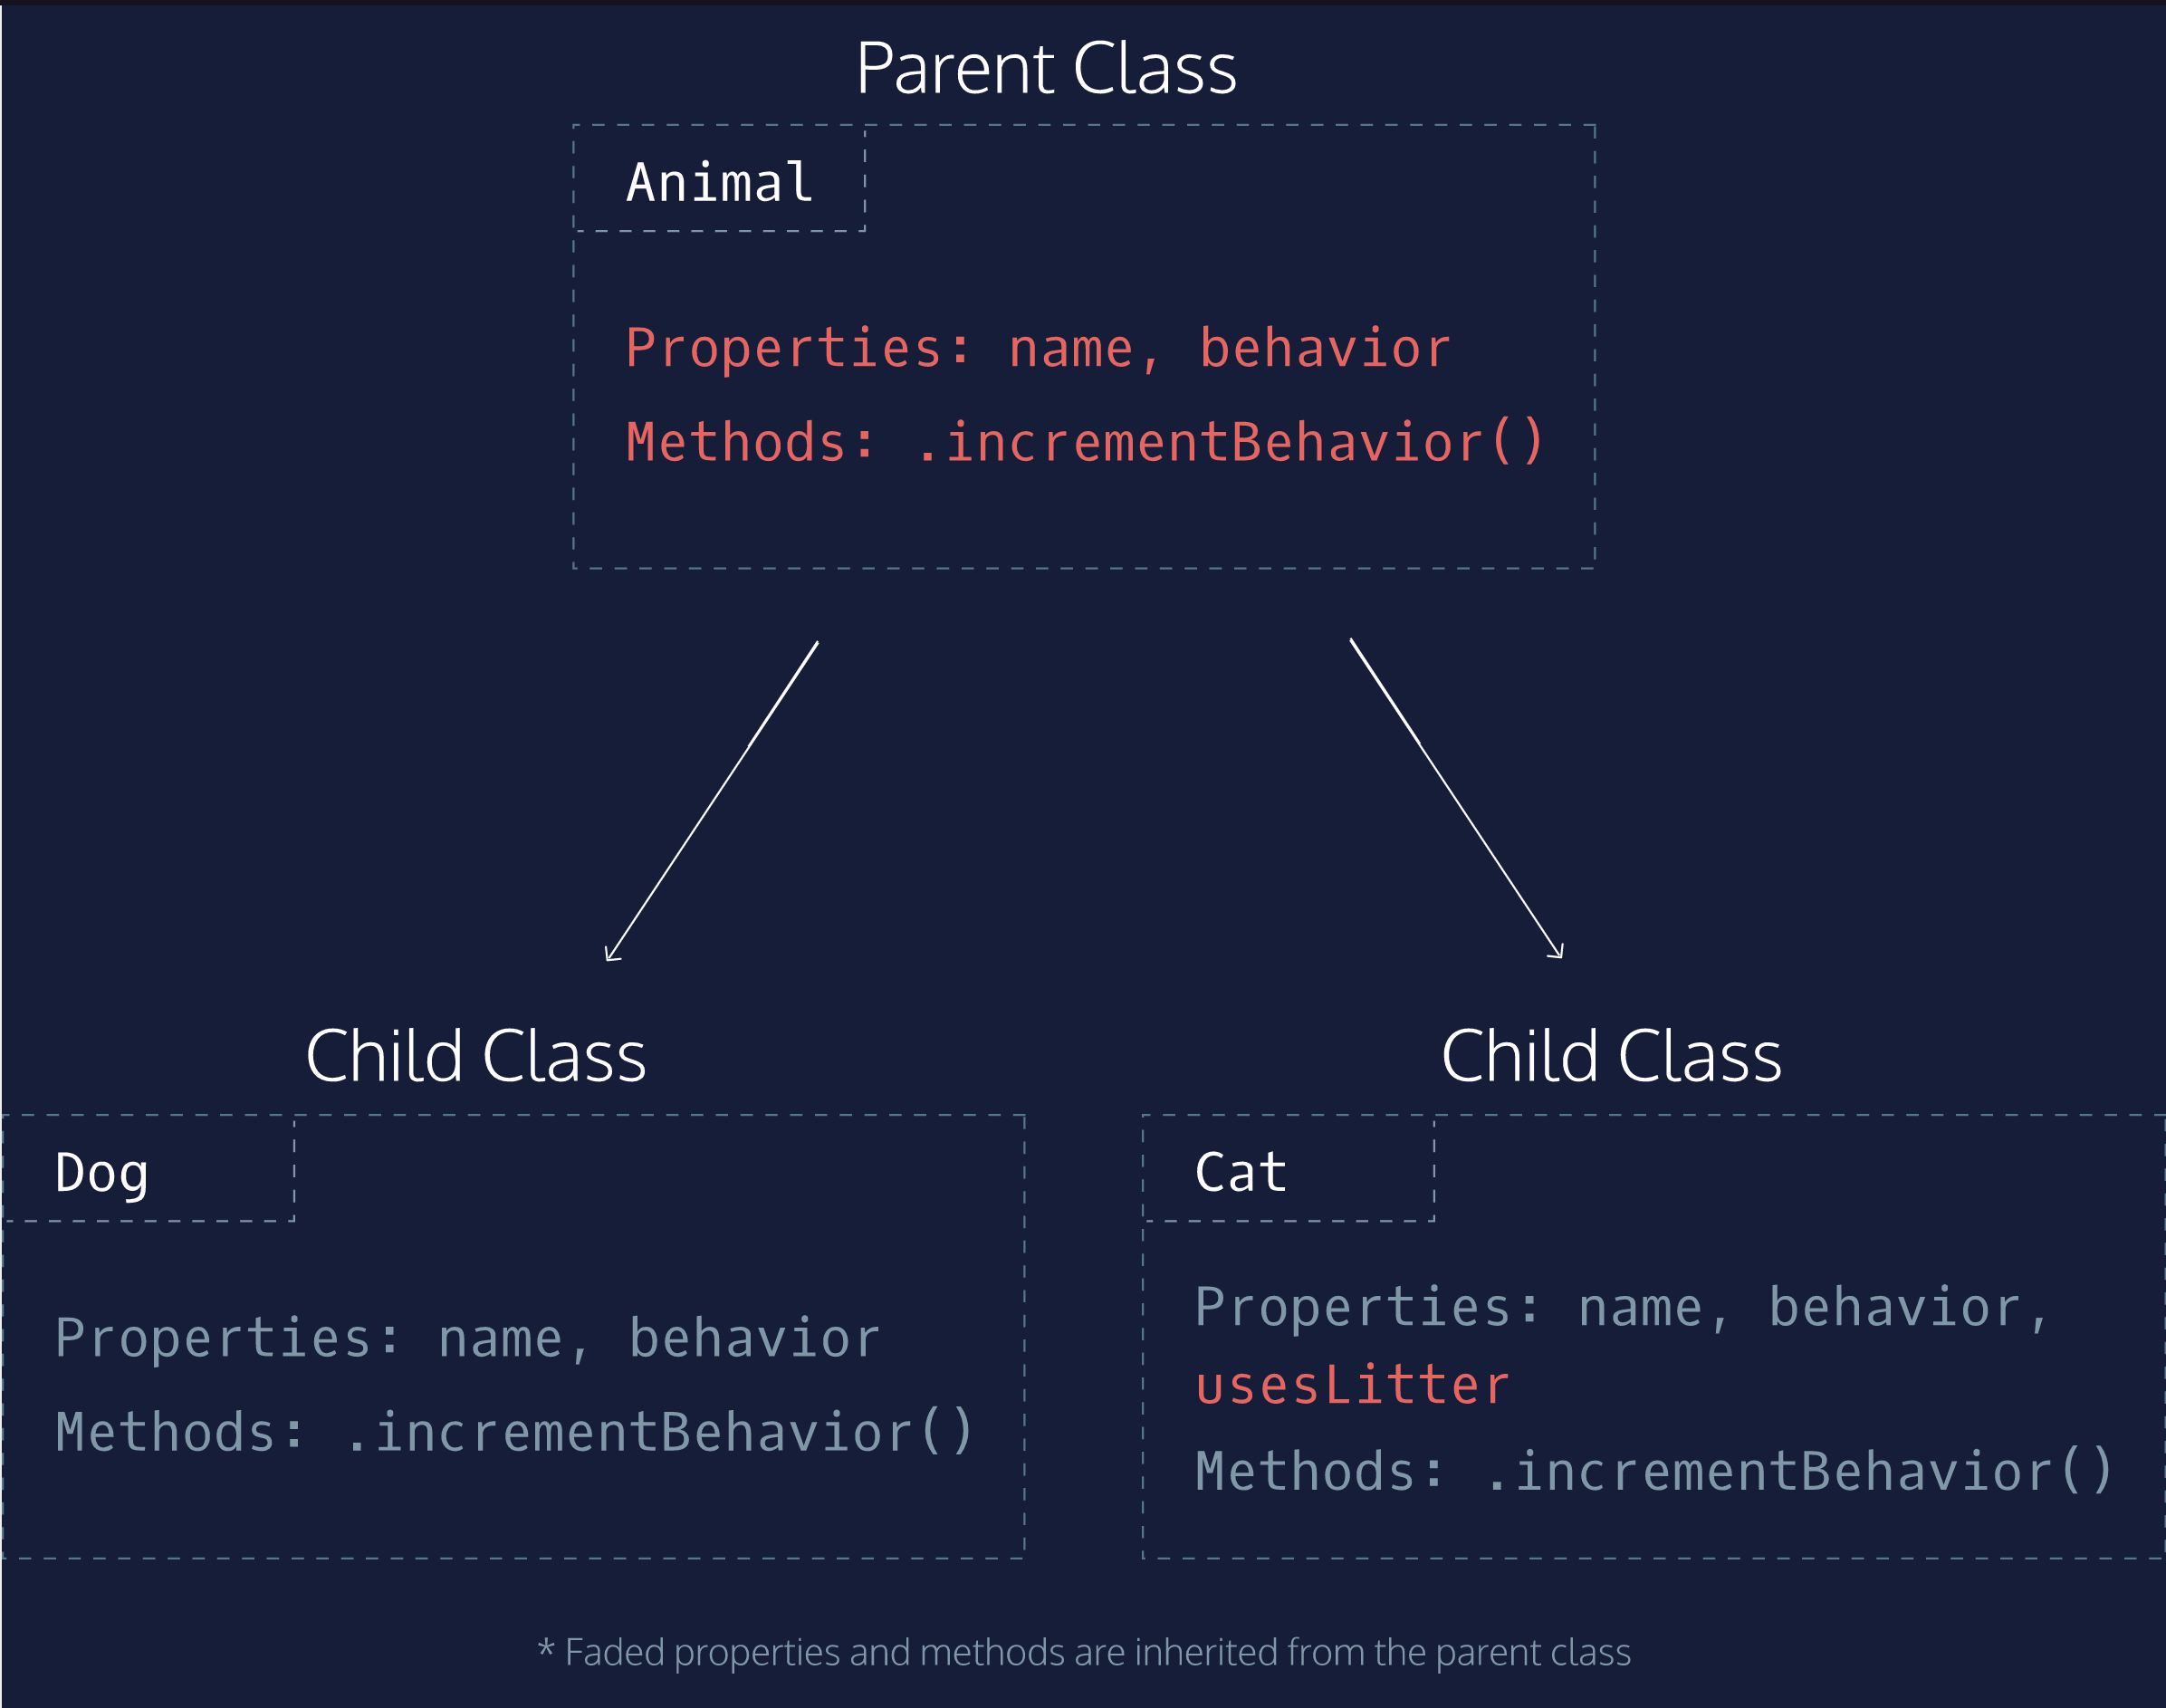
\includegraphics[width=0.6\linewidth]{12_1}}{VPlayer.swf}

\subsection{Why ES6?}
Before we learn how to set up a JavaScript project that converts ES6 to an older version, it is worth understanding a few of the reasons Ecma made such substantial updates. The version of JavaScript that preceded ES6 is called JavaScript ES5. Three reasons for the ES5 to ES6 updates are listed below: 
\begin{itemize}[leftmargin = *]
\item Readability and economy of code — The new syntax is often easier to understand (more readable) and requires fewer characters to create the same functionality (economy of code).
\item Addresses sources of ES5 bugs — Some ES5 syntax led to common bugs. With ES6, Ecma introduced syntax that mitigates some of the most common pitfalls.
\item A similarity to other programming languages — JavaScript ES6 is syntactically more similar to other object-oriented programming languages. This leads to less friction when experienced, non-JavaScript developers want to learn JavaScript.
\end{itemize}
Because ES6 addressed the above issues, Ecma knew that adoption by web developers would occur quickly, while web browser support lagged behind. To limit the impact of ES6 browser compatibility issues, Ecma made the new syntax backwards compatible, which means you can map JavaScript ES6 code to ES5.

\subsection{Transpilation With Babel}
We can manually convert ES6 code to ES5. Although manual conversion only take a few minutes, it is unsustainable as the size of the JavaScript file increases. Because ES6 is predictably backwards compatible, a collection of JavaScript programmers developed a JavaScript library called Babel that \textit{transpiles} ES6 JavaScript to ES5. \textbf{Transpilation is the process of converting one programming language to another.} In the next chapters, we will learn how to use Babel to transpile the new, easy-to-write version of JavaScript (ES6) to the old, browser-compatible version of JavaScript (ES5).
\begin{lstlisting}[basicstyle=\small\ttfamily\color{theWhite}, backgroundcolor = \color{theBlack}, language = Comment]
npm install babel-cli
npm install babel-preset-env
npm run build
\end{lstlisting}

\subsection{npm init}
Next you will learn how to setup a JavaScript project that transpiles code when you run colorbox{lightgray}{npm run build} from the root directory of a JavaScript project. The first step is to place your ES6 JavaScript file in a directory called \textbf{src}. From your root directory, the path to the ES6 file is \textbf{./src/main.js}. The initial JavaScript project file structure is:
\begin{lstlisting}[basicstyle=\small\ttfamily\color{theWhite}, backgroundcolor = \color{theBlack}, language = Comment]
project
|_ src
|___ main.js
\end{lstlisting}
Before we install Babel, we need to setup our project to use the \href{https://docs.npmjs.com/about-npm/index.html}{node package manager (npm)}. Developers use \textit{npm} to access and manage Node packages. Node packages are directories that contain JavaScript code written by other developers. You can use these packages to reduce duplication of work and avoid bugs.

Before we can add Babel to our project directory, we need to run \colorbox{lightgray}{npm init}. The \colorbox{lightgray}{npm init} command creates a \textbf{package.json} file in the root directory. A \textbf{package.json} file contains information about the current JavaScript project. Some of this information includes:
\begin{itemize}[leftmargin = *]
\item Metadata — This includes a project title, description, authors, and more.
\item A list of node packages required for the project — If another developer wants to run your project, npm looks inside \textbf{package.json} and downloads the packages in this list.
\item Key-value pairs for command line scripts — You can use npm to run these shorthand scripts to perform some process. Later, we will add a script that runs Babel and transpiles ES6 to ES5.
\end{itemize}
If you have Node installed on your computer, you can create a \textbf{package.json} file by typing \colorbox{lightgray}{npm init} into the terminal. The terminal prompts you to fill in fields for the project’s metadata (name, description, etc.) You are not required to answer the prompts, though we recommend at minimum, you add your own title and description. If you do not want to fill in a field, you can press enter. npm will leave fill these fields with default values or leave them empty when it creates the \textbf{package.json} file. \\
\newline
After you run \colorbox{lightgray}{npm init} your directory structure will contain the following files and folders:
\begin{lstlisting}[basicstyle=\small\ttfamily\color{theWhite}, backgroundcolor = \color{theBlack}, language = Comment]
project
|_ src
|___ main.js
|_ package.json
\end{lstlisting}

\subsection{Install Node Packages}
We use the npm \colorbox{lightgray}{install} command to install new Node packages locally. The \colorbox{lightgray}{install} command creates a folder called \textbf{node\_modules} and copies the package files to it. The \colorbox{lightgray}{install} command also installs all of the dependencies for the given package. \\
\newline
To install Babel, we need to \colorbox{lightgray}{npm install} two packages, \colorbox{lightgray}{babel-cli} and \colorbox{lightgray}{babel-preset-env}. However, npm installs over one hundred other packages that are dependencies for Babel to run properly. \\
\newline
We install Babel with the following two commands:
\begin{lstlisting}[basicstyle=\small\ttfamily\color{theWhite}, backgroundcolor = \color{theBlack}, language = Comment]
npm install babel-cli -D
npm install babel-preset-env -D
\end{lstlisting}

The \colorbox{lightgray}{babel-cli} package includes command line Babel tools, and the \colorbox{lightgray}{babel-preset-env} package has the code that maps any JavaScript feature, ES6 and above (ES6+), to ES5. \\
\newline
The \colorbox{lightgray}{-D} flag instructs npm to add each package to a property called \colorbox{lightgray}{devDependencies} in \textbf{package.json}. Once the project’s dependencies are listed in \colorbox{lightgray}{devDependencies}, other developers can run your project without installing each package separately. Instead, they can simply run \colorbox{lightgray}{npm install} — it instructs npm to look inside \textbf{package.json} and download all of the packages listed in \colorbox{lightgray}{devDependencies}. \\
\newline
Once you \colorbox{lightgray}{npm install} packages, you can find the Babel packages and all their dependencies in the \textbf{node\_modules} folder. The new directory structure contains the following:
\begin{lstlisting}[basicstyle=\small\ttfamily\color{theWhite}, backgroundcolor = \color{theBlack}, language = Comment]
project
|_ node_modules
|___ .bin
|___ ...
|_ src 
|___ main.js
|_ package.json
\end{lstlisting}
The \colorbox{lightgray}{...} in the file structure above is a placeholder for 100+ packages that npm installed.

\subsection{.babelrc}
Now that we have downloaded the Babel packages, we need to specify the version of the source JavaScript code. We can specify the initial JavaScript version inside of a file named \textbf{.babelrc}. In your root directory, you can run \colorbox{lightgray}{touch .babelrc} to create this file. \\
\newline
Your project directory contains the following folders and files:
\begin{lstlisting}[basicstyle=\small\ttfamily\color{theWhite}, backgroundcolor = \color{theBlack}, language = Comment]
project
|_ node_modules
|___ .bin
|___ ...
|_ src 
|___ main.js
|_ .babelrc
|_ package.json
\end{lstlisting}

Inside \textbf{.babelrc} we need to define the preset for our source JavaScript file. The preset specifies the version of our initial JavaScript file. Usually, we want to transpile JavaScript code from versions ES6 and later (ES6+) to ES5. From this point on, we will refer to our source code as ES6+, because Ecma introduces new syntax with each new version of JavaScript. \\
\newline
To specify that we are transpiling code from an ES6+ source, we have to add the following JavaScript object into \textbf{.babelrc}:
\begin{lstlisting}%[basicstyle=\small\ttfamily\color{theWhite}, backgroundcolor = \color{theBlack}, language = Comment]
{
  "presets": ["env"]
}
\end{lstlisting}
When you run Babel, it looks in \textbf{.babelrc} to determine the version of the initial JavaScript file. In this case, \colorbox{lightgray}{[``env'']} instructs Babel to transpile any code from versions ES6 and later.

\subsection{Babel Source Lib}
There is one last step before we can transpile our code. We need to specify a script in \textbf{package.json} that initiates the ES6+ to ES5 transpilation. 

Inside of the \textbf{package.json} file, there is a property named \colorbox{lightgray}{``scripts''} that holds an object for specifying command line shortcuts. It looks like this:
\begin{lstlisting}%[basicstyle=\small\ttfamily\color{theWhite}, backgroundcolor = \color{theBlack}, language = Comment]
...
"scripts": {
  "test": "echo \"Error: no test specified\" && exit 1"
}, ...
\end{lstlisting}
In the code above, the \colorbox{lightgray}{``scripts''} property contains an object with one property called \colorbox{lightgray}{``test''}. Below the \colorbox{lightgray}{``test''} property, we will add a script that runs Babel like this:
\begin{lstlisting}%[basicstyle=\small\ttfamily\color{theWhite}, backgroundcolor = \color{theBlack}, language = Comment]
...
"scripts": {
  "test": "echo \"Error: no test specified\" && exit 1",
  "build": "babel src -d lib"
}
\end{lstlisting}
In the \colorbox{lightgray}{``scripts''} object above, we add a property called \colorbox{lightgray}{``build''}. The property’s value, \colorbox{lightgray}{``babel src -d lib''}, is a command line method that transpiles ES6+ code to ES5. Let us consider each argument in the method call:
\begin{itemize}[leftmargin = *]
\item \colorbox{lightgray}{babel} — The Babel command call responsible for transpiling code.
\item \colorbox{lightgray}{src} — Instructs Babel to transpile all JavaScript code inside the src directory.
\item \colorbox{lightgray}{-d} — Instructs Babel to write the transpiled code to a directory.
\item \colorbox{lightgray}{lib} — Babel writes the transpiled code to a directory called lib.
\end{itemize}

\subsection{Build}
We are ready to transpile our code. Previously, we wrote the following script in package.json:
\begin{lstlisting}
"build": "babel src -d lib"
\end{lstlisting}
Now, we need to call \colorbox{lightgray}{``build''} from the command line to transpile and write ES5 code to a directory called \colorbox{lightgray}{lib}. From the command line, we type:
\begin{lstlisting}[basicstyle=\small\ttfamily\color{theWhite}, backgroundcolor = \color{theBlack}, language = Comment]
npm run build
\end{lstlisting}
The command above runs the \colorbox{lightgray}{build} script in \textbf{package.json}. Babel writes the ES5 code to a file named \textbf{main.js} (it is always the same name as the original file), inside of a folder called \colorbox{lightgray}{lib}. The resulting directory structure is:
\begin{lstlisting}[basicstyle=\small\ttfamily\color{theWhite}, backgroundcolor = \color{theBlack}, language = Comment]
project
|_ lib
|___ main.js
|_ node_modules
|___ .bin
|___ ...
|_ src
|___ main.js
|_ .babelrc
|_ package.json
\end{lstlisting}
Notice, the directory contains a new folder named \textbf{lib}, with one file, called \textbf{main.js}. \\
\newline
The \colorbox{lightgray}{npm run build} command will transpile all JavaScript files inside of the \textbf{src} folder. This is helpful as you build larger JavaScript projects — regardless of the number of JavaScript files, you only need to run one command (\colorbox{lightgray}{npm run build}) to transpile all of your code.

\subsection{Review}
In this chapter, we learned about browser compatibility and transpilation. Let us review the key concepts:
\begin{itemize}[leftmargin = *]
\item ES5 — The old JavaScript version that is supported by all modern web browsers.
\item ES6 — The new(er) JavaScript version that is \textit{not} supported by all modern web browsers. The syntax is more readable, similar to other programming languages, and addresses the source of common bugs in ES5.
\item caniuse.com — a website you can use to look up HTML, CSS, and JavaScript browser compatibility information.
\item Babel — A JavaScript package that transpiles JavaScript ES6+ code to ES5.
\item \colorbox{lightgray}{npm init} — A terminal command that creates a \textbf{package.json} file.
\item \textbf{package.json} — A file that contains information about a JavaScript project.
\item \colorbox{lightgray}{npm install} — A command that installs Node packages.
\item \colorbox{lightgray}{babel-cli} — A Node package that contains command line tools for Babel.
\item \colorbox{lightgray}{babel-preset-env} — A Node package that contains ES6+ to ES5 syntax mapping information.
\item \textbf{.babelrc} — A file that specifies the version of the JavaScript source code.
\item \colorbox{lightgray}{``build''} script — A \textbf{package.json} script that you use to tranpsile ES6+ code to ES5.
\item \colorbox{lightgray}{npm run build} — A command that runs the \colorbox{lightgray}{build} script and transpiles ES6+ code to ES5.
\end{itemize}
For future reference, here is a list of the steps needed to set up a project for transpilation:
\begin{enumerate}[leftmargin = *]
\item Initialize your project using \colorbox{lightgray}{npm init} and create a directory called \textbf{src}
\item Install babel dependencies by running
\begin{lstlisting}[basicstyle=\small\ttfamily\color{theWhite}, backgroundcolor = \color{theBlack}, language = Comment]
npm install babel-cli -D
npm install babel-preset-env -D
\end{lstlisting}
\item Create a \textbf{.babelrc} file inside your project and add the following code inside it:
\begin{lstlisting}%[basicstyle=\small\ttfamily\color{theWhite}, backgroundcolor = \color{theBlack}, language = Comment]
{
  "presets": ["env"]
}
\end{lstlisting}
\item Add the following script to your \colorbox{lightgray}{scripts} object in \textbf{package.json}:
\begin{lstlisting}
"build": "babel src -d lib"
\end{lstlisting}
\item Run \colorbox{lightgray}{npm run build} whenever you want to transpile your code from your \textbf{src} to \textbf{lib} directories.
\end{enumerate}

\newpage
\section{Intermediate JavaScript Modules}
\subsection{Hello Modules}
JavaScript \textit{modules} are reusable pieces of code that can be exported from one program and imported for use in another program. Modules are particularly useful for a number of reasons. By separating code with similar logic into files called modules, we can:
\begin{itemize}[leftmargin = *]
\item find, fix, and debug code more easily;
\item reuse and recycle defined logic in different parts of our application;
\item keep information private and protected from other modules;
\item and, importantly, prevent pollution of the global namespace and potential naming collisions, by cautiously selecting variables and behavior we load into a program.
\end{itemize}
In this chapter, we will cover two ways to implement modules in JavaScript: \href{https://nodejs.org/en/about/}{Node.js’s} \colorbox{lightgray}{module.exports} and \colorbox{lightgray}{require()} syntax, as well as the ES6 \colorbox{lightgray}{import}/\colorbox{lightgray}{export} syntax.

\subsection{module.exports}
We can get started with modules by defining a module in one file and making the module available for use in another file with Node.js \colorbox{lightgray}{module.exports} syntax. Every JavaScript file run in Node has a local \colorbox{lightgray}{module} object with an \colorbox{lightgray}{exports} property used to define what should be exported from the file. \\
\newline
Below is an example of how to define a module and how to export it using the statement \colorbox{lightgray}{module.exports}. In \textbf{menu.js} we write:
\begin{lstlisting}
let Menu = {};
Menu.specialty = "Roasted Beet Burger with Mint Sauce";

module.exports = Menu; 
\end{lstlisting}
Let us consider what this code means.
\begin{enumerate}[leftmargin = *]
\item let \colorbox{lightgray}{Menu = \{\};} creates the object that represents the module \colorbox{lightgray}{Menu}. The statement contains an uppercase variable named \colorbox{lightgray}{Menu} which is set equal to an empty object.
\item \colorbox{lightgray}{Menu.specialty} is defined as a property of the \colorbox{lightgray}{Menu} module. We add data to the \colorbox{lightgray}{Menu} object by setting properties on that object and giving the properties a value.
\item \colorbox{lightgray}{``Roasted Beet Burger with Mint Sauce'';} is the value stored in the \colorbox{lightgray}{Menu.specialty} property.
\item \colorbox{lightgray}{module.exports = Menu;} exports the \colorbox{lightgray}{Menu} object as a module. \colorbox{lightgray}{module} is a variable that represents the module, and \colorbox{lightgray}{exports} exposes the module as an object.
\end{enumerate}
The pattern we use to export modules is thus:
\begin{enumerate}[leftmargin = *]
\item Create an object to represent the module.
\item Add properties or methods to the module object.
\item Export the module with module.exports.
\end{enumerate}

\subsection{require()}
To make use of the exported module and the behavior we define within it, we import the module into another file. In Node.js, use the \colorbox{lightgray}{require()} function to import modules. \\
\newline
For instance, say we want the module to control the menu’s data and behavior, and we want a separate file to handle placing an order. We would create a separate file \textbf{order.js} and import the \colorbox{lightgray}{Menu} module from \textbf{menu.js} to \textbf{order.js} using \colorbox{lightgray}{require()}. \colorbox{lightgray}{require()} takes a file path argument pointing to the original module file. \\
\newline
In \textbf{order.js} we would write:
\begin{lstlisting}
const Menu = require("./menu.js");

function placeOrder() {
  console.log("My order is: " + Menu.specialty);
}

placeOrder();
\end{lstlisting}
We now have the entire behavior of \colorbox{lightgray}{Menu} available in \textbf{order.js}. Here, we notice:
\begin{enumerate}[leftmargin = *]
\item In \textbf{order.js} we import the module by creating a \colorbox{lightgray}{const} variable called \colorbox{lightgray}{Menu} and setting it equal to the value of the \colorbox{lightgray}{require()} function. We can set the name of this variable to anything we like, such as \colorbox{lightgray}{menuItems}. 
\item \colorbox{lightgray}{require()} is a JavaScript function that loads a module. Its argument is the file path of the module: \colorbox{lightgray}{./menu.js}. With \colorbox{lightgray}{require()}, the \colorbox{lightgray}{.js} extension is optional and will be assumed if it is not included.
\item The \colorbox{lightgray}{placeOrder()} function then uses the \colorbox{lightgray}{Menu} module. By calling \colorbox{lightgray}{Menu.specialty}, we access the property \colorbox{lightgray}{specialty} defined in the \colorbox{lightgray}{Menu} module.
\end{enumerate}
Taking a closer look, the pattern to import a module is:
\begin{enumerate}[leftmargin = *]
\item Import the module with \colorbox{lightgray}{require()} and assign it to a local variable.
\item Use the module and its properties within a program.
\end{enumerate}

\subsection{module.exports II}
We can also wrap any collection of data and functions in an object, and export the object using \colorbox{lightgray}{module.exports}. In \textbf{menu.js}, we could write:
\begin{lstlisting}
module.exports = {
  specialty: "Roasted Beet Burger with Mint Sauce",
  getSpecialty: function() {
    return this.specialty;
  } 
}; 
\end{lstlisting}
In the above code, notice:
\begin{enumerate}[leftmargin = *]
\item \colorbox{lightgray}{module.exports} exposes the current module as an object.
\item \colorbox{lightgray}{specialty} and \colorbox{lightgray}{getSpecialty} are properties on the object.
\end{enumerate}
Then in \textbf{order.js}, we write:
\begin{lstlisting}
const Menu = require("./menu.js");

console.log(Menu.getSpecialty());
\end{lstlisting}
Here we can still access the behavior in the \colorbox{lightgray}{Menu} module.

\subsection{export default}
Node.js supports \colorbox{lightgray}{require()}/\colorbox{lightgray}{module.exports}, but as of ES6, JavaScript supports a new more readable and flexible syntax for exporting modules. These are usually broken down into one of two techniques, \textit{default export} and \textit{named exports}. \\
\newline
We will begin with the first syntax, default export. The default export syntax works similarly to the \colorbox{lightgray}{module.exports} syntax, allowing us to export one module per file. \\
\newline
Let us look at an example in \textbf{menu.js}.
\begin{lstlisting}
let Menu = {};

export default Menu;
\end{lstlisting}
\begin{enumerate}[leftmargin = *]
\item \colorbox{lightgray}{export default} uses the JavaScript \colorbox{lightgray}{export} statement to export JavaScript objects, functions, and primitive data types.
\item \colorbox{lightgray}{Menu} refers to the name of the \colorbox{lightgray}{Menu} object, the object that we are setting the properties on within our modules.
\end{enumerate}
When using ES6 syntax, we use \colorbox{lightgray}{export default} in place of \colorbox{lightgray}{module.exports}. Node.js does not support \colorbox{lightgray}{export default} by default, so \colorbox{lightgray}{module.exports} is usually used for Node.js development and ES6 syntax is used for front-end development. As with most ES6 features, it is common to transpile code since ES6 is \href{https://caniuse.com/#search=sd}{not supported by all browsers}.

\subsection{import}
ES6 module syntax also introduces the \colorbox{lightgray}{import} keyword for importing objects. In our \textbf{order.js} example, we import an object like this:
\begin{lstlisting}
import Menu from "./menu";
\end{lstlisting}
\begin{enumerate}[leftmargin = *]
\item The \colorbox{lightgray}{import} keyword begins the statement.
\item The keyword \colorbox{lightgray}{Menu} here specifies the name of the variable to store the default export in.
\item \colorbox{lightgray}{from} specifies where to load the module from.
\item \colorbox{lightgray}{`./menu'} is the name of the module to load. When dealing with local files, it specifically refers to the name of the file without the extension of the file.
\end{enumerate}
We can then continue using the \colorbox{lightgray}{Menu} module in the \textbf{order.js} file.

\subsection{Named Exports}
ES6 introduced a second common approach to export modules. In addition to \colorbox{lightgray}{export default}, \textit{named exports} allow us to export data through the use of variables. \\
\newline
Let us see how this works. In \textbf{menu.js} we would be sure to give each piece of data a distinct variable name:
\begin{lstlisting}
let specialty = "";
function isVegetarian() {
}; 
function isLowSodium() {
}; 

export { specialty, isVegetarian };
\end{lstlisting}
\begin{enumerate}[leftmargin = *]
\item Notice that, when we use named exports, we are not setting the properties on an object. Each export is stored in its own variable.
\item \colorbox{lightgray}{specialty} is a string object, while \colorbox{lightgray}{isVegetarian} and \colorbox{lightgray}{isLowSodium} are objects in the form of functions. Recall that in JavaScript, every function is in fact a function object.
\item \colorbox{lightgray}{export \{ specialty, isVegetarian \};} exports objects by their variable names. Notice the keyword \colorbox{lightgray}{export} is the prefix.
\item \colorbox{lightgray}{specialty} and \colorbox{lightgray}{isVegetarian} are exported, while \colorbox{lightgray}{isLowSodium} is not exported, since it is not specified in the export syntax.
\end{enumerate}

\subsection{Named Imports}
To import objects stored in a variable, we use the \colorbox{lightgray}{import} keyword and include the variables in a set of \colorbox{lightgray}{\{\}}. In the \textbf{order.js} file, for example, we would write:
\begin{lstlisting}
import { specialty, isVegetarian } from "./menu";

console.log(specialty);
\end{lstlisting}
\begin{enumerate}[leftmargin = *]
\item Here \colorbox{lightgray}{specialty} and \colorbox{lightgray}{isVegetarian} are imported.
\item If we did not want to import either of these variables, we could omit them from the \colorbox{lightgray}{import} statement.
\item We can then use these objects as in within our code. For example, we would use \colorbox{lightgray}{specialty} instead of \colorbox{lightgray}{Menu.specialty}.
\end{enumerate}

\subsection{Export Named Exports}
Named exports are also distinct in that they can be exported as soon as they are declared, by placing the keyword \colorbox{lightgray}{export} in front of variable declarations. \\
\newline
In \textbf{menu.js}
\begin{lstlisting}
export let specialty = "";
export function isVegetarian() {
}; 
function isLowSodium() {
}; 
\end{lstlisting}
\begin{enumerate}[leftmargin = *]
\item The \colorbox{lightgray}{export} keyword allows us to export objects upon declaration, as shown in \colorbox{lightgray}{export let specialty} and \colorbox{lightgray}{export function isVegetarian() \{\}}.
\item We no longer need an \colorbox{lightgray}{export} statement at the bottom of our file, since this behavior is handled above.
\end{enumerate}

\subsection{Import Named Imports}
To import variables that are declared, we simply use the original syntax that describes the variable name. In other words, exporting upon declaration does not have an impact on how we import the variables.
\begin{lstlisting}
import { specialty, isVegetarian } from "menu";
\end{lstlisting}

\subsection{Export as}
Named exports also conveniently offer a way to change the name of variables when we export or import them. We can do this with the \colorbox{lightgray}{as} keyword. Let us see how this works. In our \textbf{menu.js} example:
\begin{lstlisting}
let specialty = "";
let isVegetarian = function() {
}; 
let isLowSodium = function() {
}; 

export { specialty as chefsSpecial, isVegetarian as isVeg, isLowSodium };
\end{lstlisting}
In the above example, take a look at the \colorbox{lightgray}{export} statement at the bottom of the of the file.
\begin{enumerate}[leftmargin = *]
\item The \colorbox{lightgray}{as} keyword allows us to give a variable name an alias as demonstrated in \colorbox{lightgray}{specialty as chefsSpecial} and \colorbox{lightgray}{isVegetarian as isVeg}.
\item Since we did not give \colorbox{lightgray}{isLowSodium} an alias, it will maintain its original name.
\end{enumerate}

\subsection{Import as}
To import named export aliases with the \colorbox{lightgray}{as} keyword, we add the aliased variable in our import statement.
\begin{lstlisting}
import { chefsSpecial, isVeg } from "./menu";
\end{lstlisting}
In \textbf{orders.js}
\begin{enumerate}[leftmargin = *]
\item We import \colorbox{lightgray}{chefsSpecial} and \colorbox{lightgray}{isVeg} from the \colorbox{lightgray}{Menu} object.
\item Here, note that we have an option to alias an object that was not previously aliased when exported. For example, the \colorbox{lightgray}{isLowSodium} object that we exported could be aliased with the as keyword when imported: 
\end{enumerate}
\begin{lstlisting}
import {isLowSodium as saltFree} from "Menu";
\end{lstlisting}
Another way of using aliases is to import the entire module as an alias:
\begin{lstlisting}
import * as Carte from "./menu";

Carte.chefsSpecial;
Carte.isVeg();
Carte.isLowSodium(); 
\end{lstlisting}
\begin{enumerate}[leftmargin = *]
\item This allows us to import an entire module from \textbf{menu.js} as an alias \colorbox{lightgray}{Carte}.
\item In this example, whatever name we exported would be available to us as properties of that module. For example, if we exported the aliases \colorbox{lightgray}{chefsSpecial} and \colorbox{lightgray}{isVeg}, these would be available to us. If we did not give an alias to \colorbox{lightgray}{isLowSodium}, we would call it as defined on the \colorbox{lightgray}{Carte} module.
\end{enumerate}

\subsection{Combining Export Statements}
We can also use named exports and default exports together. In \textbf{menu.js}:
\begin{lstlisting}
let specialty = "";
function isVegetarian() {
}; 
function isLowSodium() {
}; 
function isGlutenFree() {
};

export { specialty as chefsSpecial, isVegetarian as isVeg };
export default isGlutenFree;
\end{lstlisting}
Here we use the keyword \colorbox{lightgray}{export} to export the named exports at the bottom of the file. Meanwhile, we export the \colorbox{lightgray}{isGlutenFree} variable using the \colorbox{lightgray}{export default} syntax. This would also work if we exported most of the variables as declared and exported others with the \colorbox{lightgray}{export default} syntax.
\begin{lstlisting}
export let Menu = {};

export let specialty = "";
export let isVegetarian = function() {
}; 
export let isLowSodium = function() {
}; 
let isGlutenFree = function() {
};

export default isGlutenFree;
\end{lstlisting}
Here we use the \colorbox{lightgray}{export} keyword to export the variables upon declaration, and again export the \colorbox{lightgray}{isGlutenFree} variable using the \colorbox{lightgray}{export default syntax}. \\
\newline
While it is better to avoid combining two methods of exporting, it is useful on occasion. For example, if you suspect developers may only be interested in importing a specific function and will not need to import the entire default export.

\subsection{Combining Import Statements}
We can import the collection of objects and functions with the same data. We can use an \colorbox{lightgray}{import} keyword to import both types of variables as such:
\begin{lstlisting}
import { specialty, isVegetarian, isLowSodium } from "./menu";

import GlutenFree from "./menu";
\end{lstlisting}

\subsection{Review}
Let us review what we learned about JavaScript modules: \\
\newline
\textit{Modules} in Node.js are reusable pieces of code that can be exported from one program and imported for use in another program.
\begin{itemize}[leftmargin = *]
\item \colorbox{lightgray}{module.exports} exports the module for use in another program.
\item \colorbox{lightgray}{require()} imports the module for use in the current program.
\end{itemize}
ES6 introduced a more flexible, easier syntax to export modules:
\begin{itemize}[leftmargin = *]
\item default exports use \colorbox{lightgray}{export default} to export JavaScript objects, functions, and primitive data types.
\item named exports use the \colorbox{lightgray}{export} keyword to export data in variables.
\item named exports can be aliased with the \colorbox{lightgray}{as} keyword.
\item \colorbox{lightgray}{import} is a keyword that imports any object, function, or data type.
\end{itemize}



\newpage
\section{Promises}
\newpage
\section{Async-Await}
\newpage
\section{Requests}






\end{document}
